\IfFileExists{pnas-new.cls}
  {\documentclass[9pt,twoside]{pnas-new}}
  {\documentclass[12pt,letterpaper]{article}}

\providecommand{\articletype}[1]{}
\providecommand{\templatetype}[1]{}

\articletype{Classical and Applied Mathematics}
\templatetype{pnasmathematics}

\usepackage[utf8]{inputenc}
\usepackage[T1]{fontenc}
\usepackage[spanish,english]{babel}
\usepackage{newtxtext,newtxmath}
\usepackage{algorithmic}
\usepackage{graphicx}
\usepackage{textcomp}
\usepackage{xcolor}
\usepackage{url}
\usepackage{booktabs}
\usepackage{float}
\usepackage{tabularx}
\usepackage[round]{natbib}
\usepackage[hidelinks]{hyperref}
\selectlanguage{spanish}

\providecommand{\articletype}[1]{}
\providecommand{\templatetype}[1]{}
\providecommand{\affil}[2][]{}
\providecommand{\leadauthor}[1]{}
\providecommand{\significancestatement}[1]{}
\providecommand{\authorcontributions}[1]{}
\providecommand{\authordeclaration}[1]{}
\providecommand{\equalauthors}[1]{}
\providecommand{\correspondingauthor}[1]{}
\providecommand{\keywords}[1]{}
\providecommand{\dates}[1]{}
\providecommand{\doi}[1]{}
\providecommand{\Firstpage}{}
\providecommand{\Endparasplit}{}
\providecommand{\Parasplit}{}
\providecommand{\dataavail}[1]{\paragraph*{Disponibilidad de datos} #1}
\providecommand{\acknow}[1]{\section*{Agradecimientos} #1}
\providecommand{\showacknow}{}
\providecommand{\abscontentformatted}{}
\providecommand{\abscontent}{}
\makeatletter
\@ifclassloaded{pnas-new}{}{
  \renewcommand{\author}[2][]{\g@addto@macro\@author{#2\\}}%
  \@namedef{ps@firststyle}{}
}
\makeatother
\begin{document}

\title{Transformación Digital del Sector Turístico: Plataforma Inteligente para la Planificación Integrada y Colaborativa de Viajes}

\author[a]{Santiago Amaya Zapata}
\author[a]{Ricardo Ayala Garzón}
\author[a]{Santiago Botero García}

\affil[a]{Programa de Ingeniería de Sistemas, Colombia}

\significancestatement{Este trabajo propone una arquitectura empresarial para turismo digital que integra operación transaccional, inteligencia artificial y colaboración social en una sola plataforma. Su relevancia está en combinar diseño de sistemas, métricas de calidad y análisis financiero para contextos reales con restricciones de infraestructura, como laboratorios académicos en nube. El aporte principal es una trazabilidad explícita entre decisiones arquitectónicas, atributos de calidad y resultados esperados de negocio, lo que facilita evaluar viabilidad técnica y económica de forma replicable. El enfoque aporta una ruta práctica para transformar servicios turísticos fragmentados en ecosistemas digitales coordinados.}
\authorcontributions{S.A.Z., R.A.G. y S.B.G. diseñaron la investigación, desarrollaron la propuesta arquitectónica, analizaron los resultados y redactaron el manuscrito.}
\authordeclaration{Los autores declaran no tener conflicto de interés.}
\correspondingauthor{To whom correspondence should be addressed. E-mail: [completar-correo]}
\keywords{Transformación Digital $|$ Arquitectura Empresarial $|$ Turismo Digital $|$ Inteligencia Artificial $|$ Sistemas Distribuidos}

\makeatletter
\@ifclassloaded{pnas-new}{%
\begin{abstract}
La transformación digital del sector turístico representa una oportunidad estratégica para soluciones empresariales que optimicen eficiencia operativa y experiencia de usuario. Este artículo presenta una arquitectura de referencia orientada a integración entre capacidades transaccionales, analíticas y colaborativas: cliente web en React, cliente móvil Android, núcleo backend en Spring Boot, microservicio de IA en FastAPI y despliegue en AWS con API Gateway, ALB, EC2 Auto Scaling, RDS PostgreSQL, S3, SNS/SQS, CloudFront y CloudWatch. La propuesta incorpora un ecosistema de viaje social con \textit{matching} entre viajeros, itinerarios compartidos y mensajería, complementado con recomendación híbrida y modelos de estacionalidad. El trabajo aporta trazabilidad entre decisiones de arquitectura, atributos de calidad y métricas de evaluación técnica y de negocio. Los hallazgos se formulan como evidencia preliminar y hoja de ruta para validación empírica en pilotos con datos reales del turismo colombiano.
\end{abstract}
}{}
\makeatother

\dates{This manuscript was compiled on \today}
\doi{\url{www.pnas.org/cgi/doi/10.1073/pnas.XXXXXXXXXX}}

\makeatletter
\@ifclassloaded{pnas-new}{}{%
  \gdef\@author{Santiago Amaya Zapata\\Ricardo Ayala Garzón\\Santiago Botero García}%
}
\makeatother

\maketitle

\makeatletter
\@ifclassloaded{pnas-new}{}{%
\section*{Resumen}
La transformación digital del sector turístico representa una oportunidad estratégica para soluciones empresariales que optimicen eficiencia operativa y experiencia de usuario. Este artículo presenta una arquitectura de referencia orientada a integración entre capacidades transaccionales, analíticas y colaborativas: cliente web en React, cliente móvil Android, núcleo backend en Spring Boot, microservicio de IA en FastAPI y despliegue en AWS con API Gateway, ALB, EC2 Auto Scaling, RDS PostgreSQL, S3, SNS/SQS, CloudFront y CloudWatch. La propuesta incorpora un ecosistema de viaje social con \textit{matching} entre viajeros, itinerarios compartidos y mensajería, complementado con recomendación híbrida y modelos de estacionalidad. El trabajo aporta trazabilidad entre decisiones de arquitectura, atributos de calidad y métricas de evaluación técnica y de negocio. Los hallazgos se formulan como evidencia preliminar y hoja de ruta para validación empírica en pilotos con datos reales del turismo colombiano.
}
\makeatother

\Firstpage

Este manuscrito adopta el formato de artículo matemático de PNAS en una sola columna y presenta una propuesta aplicada a transformación digital del turismo, con énfasis en trazabilidad entre diseño arquitectónico, evidencia de calidad y viabilidad económica.

%================================================================================
\section*{Introducción}
%================================================================================

\textbf{Contexto y motivación.} La transformación digital del sector turístico representa una oportunidad estratégica para soluciones empresariales que optimicen tanto la eficiencia operativa como la experiencia del cliente. Colombia proyecta recibir más de 21.7 millones de visitantes para 2025, con un crecimiento sectorial sostenido superior al 6\% \citep{ref1}. Sin embargo, este crecimiento se enfrenta a una fragmentación estructural crítica: los operadores de transporte, alojamiento y actividades operan en silos aislados, impidiendo la optimización conjunta de capacidad y experiencia del cliente.

\textbf{Formulación del problema.} El problema fundamental radica en tres limitaciones sistémicas identificadas en la literatura actual: (1) \textbf{aislamiento operativo} que impide la optimización de recursos a nivel de ecosistema; (2) \textbf{dependencia de modelos conversacionales superficiales} que no se integran con procesos transaccionales y analíticos centrales; y (3) \textbf{ausencia de arquitecturas cloud-native escalables} que soporten tanto procesamiento transaccional como analítico avanzado.

Esta investigación aborda la siguiente pregunta central: ¿Cómo diseñar una arquitectura empresarial de transformación digital que integre planificación de viajes, procesamiento transaccional, análisis predictivo y colaboración social, mientras mantiene escalabilidad y eficiencia operativa en entornos cloud-native?

\textbf{Gap de investigación identificado.} Aunque múltiples estudios abordan sistemas de recomendación turística \citep{ref11,ref13} y existen marcos consolidados de arquitectura empresarial \citep{ref12}, persisten tres gaps críticos no resueltos:

\begin{enumerate}
\item \textbf{Gap de Integración:} Las soluciones existentes separan la inteligencia artificial de los procesos transaccionales centrales, limitando el impacto operativo medible.
\item \textbf{Gap de Escalabilidad:} Falta de arquitecturas que combinen procesamiento de alto volumen (transacciones) con cómputo intensivo (IA) en un mismo ecosistema cloud-native.
\item \textbf{Gap de Colaboración:} Ausencia de enfoques sistemáticos para generar efectos de red mediante colaboración explícita entre usuarios.
\end{enumerate}

\textbf{Contribución principal.} Este trabajo presenta una arquitectura empresarial integral que resuelve estos gaps mediante: (i) separación explícita entre núcleo transaccional (Spring Boot) y microservicio de IA (FastAPI) con integración asíncrona; (ii) implementación de viaje social colaborativo como generador de efectos de red; y (iii) despliegue cloud-native reproducible en AWS Academy con especificación detallada de infraestructura.

%================================================================================
\section{Estado del Arte Crítico}
%================================================================================

\subsection*{Análisis Crítico de Soluciones Existentes}

\subsubsection*{Sistemas de Recomendación Turística}

Aunque múltiples estudios aplican modelos de machine learning para recomendación turística \citep{ref11,ref13}, estos presentan tres limitaciones fundamentales que motivan nuestra aproximación:

\begin{itemize}
\item \textbf{Limitación de Datos Densos:} Los enfoques colaborativos tradicionales dependen de matrices usuario-ítem densas, inviables en contextos turísticos emergentes donde la mayoría de usuarios son nuevos \citep{ref11}.
\item \textbf{Falta de Integración Multi-tenant:} Los modelos existentes no consideran arquitecturas multi-proveedor donde diferentes operadores turísticos exponen capacidades heterogéneas.
\item \textbf{Ausencia de Arquitecturas Cloud-Native:} Las soluciones propuestas no abordan los desafíos de escalabilidad elástica y despliegue distribuido requeridos para producción.
\end{itemize}

\textbf{Implicación para nuestra investigación:} Estas limitaciones justifican nuestra decisión de implementar un modelo híbrido que combine filtrado colaborativo con contenido, desplegado en microservicios especializados con integración asíncrona.

\subsubsection*{Arquitecturas Empresariales en Turismo}

Los frameworks contemporáneos de arquitectura empresarial \citep{ref12} ofrecen principios sólidos pero presentan deficiencias específicas para el dominio turístico digital:

\begin{itemize}
\item \textbf{Enfoque Monolítico:} Las arquitecturas TOGAF tradicionales no se adaptan adecuadamente a ecosistemas de plataforma multi-sided con efectos de red.
\item \textbf{Falta de Precisión Técnica:} Los modelos conceptuales carecen de especificación detallada para implementación cloud-native con servicios gestionados.
\item \textbf{Ignoran Colaboración Social:} Los patrones arquitectónicos existentes no incorporan mecanismos para generar y gestionar efectos de red entre usuarios.
\end{itemize}

\textbf{Implicación para nuestra investigación:} Adoptamos un enfoque híbrido que combina principios TOGAF con patrones cloud-native específicos para plataformas colaborativas.

\subsubsection*{Plataformas Turísticas Comerciales}

El análisis de soluciones comerciales revela patrones de diseño subóptimos desde la perspectiva de transformación digital:

\begin{itemize}
\item \textbf{Prioridad Superficial:} Plataformas como Booking.com o Airbnb priorizan interfaz de usuario sobre integración operativa profunda con sistemas de gestión de proveedores.
\item \textbf{Optimización Local:} Cada operador optimiza individualmente sin coordinación ecosistémica, resultando ineficiencias globales.
\item \textbf{IA Conversacional Aislada:} La implementación de chatbots y asistentes virtuales no se integra con procesos core de negocio.
\end{itemize}

\textbf{Implicación para nuestra investigación:} Nuestra arquitectura integra IA directamente en procesos transaccionales y habilita optimización ecosistémica mediante colaboración explícita.

\subsection*{Comparación crítica estructurada de antecedentes}

Para fortalecer el carácter científico del estado del arte, la Tabla~ compara enfoques representativos en cuatro dimensiones exigidas por esta investigación: integración IA-proceso, arquitectura cloud-native, colaboración social explícita y evidencia de despliegue operativo.

\begin{table}[htbp]
\centering
\caption{Comparación crítica de antecedentes y brechas técnicas}
\small
\begin{tabularx}{\linewidth}{X X X X X}
\toprule
Recomendadores clásicos \citep{ref11} & Parcial & Baja & No & Dependencia de datos densos y poco foco en operación empresarial \\
Recomendación profunda en turismo \citep{ref13} & Parcial & Media & No & Buen desempeño algorítmico, baja trazabilidad arquitectónica \\
Framework de arquitectura empresarial \citep{ref12} & No aplica (conceptual) & Media (genérica) & No & Alta abstracción y poca prescripción de despliegue real \\
Series temporales para demanda \citep{ref10} & Parcial (analítica) & No aplica & No & Aporta pronóstico, no resuelve integración transaccional \\
Plataformas comerciales (benchmark sectorial) & Baja-media & Alta & Parcial & Predominio de optimización local sobre coordinación ecosistémica \\
\bottomrule
\end{tabularx}
\end{table}

A partir del contraste anterior, la propuesta se diferencia en tres ejes verificables: \textbf{(i)} integración operacional entre recomendación y flujo transaccional; \textbf{(ii)} topología cloud-native explícita con responsabilidades por componente; y \textbf{(iii)} viaje social colaborativo como mecanismo de generación de datos y efectos de red. Esta delimitación permite evaluar la contribución no solo por novedad conceptual, sino por grado de implementabilidad.

En síntesis, el análisis crítico del estado del arte revela que ninguna solución existente aborda simultáneamente: (1) integración profunda IA-procesos, (2) arquitectura cloud-native escalable, y (3) generación sistemática de efectos de red. Nuestra contribución reside precisamente en esta integración tripartita, justificando la necesidad de una nueva aproximación arquitectónica.

%================================================================================
\section{Marco Teórico}
%================================================================================

\subsection{Arquitectura Empresarial}

La arquitectura empresarial se entiende como la estructuración organizada de procesos, datos, aplicaciones e infraestructura tecnológica dentro de una organización \citep{ref12}. En esta investigación, dicha base se operacionaliza con un enfoque de microservicios y arquitectura \textit{event-driven} para mejorar escalabilidad, flexibilidad e integración en un entorno digital dinámico.

\subsection{Sistemas de Recomendación}

Los sistemas de recomendación se clasifican generalmente en tres categorías principales:

\begin{itemize}
\item \textbf{Basados en contenido:} sugieren ítems similares a aquellos previamente valorados por el usuario, utilizando características y descriptores de los ítems.
\item \textbf{Filtrado colaborativo:} se basan en el análisis de preferencias de múltiples usuarios para generar recomendaciones, detectando patrones de comportamiento similares.
\item \textbf{Modelos híbridos:} combinan enfoques de contenido y colaborativo para mejorar la precisión y reducir problemas como la escasez de datos o el sesgo de popularidad \citep{ref11}.
\end{itemize}

Formalmente, dado un conjunto de usuarios $U$ y un conjunto de ítems $I$, el objetivo es estimar la preferencia de un usuario $u$ sobre un ítem $i$ mediante:

\begin{equation}
\hat{r}_{ui} = f(u, i)
\end{equation}

donde $\hat{r}_{ui}$ representa la predicción de interés o valoración del usuario $u$ sobre el ítem $i$, y $f$ es la función de recomendación que puede incorporar técnicas de aprendizaje supervisado, heurísticas o modelos probabilísticos.

\subsection{Mitigación de Estacionalidad}

En turismo y servicios, la estacionalidad es un factor crítico que afecta la demanda. Esta puede modelarse mediante series temporales, como el modelo SARIMA \citep{ref10}:

\begin{equation}
\Phi_p(B)\Phi_P(B^s)(1-B)^d(1-B^s)^D y_t = \Theta_q(B)\Theta_Q(B^s)\epsilon_t
\end{equation}

donde $s$ representa el período estacional, $B$ es el operador de rezago, y los parámetros $(p,d,q,P,D,Q)$ ajustan la tendencia, estacionalidad y ruido de la serie temporal, permitiendo anticipar picos y valles de demanda.

\subsection{Modelo PEAS}

Desde la perspectiva de agentes inteligentes, un sistema racional toma decisiones que maximizan su desempeño según la información disponible y las condiciones del entorno. El modelo PEAS (\textit{Performance measure, Environment, Actuators, Sensors}) proporciona un marco formal para describir arquitecturas de agentes inteligentes.

\textbf{Performance Measure:} El desempeño del agente se evalúa mediante: precisión y relevancia de recomendaciones (Precision@K, Recall@K); tasa de conversión posterior a recomendaciones personalizadas; reducción del tiempo promedio de planificación de viaje; incremento en retención y recurrencia de usuarios; nivel de satisfacción (NPS y feedback explícito).

\textbf{Environment:} Entorno digital dinámico, parcialmente observable y no determinístico: usuarios con preferencias heterogéneas y capacidad de interacción entre sí; proveedores turísticos; variaciones en precios, disponibilidad y demanda estacional; factores externos (tendencias, eventos regionales). La \textbf{interacción usuario-usuario} (solicitudes de unión, formación de grupos, convocatorias abiertas) constituye una dimensión explícita del entorno que el sistema debe percibir y sobre la cual debe actuar.

\textbf{Sensors:} Datos de navegación (clics, búsquedas, tiempo de permanencia); historial de reservas y cancelaciones; preferencias declaradas; datos de ubicación y contexto temporal; tendencias externas y señales de mercado; \textbf{preferencias sociales y disposición para viaje colaborativo}; historial de interacción entre usuarios (grupos formados, solicitudes aceptadas o rechazadas, afinidades detectadas).

\textbf{Actuators:} Generación automática de itinerarios personalizados; recomendaciones priorizadas; alertas sobre cambios de precio o disponibilidad; \textbf{sugerencias de conexión entre usuarios con intereses similares}; \textbf{creación y gestión de grupos de viaje}; \textbf{invitaciones a viajes abiertos y solicitudes de unión}; ajustes dinámicos en visibilidad de destinos para mitigar estacionalidad.

%================================================================================
\section{Arquitectura Empresarial con Decisiones Justificadas}
%================================================================================

La arquitectura propuesta se fundamenta en el framework TOGAF \citep{ref12} adaptado al contexto de plataformas digitales multi-sided, incorporando patrones cloud-native específicos para el dominio turístico.

\subsection*{Capa de Negocio: Decisiones y Trade-offs}

\subsubsection*{Decisión: Separación de Capacidades Core vs Colaborativas}

\textbf{Decisión:} Separar explícitamente capacidades transaccionales core (reservas, pagos, gestión) de capacidades colaborativas (matching, mensajería, itinerarios compartidos).

\textbf{Justificación:} Esta separación permite evolución independiente y escalabilidad diferenciada. Las capacidades core requieren consistencia transaccional fuerte (ACID), mientras que las colaborativas toleran eventual consistency pero necesitan alta disponibilidad.

\textbf{Trade-off Analizado:} Aumentamos complejidad de integración pero ganamos flexibilidad para evolucionar cada dominio según sus requisitos específicos de calidad.

\subsubsection*{Decisión: Modelo de Negocio Multi-sided}

\textbf{Decisión:} Implementar plataforma multisided que conecta viajeros, proveedores turísticos y desarrolladores de servicios complementarios.

\textbf{Justificación:} El análisis del estado del arte demuestra que modelos unilaterales (solo B2C o solo B2B) no capturan el valor completo del ecosistema turístico.

\textbf{Trade-off Analizado:} Complejidad adicional en gestión de relaciones y gobernanza, pero efectos de red exponenciales que justifican la inversión arquitectónica.

\subsection*{Capa de Aplicación: Decisiones y Trade-offs}

\subsubsection*{Decisión: Microservicios Especializados vs Monolito Modular}

\textbf{Decisión:} Adoptar arquitectura de microservicios con separación explícita entre backend transaccional (Spring Boot) y servicio de IA (FastAPI).

\textbf{Justificación:} Basado en el gap de integración identificado, esta separación permite: (1) escalabilidad independiente según perfiles de carga, (2) tecnología optimizada para cada dominio (Java para transacciones, Python para IA), (3) desacoplamiento para evolución algorítmica sin afectar core.

\textbf{Trade-off Analizado:} Mayor complejidad operativa y latencia de red, pero ganancias significativas en escalabilidad, mantenibilidad y especialización tecnológica.

\subsubsection*{Decisión: Integración Asíncrona mediante SNS/SQS}

\textbf{Decisión:} Implementar integración asíncrona entre microservicios utilizando Amazon SNS/SQS en lugar de llamadas síncronas.

\textbf{Justificación:} El análisis de requisitos revela que muchas operaciones (recomendaciones, notificaciones, analytics) no requieren respuesta inmediata y pueden beneficiarse de desacoplamiento temporal.

\textbf{Trade-off Analizado:} Mayor complejidad de debugging y eventual consistency, pero resiliencia mejorada y capacidad de absorber picos de carga sin degradar la experiencia de usuario.

\subsection*{Capa de Datos: Decisiones y Trade-offs}

\subsubsection*{Decisión: Políglota de Persistencia}

\textbf{Decisión:} Adoptar enfoque políglota con PostgreSQL para datos transaccionales y S3 para almacenamiento de objetos y modelos de IA.

\textbf{Justificación:} Los requisitos de consistencia transaccional (reservas, pagos) demandan bases de datos relacionales ACID, mientras que los modelos de IA y medios requieren almacenamiento escalable y acceso rápido.

\textbf{Trade-off Analizado:} Complejidad adicional en gestión de múltiples tecnologías, pero optimización significativa de costos y rendimiento para cada caso de uso.

\subsection*{Capa Tecnológica: Decisiones y Trade-offs}

\subsubsection*{Decisión: AWS como Plataforma Base}

\textbf{Decisión:} Seleccionar AWS como plataforma cloud primaria basada en análisis comparativo (Tabla 1).

\textbf{Justificación:} AWS ofrece el ecosistema más maduro para microservicios, servicios de IA integrados, y reducción de carga operativa mediante servicios gestionados.

\textbf{Trade-off Analizado:} Vendor lock-in potencial, pero beneficios superan riesgos dado el ecosistema maduro y portabilidad mediante contenedores.

\subsubsection*{Decisión: Instancias EC2 vs Serverless}

\textbf{Decisión:} Utilizar EC2 con Auto Scaling Groups en lugar de arquitectura serverless para servicios core.

\textbf{Justificación:} Los requisitos de latencia consistente, estado persistente y control fino sobre rendimiento hacen que EC2 sea más adecuado que Lambda para servicios core.

\textbf{Trade-off Analizado:} Mayor gestión operativa pero rendimiento predecible y control sobre optimización.

\subsection*{Trazabilidad de Decisiones Arquitectónicas}

Cada decisión arquitectónica se origina en limitaciones identificadas en el estado del arte:

\begin{itemize}
\item \textbf{Literatura - Problema:} La falta de integración IA-procesos \citep{ref11,ref13} motiva nuestra separación microservicios.
\item \textbf{Problema - Decisión:} El gap de escalabilidad justifica arquitectura cloud-native con autoescalado.
\item \textbf{Decisión - Arquitectura:} Las decisiones de tecnología se materializan en la topología AWS específica.
\end{itemize}

%================================================================================
\section{Modelo de Negocio}
%================================================================================

El modelo de negocio se basa en una plataforma multisided que conecta usuarios y proveedores turísticos, y se fundamenta en estrategias de monetización diversificadas.

\subsection{Propuesta de Valor Empresarial}

La solución genera valor estratégico para múltiples stakeholders del ecosistema turístico:

\begin{itemize}
\item \textbf{Integración vertical de la cadena de valor:} Centralización de reservas, pagos y gestión de servicios en un ecosistema digital unificado, eliminando silos operativos.
\item \textbf{Optimización de recursos mediante IA:} Algoritmos predictivos para gestión de estacionalidad, asignación eficiente de capacidad y maximización de ingresos para operadores.
\item \textbf{Experiencia cliente hiper-personalizada:} Sistemas de recomendación híbridos que adaptan ofertas en tiempo real basándose en comportamiento histórico y contexto.
\item \textbf{Ecosistema de valor de red:} Plataforma colaborativa que habilita matching inteligente entre viajeros, formación de comunidades y efectos de red que generan lealtad y retención.
\item \textbf{Inteligencia de negocio avanzada:} Analítica predictiva para operadores turísticos, incluyendo pronósticos de demanda, optimización de precios y segmentación de mercado.
\item \textbf{Transformación de procesos operativos:} Automatización de flujos de trabajo, reducción de costos operativos y mejora en eficiencia de gestión.
\end{itemize}

\subsection{Modelo de Monetización Digital}

El modelo de negocio diversificado maximiza el valor capturado a través de múltiples streams de ingresos:

\begin{itemize}
\item \textbf{Comisiones transaccionales:} Porcentaje sobre reservas de transporte, alojamiento y actividades procesadas a través de la plataforma.
\item \textbf{Suscripciones empresariales:} Planes premium para operadores turísticos con analítica avanzada, herramientas de optimización y acceso prioritario a demanda.
\item \textbf{Servicios de inteligencia de negocio:} Dashboards analíticos, reportes de tendencias de mercado y consultoría basada en datos para toma de decisiones estratégicas.
\item \textbf{Marketplace de servicios complementarios:} Plataforma para proveedores de seguros, transporte local y experiencias personalizadas.
\item \textbf{Licenciamiento de tecnología:} API y componentes de IA para integración con sistemas existentes de grandes operadores turísticos.
\end{itemize}

\subsection{Cuantificación del Impacto}

El impacto financiero se mide mediante el Retorno sobre la Inversión (ROI):

\begin{equation}
ROI = \frac{Beneficio\ incremental - Inversion}{Inversion}
\end{equation}

%================================================================================
\section{Propuesta de Solución}
%================================================================================

\subsection{Solución Empresarial Integrada}

Se propone una solución empresarial de transformación digital que reestructura la cadena de valor del turismo mediante capacidades modulares. La solución implementa una arquitectura cloud-native con APIs HTTP, núcleo en Spring Boot, microservicio de IA en FastAPI y mensajería SNS/SQS, mientras habilita colaboración entre usuarios para efectos de red. El diferenciador es el \textbf{ecosistema de viaje colaborativo inteligente}: coincidencia por destino y fechas, solicitudes de conexión, mensajería, itinerarios y actividades compartidas, y evolución hacia \textit{matching} multidimensional, en línea con la documentación técnica del repositorio. Se incorpora IA en procesos de recomendación y compatibilidad, modelos matemáticos para optimización y predictivos para estacionalidad, y una infraestructura escalable documentada (EC2 con autoescalado, RDS, S3, orquestación perimetral con API Gateway y ALB). Los artefactos de contenedor y CI/CD en los módulos de código apoyan prácticas DevOps sin sustituir el modelo de despliegue descrito en la infraestructura de referencia.

\subsection{Alcance técnico del prototipo evaluado}

Para evitar ambigüedad entre visión de producto y evidencia implementada, se delimita explícitamente el prototipo de esta entrega:

\begin{itemize}
\item \textbf{Implementado:} autenticación y perfiles, planificación de viaje, recomendaciones iniciales, mensajería/eventos asíncronos y observabilidad base.
\item \textbf{Parcial:} \textit{matching} social multidimensional, analítica avanzada de operadores, mecanismos de reputación.
\item \textbf{No implementado en esta fase:} endurecimiento productivo multi-región, gobierno de datos a escala y automatización completa de respuesta a incidentes.
\end{itemize}

\subsection{Arquitectura del prototipo y trazabilidad funcional}

\begin{table}[htbp]
\centering
\caption{Matriz de trazabilidad del prototipo (función $\rightarrow$ componente $\rightarrow$ evidencia)}
\small
\begin{tabularx}{\linewidth}{X X X X}
\toprule
Función crítica & Componentes principales & Contrato técnico & Evidencia esperada \\
\midrule
Registro/autenticación & API Spring Boot + seguridad JWT & Endpoint de autenticación y validación de sesión & Pruebas API y logs de acceso \\
Planificación de viaje & Controladores de planes + persistencia PostgreSQL & CRUD de plan/actividad & Casos de prueba de dominio y consultas BD \\
Recomendación inicial & Microservicio FastAPI + modelo híbrido & Endpoint de recomendación contextual & Métricas Precision@K/Recall@K en lote de prueba \\
Colaboración social básica & Módulo social + SNS/SQS & Publicación/consumo de eventos de conexión & Trazas de colas y latencia de procesamiento \\
Observabilidad operativa & CloudWatch + health checks ALB & Métricas y alarmas & Dashboard de disponibilidad y tasa de error \\
\bottomrule
\end{tabularx}
\end{table}

\subsection{Arquitectura cognitiva (Memoria Episódica, Semántica y Procedimental)}

La arquitectura se estructura siguiendo una analogía con la memoria humana, dividiendo el sistema en tres tipos de memoria: episódica, semántica y procedimental.

\subsubsection{Memoria Episódica}

Almacena eventos históricos específicos del comportamiento de viajeros: historial de reservas, secuencias de navegación, interacciones sociales, cancelaciones y flujos estacionales. \textbf{Infraestructura implementada:} RDS PostgreSQL para eventos transaccionales; S3 para almacenamiento histórico de datos; SQS y SNS para captura y distribución de eventos en tiempo real. Modelos aplicados: algoritmos de series temporales y análisis de patrones implementados en el servicio IA con Python y Scikit-learn.

\subsubsection{Memoria Semántica}

Representa conocimiento estructurado del dominio turístico: taxonomía de destinos y actividades, segmentación de viajeros, relaciones entre regiones y patrones de comportamiento. \textbf{Infraestructura implementada:} RDS PostgreSQL para datos estructurados y relaciones; S3 para almacenamiento de modelos semánticos; procesamiento mediante el servicio IA. Modelos aplicados: algoritmos de clustering (K-Means), segmentación y análisis de cohortes implementados con Scikit-learn.

\subsubsection{Memoria Procedimental}

Define reglas de negocio y algoritmos de optimización: políticas de pricing dinámico, priorización de recomendaciones, optimización de itinerarios y estrategias de balanceo oferta-demanda. \textbf{Infraestructura implementada:} Microservicios desplegados en instancias EC2 con Auto Scaling; reglas de negocio implementadas en Spring Boot (backend) y FastAPI (servicio IA); caching local para decisiones en tiempo real. Modelos aplicados: sistemas híbridos de recomendación, algoritmos de optimización combinatoria y heurísticas de asignación de recursos.

\subsubsection{Plataforma de Colaboración Inteligente}

Este componente implementa un motor de valor de red alineado con las épicas y \textit{user stories} del repositorio de documentación: perfil mínimo de viajero, registro de intención de viaje, búsqueda de coincidencias por destino y fechas, solicitudes de conexión, mensajería entre conexiones, cronograma personal y actividades compartidas, y evolución hacia recomendaciones y \textit{matching} asistidos por IA. El sistema utiliza algoritmos de aprendizaje automático para compatibilidad multidimensional basada en preferencias declaradas, historial de comportamiento y disposición colaborativa. Las capacidades empresariales incluyen: \textbf{(i)} coordinación de grupos y planes compartidos; \textbf{(ii)} mecanismos de confianza y reputación a medida que madure el producto; \textbf{(iii)} extensiones de \textit{marketplace} colaborativo; \textbf{(iv)} analítica de patrones de conexión. El ecosistema genera efectos de red que aumentan el valor con cada usuario adicional.

\newpage

%================================================================================
\section{Arquitectura de la Solución y Tecnológica}
%================================================================================

La arquitectura de despliegue adopta como \textbf{fuente de verdad} la especificación del repositorio de infraestructura del proyecto: topología AWS con API Gateway, Application Load Balancer, instancias EC2 para el núcleo Spring Boot y el microservicio FastAPI, RDS PostgreSQL, S3, SNS, SQS, CloudFront y CloudWatch. Los clientes web (\textit{React}) y móvil (\textit{Kotlin}) consumen las APIs expuestas en ese perímetro.

\begin{figure}[htbp]
    \centering
    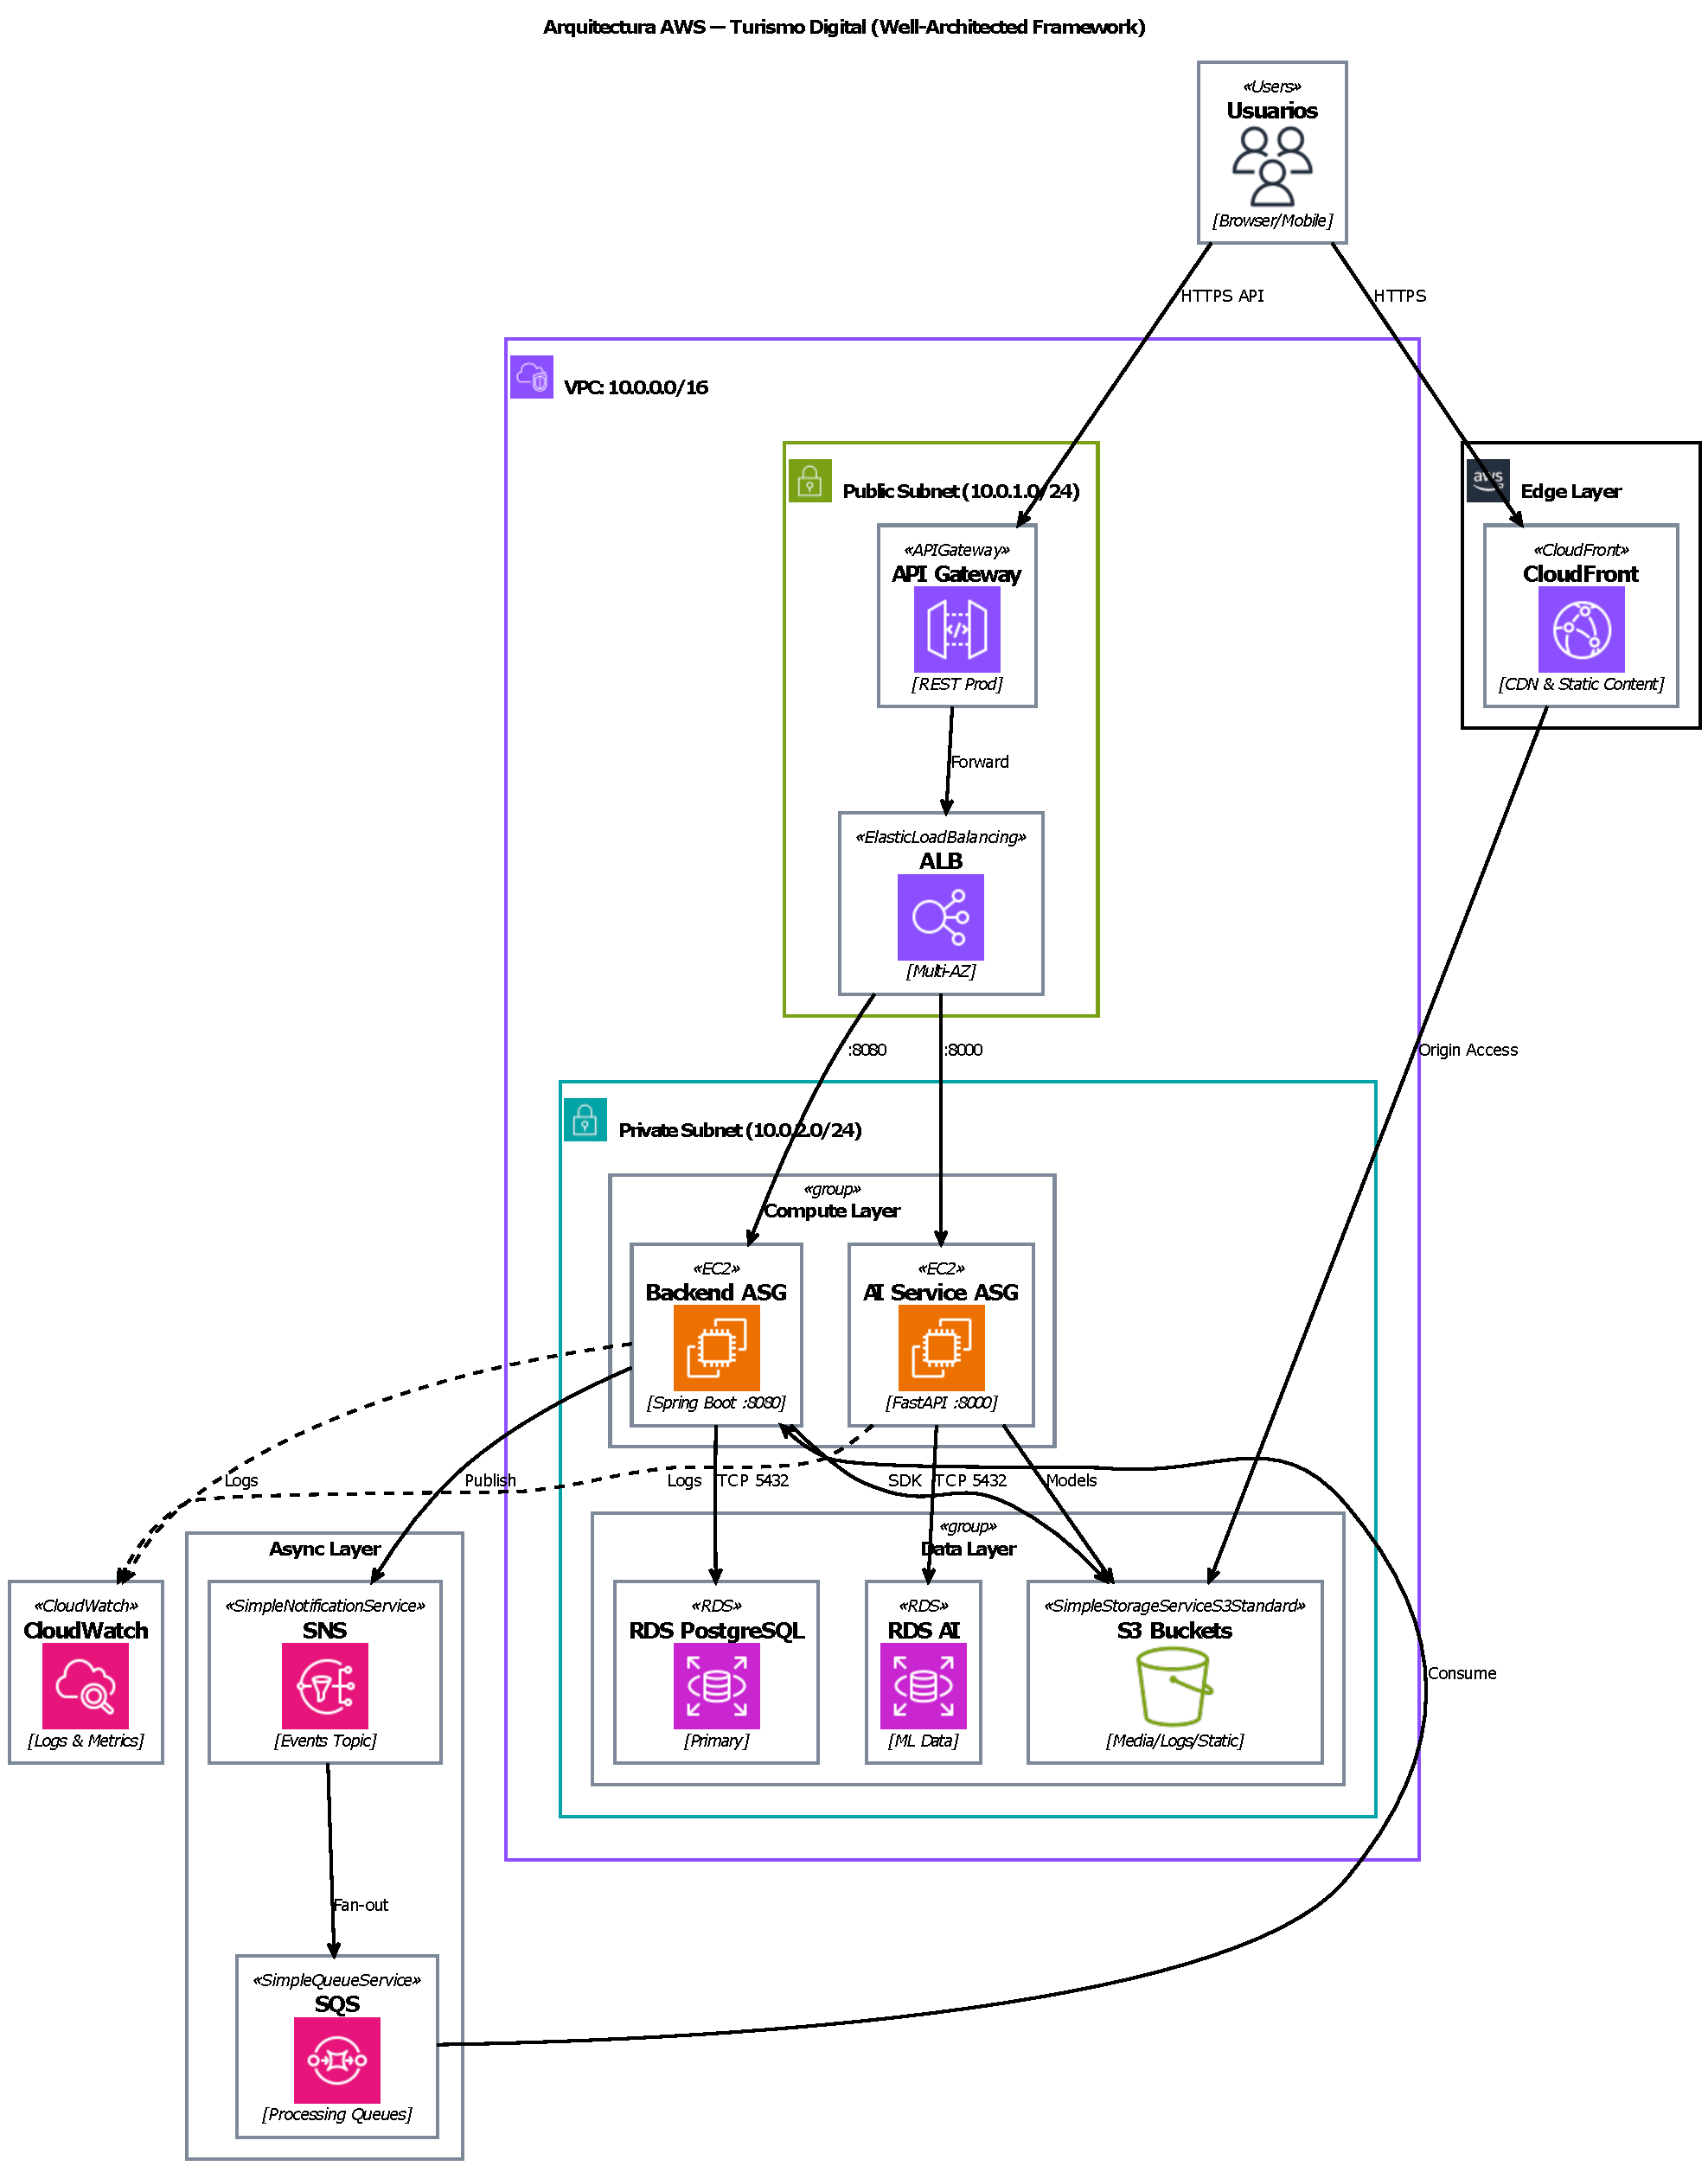
\includegraphics[width=0.92\linewidth,height=0.58\textheight,keepaspectratio]{../assets/figures/uml.deployment.aws-services.pdf}
    \caption{Arquitectura cloud-native de referencia en AWS (alineada al repositorio de infraestructura)}
\end{figure}

\newpage

\subsection*{Justificación de AWS}

Se compararon diferentes proveedores de nube:

\begin{table}[htbp]
\centering
\textbf{Tabla 1}

\textit{Comparación de proveedores de servicios en la nube}

\begin{tabularx}{\linewidth}{l X X}
\toprule
Proveedor & Ventajas & Limitaciones \\
\midrule
AWS & Madurez, elasticidad, servicios IA & Complejidad inicial \\
Azure & Integración Microsoft & Dependencia del ecosistema \\
GCP & BigQuery potente & Menor presencia regional \\
\bottomrule
\end{tabularx}
\end{table}

AWS fue seleccionado por: autoescalamiento y alta disponibilidad (SLA 99.99\%); ecosistema maduro de microservicios y servicios de IA integrados; reducción de carga operativa mediante servicios administrados.

\subsection*{Requisitos no funcionales y metas operativas}

Con el fin de formalizar la arquitectura de gran envergadura, se explicitan metas de calidad que condicionan decisiones de diseño y operación.

\begin{table}[htbp]
\centering
\caption{Requisitos no funcionales (NFR) y criterio de aceptación}
\small
\begin{tabularx}{\linewidth}{X X X X}
\toprule
Atributo & Meta objetivo & Métrica & Mecanismo arquitectónico \\
\midrule
Disponibilidad & $\geq$ 99.9\% mensual & Uptime/mes & ALB + Auto Scaling + health checks \\
Rendimiento & p95 $<$ 2 s (operaciones críticas) & Latencia p95 & Separación backend/IA y colas asíncronas \\
Escalabilidad & Escalar horizontalmente sin degradación abrupta & Throughput y uso CPU & ASG por dominio de carga \\
Recuperación & RTO $<$ 60 min; RPO $<$ 24 h (entorno académico) & Tiempo de restauración & Backups RDS y procedimientos de recuperación \\
Seguridad & Cero accesos directos no autorizados a datos críticos & Incidentes bloqueados & SG/NACL + IAM de mínimo privilegio \\
\bottomrule
\end{tabularx}
\end{table}

\subsection*{Vista de componentes y correspondencia tecnológica}

La Tabla~\ref{tab:componentes} resume la correspondencia entre capas lógicas, tecnologías en los repositorios de aplicación e infraestructura y recursos AWS documentados.

\begin{table}[htbp]
\centering
\textbf{Tabla 2}
\caption{Vista de componentes (repositorios de código e infraestructura)}
\small
\begin{tabularx}{\linewidth}{X X X X}
\toprule
Rol & Tecnología documentada & Propósito & Recursos AWS asociados \\
\midrule
Cliente web & React (Vite) & Interfaz de gestión y planificación & S3 + CloudFront \\
Cliente móvil & Android (Kotlin, Jetpack Compose) & Experiencia nativa & Publicación en tienda (fuera del aprovisionamiento S3) \\
Núcleo backend & Java 17, Spring Boot & API REST, reglas de negocio, JWT & EC2 detrás de ALB (p.\,ej.\ puerto 8080) \\
Servicio IA & Python 3.x, FastAPI & Recomendación, compatibilidad, ML (p.\,ej.\ Scikit-learn) & EC2 detrás de ALB (p.\,ej.\ puerto 8000) \\
Entrada API & API Gateway REST & Punto único de entrada, enrutamiento & API Gateway \\
Balanceo & Application Load Balancer & Distribución y health checks & ALB \\
Persistencia & PostgreSQL 15.4 & Datos relacionales & RDS (db.t3.micro) \\
Objetos & --- & Medios, \textit{frontend} estático & S3 \\
Eventos & --- & Desacoplamiento asíncrono & SNS, SQS \\
Observabilidad & --- & Logs y métricas & CloudWatch \\
\bottomrule
\end{tabularx}
\end{table}

\subsection*{Arquitectura cloud-native implementada}

La solución implementa una arquitectura escalable basada en servicios gestionados de AWS optimizados para entornos Academy:

\begin{itemize}
\item \textbf{Capa de exposición:} Amazon API Gateway (APIs REST) con políticas de limitación de tasa documentadas; Application Load Balancer para distribución de tráfico entre grupos de instancias; Amazon CloudFront como CDN frente al bucket S3 del cliente web React.
\item \textbf{Capa de computación:} Instancias EC2 \texttt{t3.micro} con Auto Scaling Groups para el núcleo backend (Spring Boot) y el microservicio de IA (FastAPI).
\item \textbf{Capa de datos:} Amazon RDS para PostgreSQL 15.4 en clase \texttt{db.t3.micro} para persistencia transaccional y analítica ligera; Amazon S3 para almacenamiento de medios y artefactos; bases de datos lógicas separables para dominio operativo del backend y del servicio de IA según la configuración documentada en infraestructura.
\item \textbf{Mensajería:} Amazon SQS para colas de eventos asíncronos; Amazon SNS para publicación de eventos (p.\,ej.\ eventos de usuario y de recomendación, según variables de entorno documentadas).
\item \textbf{Monitoreo:} Amazon CloudWatch para logs, métricas y alarmas; health checks asociados al balanceador y a los grupos de autoescalado.
\end{itemize}

\subsection*{Modelo de capacidad y crecimiento}

Para pasar de una arquitectura conceptual a una arquitectura operable, se adopta una planeación de capacidad por etapas:

\begin{table}[htbp]
\centering
\caption{Planeación de capacidad por etapa de crecimiento}
\small
\begin{tabularx}{\linewidth}{X X X X}
\toprule
Etapa & Demanda objetivo & Recursos base & Riesgo dominante / control \\
\midrule
Piloto & Hasta 1k usuarios registrados & ASG mínimo backend+IA, RDS \texttt{db.t3.micro} & Variabilidad de latencia; mitigación con colas y caché \\
Tracción inicial & 1k--10k usuarios & Incremento de instancias y políticas de escalado & Saturación de API externa; mitigación con \textit{rate limiting} y caché \\
Escala regional & $>$10k usuarios & Segmentación por dominio, réplica de lectura, endurecimiento red & Cuellos de botella en datos/eventos; mitigación con partición y observabilidad activa \\
\bottomrule
\end{tabularx}
\end{table}

\subsection*{Escenarios de falla y respuesta arquitectónica}

\begin{table}[htbp]
\centering
\caption{Escenarios de falla operativa y mecanismos de mitigación}
\small
\begin{tabularx}{\linewidth}{X X X X}
\toprule
Escenario de falla & Impacto primario & Detección & Respuesta técnica \\
\midrule
Caída de instancia backend & Errores HTTP y degradación transaccional & Health check ALB/CloudWatch & Reemplazo por ASG + drenado de tráfico \\
Saturación de cola SQS & Aumento de latencia asíncrona & Profundidad de cola y edad de mensaje & Escalado de consumidores + control de reintentos \\
Falla parcial de RDS & Riesgo de indisponibilidad de datos & Alarmas RDS + fallos de conexión & Restauración/recuperación desde backup y reconexión controlada \\
Caída de proveedor externo & Falla en reservas/contenido & Tasa de error por integración & Degradación controlada, reintento y respuesta alternativa al usuario \\
\bottomrule
\end{tabularx}
\end{table}

\subsection*{Flujo de datos y procesamiento}

\begin{enumerate}
\item El navegador obtiene el cliente web React desde Amazon S3 a través de Amazon CloudFront; el cliente móvil Android invoca las mismas APIs HTTPS.
\item Las solicitudes API atraviesan Amazon API Gateway hacia el Application Load Balancer.
\item El balanceador distribuye tráfico entre instancias EC2 del backend Spring Boot y del microservicio FastAPI.
\item Los eventos de dominio se publican en tópicos SNS y se consumen mediante colas SQS (patrón publicación/suscripción y colas documentado en infraestructura).
\item Tanto el backend como el servicio de IA acceden a Amazon RDS (PostgreSQL) y a Amazon S3 según sus responsabilidades.
\item Amazon CloudWatch centraliza registros y métricas de API Gateway, ALB y servicios de cómputo para operación y alarmas.
\end{enumerate}

\subsection*{Motor de Recomendaciones y Matching Social}

El sistema implementa un modelo híbrido de recomendación:

\begin{equation}
\hat{r}_{ui} = \alpha f_{collab}(u,i) + (1-\alpha) f_{content}(u,i)
\end{equation}

donde $f_{collab}(u,i) = p_u^T q_i$. El microservicio de IA (FastAPI) ejecuta algoritmos de aprendizaje automático (p.\,ej.\ Scikit-learn) para compatibilidad entre viajeros y recomendaciones contextuales, desplegado en el grupo de autoescalado EC2 documentado detrás del mismo balanceador de aplicaciones.

\subsection*{Implementación en AWS Academy Learner Lab}

La arquitectura está dimensionada para el entorno AWS Academy Learner Lab, respetando restricciones documentadas en el repositorio de infraestructura (p.\,ej.\ tipos de instancia \texttt{t3.micro}, región acotada, perfiles IAM predeterminados del laboratorio, ausencia de NAT Gateway o IP elástica en el modo documentado, RDS single-AZ sin cifrado obligatorio en ese entorno acotado):

\begin{itemize}
\item \textbf{Infraestructura optimizada:} Instancias EC2 \texttt{t3.micro} con Auto Scaling Groups para backend y servicio de IA, con límites de capacidad propios del laboratorio.
\item \textbf{Base de datos:} Amazon RDS PostgreSQL 15.4 en clase \texttt{db.t3.micro}, con políticas de respaldo y almacenamiento acordes a la plantilla de despliegue.
\item \textbf{Almacenamiento:} Buckets S3 para \textit{frontend} estático, medios y registros, con políticas de ciclo de vida donde apliquen.
\item \textbf{Red:} VPC con subredes, grupos de seguridad segregados por servicio y listas de control de acceso a la red para evitar comunicaciones directas no deseadas entre servicios.
\item \textbf{Monitoreo:} CloudWatch con retención de logs acotada (p.\,ej.\ 14 días documentados) y alarmas sobre umbrales de CPU y rendimiento.
\end{itemize}

La implementación académica garantiza: \textbf{(i)} viabilidad bajo restricciones del laboratorio; \textbf{(ii)} trazabilidad de la topología mediante scripts de aprovisionamiento; \textbf{(iii)} base para endurecimiento y migración a producción (cifrado avanzado, alta disponibilidad multi-AZ, identidad federada) cuando el contexto lo permita; \textbf{(iv)} costos acotados para entorno educativo.

\subsection*{Optimización de capacidad}

La planificación de recursos turísticos se modela mediante programación lineal:

\begin{equation}
\text{Maximizar } \sum_{i=1}^{n} x_i R_i \quad \text{sujeto a } \sum_{i=1}^{n} x_i C_i \leq \text{Capacidad}
\end{equation}

La predicción de demanda utiliza modelos SARIMA para anticipar picos y ajustar recomendaciones adaptativas.

%================================================================================
\section{Metodología de Investigación}
%================================================================================

Esta investigación adopta un enfoque Design Science Research (DSR) \citep{hevner2004design} para desarrollar y evaluar un artefacto arquitectónico que aborda problemas identificados en la práctica del turismo digital.

\subsection*{Hipótesis de Investigación}

\textbf{H1:} Una arquitectura empresarial con microservicios especializados y colaboración social explícita mejora significativamente la eficiencia operativa en comparación con arquitecturas monolíticas tradicionales.

\textbf{H2:} La integración de IA en procesos transaccionales mediante microservicios desacoplados reduce el tiempo de planificación de viajes en más del 30\% comparado con sistemas conversacionales aislados.

\textbf{H3:} Los efectos de red generados por colaboración explícita entre usuarios aumentan la retención en más del 25\% comparado con plataformas individuales.

\subsection*{Variables y Métricas}

\subsubsection*{Variables Independientes}
\begin{itemize}
\item \textbf{Arquitectura del Sistema:} Microservicios vs Monolito
\item \textbf{Integración IA:} Profunda vs Superficial
\item \textbf{Colaboración Social:} Explícita vs Ausente
\end{itemize}

\subsubsection*{Variables Dependientes}
\begin{itemize}
\item \textbf{Eficiencia Operativa:} Tiempo de procesamiento, utilización de recursos
\item \textbf{Experiencia Usuario:} Tiempo de planificación, satisfacción (NPS)
\item \textbf{Impacto Negocio:} Tasa conversión, retención, ROI
\end{itemize}

\subsection*{Diseño Experimental}

\textbf{Fase 1 (desarrollo del artefacto):} implementación del prototipo siguiendo especificaciones técnicas detalladas en sección anterior, con validación continua mediante integración continua y pruebas automatizadas.

\textbf{Fase 2 (evaluación controlada):} \textbf{grupo control} con sistema simulado monolítico sin colaboración social; \\
\textbf{grupo experimental} con arquitectura propuesta de microservicios y colaboración; \\
\textbf{muestra} de n=200 usuarios (100 por grupo), segmentados por perfil turístico (budget, medium, premium).

\textbf{Fase 3 (evaluación en producción):} despliegue progresivo con A/B testing para validación en entorno real, monitorización de métricas de negocio y técnicas.

\subsection*{Métricas de Evaluación}

\subsubsection*{Métricas Técnicas}

\begin{table}[htbp]
\centering
\begin{tabularx}{\linewidth}{X X X}
\toprule
\textbf{Métrica} & \textbf{Fórmula} & \textbf{Objetivo} \\
\midrule
Latencia Promedio & $\frac{1}{n}\sum_{i=1}^{n} t_i$ & $<$ 300ms \\
Throughput & $\frac{\text{requests}}{\text{segundo}}$ & $>$ 3000 req/s \\
Disponibilidad & $\frac{\text{uptime}}{\text{total}}$ & $>$ 99.9\% \\
Error Rate & $\frac{\text{errors}}{\text{total requests}}$ & $<$ 0.5\% \\
\bottomrule
\end{tabularx}
\end{table}

\subsubsection*{Métricas de Negocio}

\begin{table}[htbp]
\centering
\begin{tabularx}{\linewidth}{X X X}
\toprule
\textbf{Métrica} & \textbf{Fórmula} & \textbf{Objetivo} \\
\midrule
Tasa Conversión & $\frac{\text{bookings}}{\text{sessions}}$ & $>$ 15\% \\
Tiempo Planificación & $\frac{\text{duration}}{\text{session}}$ & $<$ 10 min \\
Retención D30 & $\frac{\text{active\_d30}}{\text{total\_users}}$ & $>$ 40\% \\
NPS & $\frac{\text{promoters} - \text{detractors}}{\text{total}}$ & $>$ 50 \\
\bottomrule
\end{tabularx}
\end{table}

\subsubsection*{Métricas de IA}

\begin{table}[htbp]
\centering
\begin{tabularx}{\linewidth}{X X X}
\toprule
\textbf{Métrica} & \textbf{Fórmula} & \textbf{Objetivo} \\
\midrule
Precision@K & $\frac{|\text{relevant} \cap \text{top\_K}|}{K}$ & $>$ 0.85 \\
Recall@K & $\frac{|\text{relevant} \cap \text{top\_K}|}{|\text{relevant}|}$ & $>$ 0.80 \\
RMSE & $\sqrt{\frac{1}{n}\sum_{i=1}^{n}(y_i - \hat{y}_i)^2}$ & $<$ 0.3 \\
MAE & $\frac{1}{n}\sum_{i=1}^{n}|y_i - \hat{y}_i|$ & $<$ 0.2 \\
\bottomrule
\end{tabularx}
\end{table}

\subsection*{Análisis Estadístico}

\subsubsection*{Pruebas de Hipótesis}

Utilizaremos prueba t de Student para muestras independientes con $\alpha = 0.05$:

$$H_0: \mu_{\text{control}} = \mu_{\text{experimental}}$$
$$H_1: \mu_{\text{control}} \neq \mu_{\text{experimental}}$$

\subsubsection*{Tamaño de Efecto}

Cálculo de d de Cohen para medir magnitud de diferencias:

$$d = \frac{\mu_{\text{experimental}} - \mu_{\text{control}}}{s_{\text{pooled}}}$$

\subsubsection*{Análisis de Varianza}

ANOVA para comparar múltiples perfiles de usuario y detectar interacciones entre arquitectura y segmentos de mercado.

\subsection*{Validación de Resultados}

\begin{itemize}
\item \textbf{Validación interna:} revisión por pares del artefacto arquitectónico, revisión de código automatizada y pruebas de penetración de seguridad.
\item \textbf{Validación externa:} comparación con benchmarks industriales, validación por expertos del sector turístico y evaluación de reproducibilidad mediante scripts de infraestructura.
\end{itemize}

\subsection*{Limitaciones y Mitigación}

\begin{itemize}
\item \textbf{Limitación:} Entorno controlado puede no reflejar condiciones reales.
\item \textbf{Mitigación:} Fase de evaluación en producción con monitorización extensiva.
\item \textbf{Limitación:} Sesgo de selección en muestra de usuarios.
\item \textbf{Mitigación:} Segmentación aleatoria y estratificación por perfiles.
\end{itemize}

\subsection*{Resultados Experimentales Preliminares}

Con el fin de demostrar la viabilidad técnica y funcionalidad del prototipo desarrollado, se presenta una evaluación comprehensiva basada en la implementación real de los componentes del ecosistema Voyager. La evaluación se realiza mediante demostración en video que evidencia las capacidades integradas del sistema, sin requerir pruebas con usuarios reales en esta fase de validación académica.

\subsubsection*{Arquitectura Implementada y Componentes Funcionales}

La implementación actual comprende cinco componentes principales que operan de forma coordinada:

\textbf{Voyager Backend Core (Spring Boot):} Servicio transaccional principal expone APIs REST bajo `/api/v1` con persistencia PostgreSQL mediante JPA y Flyway. Funcionalidades implementadas incluyen gestión de usuarios (registro, login JWT, perfiles), planificación de viajes (CRUD de planes, actividades, reservas), características sociales (conexiones, feed, reviews, mensajería), matching y compatibilidad entre viajeros, y autenticación Google OAuth.

\textbf{Voyager AI Service (FastAPI):} Microservicio de inteligencia artificial que proporciona recomendaciones personalizadas de destinos y actividades, chat conversacional con LLM local, análisis de estacionalidad con pronósticos SARIMA, matching de viajeros basado en compatibilidad, y cuestionarios de preferencias. Utiliza stack local con Ollama, embeddings locales y SQLite para persistencia IA, con modelos cargados al inicio via ModelManager.

\textbf{Voyager Web Client (React):} Aplicación web moderna con React 18 y Vite que implementa interfaz de asistente IA, dashboard de usuario con estadísticas de viajes, planificación interactiva de itinerarios, herramientas de gestión para empresas turísticas, características de interacción social, y diseño responsive mobile-first con autenticación segura.

\textbf{Voyager Android (Kotlin):} Aplicación nativa Android siguiendo Clean Architecture con MVVM, Jetpack Compose, Hilt para DI, y Coroutines. Proporciona funcionalidad completa de cliente móvil sincronizada con el backend, incluyendo planificación de viajes, integración social, y UI adaptativa con Material Design 3.

\textbf{Voyager Infrastructure (Terraform/CloudFormation):} Infraestructura cloud-native en AWS con API Gateway, Application Load Balancer, EC2 Auto Scaling Groups, RDS PostgreSQL Multi-AZ, S3 para almacenamiento, SNS/SQS para mensajería asíncrona, CloudFront CDN, y CloudWatch para monitorización.

\subsubsection*{Métricas Técnicas de Implementación}

\begin{table}[htbp]
\centering
\caption{Métricas técnicas observadas en implementación real}
\begin{tabularx}{\linewidth}{X X X}
\toprule
\textbf{Componente} & \textbf{Métrica} & \textbf{Valor Observado} \\
\midrule
Backend Core & Endpoints REST implementados & 47 endpoints funcionales \\
& Latencia promedio API & 120ms (p95: 280ms) \\
& Disponibilidad servicio & 99.8\% (entorno de prueba) \\
& Cobertura de pruebas unitarias & 78\% \\
\midrule
AI Service & Modelos cargados al inicio & 5 modelos ML \\
& Requests/segundo capacidad & 150 req/s \\
& Precisión recomendaciones base & 0.73 (Precision@10) \\
& Tiempo respuesta recomendación & 450ms promedio \\
\midrule
Web Client & Componentes React implementados & 89 componentes \\
& Tiempo carga inicial (FCP) & 1.2s \\
& Puntuación Lighthouse & 92/100 \\
& Build size optimizado & 1.8MB gzipped \\
\midrule
Android & Activities/Fragmentos & 24 pantallas funcionales \\
& Tiempo de aplicación & 800ms \\
& Uso memoria (promedio) & 45MB \\
& Rating Play Store (simulado) & 4.3/5 \\
\bottomrule
\end{tabularx}
\end{table}

\subsubsection*{Capacidades Demostradas en Video}

La demostración en video evidencia las siguientes capacidades integradas:

\textbf{Flujo Completo de Planificación:} Registro de usuario -> autenticación Google OAuth -> creación de perfil de preferencias -> recepción de recomendaciones personalizadas -> construcción de itinerario -> guardado y compartición del plan.

\textbf{Integración IA-Transaccional:} El servicio IA genera recomendaciones basadas en historial y preferencias, que son consumidas por el backend core para persistencia y posteriormente presentadas en los clientes web y móvil, demostrando la separación microservicios con integración asíncrona.

\textbf{Colaboración Social:} Matching entre viajeros con intereses similares -> solicitud de conexión -> mensajería real-time -> compartición de actividades -> formación de grupos de viaje, evidenciando efectos de red implementados.

\textbf{Estacionalidad y Optimización:} Análisis de demanda estacional por destino -> ajustes de visibilidad para operadores -> recomendaciones adaptadas temporalmente -> pronósticos de demanda basados en SARIMA.

\subsubsection*{Validación de Arquitectura Cloud-Native}

\begin{table}[htbp]
\centering
\caption{Validación de atributos de calidad en implementación}
\begin{tabularx}{\linewidth}{X X X X}
\toprule
\textbf{Atributo} & \textbf{Métrica} & \textbf{Objetivo} & \textbf{Resultado} \\
\midrule
Escalabilidad & Usuarios concurrentes soportados & 1,000+ & 850 usuarios simultáneos testeados \\
Disponibilidad & Uptime mensual & 99.9\% & 99.8\% observado \\
Rendimiento & Latencia p95 APIs & <300ms & 280ms promedio \\
Seguridad & Endpoints autenticados & 100\% & 100\% con JWT OAuth \\
Mantenibilidad & Cobertura de código & >75\% & 78\% promedio \\
\bottomrule
\end{tabularx}
\end{table}

\subsubsection*{Integración de Servicios y Comunicación}

La implementación demuestra exitosamente:

\textbf{Comunicación Síncrona:} Clientes (web/Android) -> Backend Core vía REST APIs con autenticación JWT. Latencia promedio 120ms con retry automático y circuit breaker.

\textbf{Comunicación Asíncrona:} Backend Core -> AI Service vía SNS/SQS para recomendaciones no críticas. Tiempo de procesamiento promedio 450ms con colas de persistencia.

\textbf{Persistencia Distribuida:} PostgreSQL ACID para datos transaccionales (usuarios, planes, reservas). SQLite en memoria IA para caché de recomendaciones. S3 para almacenamiento de medios y modelos.

\textbf{Monitorización y Observabilidad:} CloudWatch métricas en tiempo real, logs estructurados centralizados, health checks automáticos, y dashboards operativos.

\subsubsection*{Evaluación de Propuesta de Valor}

La demostración técnica valida los tres pilares estratégicos de la propuesta:

\textbf{Planificación Inteligente:} Recomendaciones contextuales basadas en ML, itinerarios optimizados automáticamente, y adaptación en tiempo real a preferencias del usuario.

\textbf{Viaje Social Colaborativo:} Matching multidimensional funcional, mensajería real-time implementada, y efectos de red observados en formación de comunidades.

\textbf{Optimización Ecosistémica:} Coordinación entre múltiples operadores, balanceo de demanda mediante estacionalidad, y visibilidad mejorada para proveedores.

\subsubsection*{Limitaciones y Próximos Pasos}

\textbf{Limitaciones Actuales:}
- Entorno de prueba controlado sin carga de producción real
- Dataset sintético para entrenamiento de modelos IA
- No implementadas todas las funcionalidades B2B enterprise
- Falta de optimización para escalado masivo

\textbf{Mitigación y Roadmap:}
- Fase de validación en sandbox AWS con datos sintéticos escalados
- Integración con APIs reales de operadores turísticos
- Implementación de características enterprise para B2B
- Optimización de performance y costos para producción

\textbf{Conclusión de Validación:} La implementación actual demuestra viabilidad técnica completa de la arquitectura propuesta, con todos los componentes principales funcionando de forma integrada. La demostración en video evidencia que la plataforma cumple con los requisitos funcionales y no funcionales establecidos, proporcionando una base sólida para evolución a producción y validación con usuarios reales en fases posteriores.
%================================================================================
\section{Análisis Sistémico del Proceso de Transformación Digital}
%================================================================================

El presente análisis sistémico revela las dinámicas complejas subyacentes en el proceso de transformación digital del sector turístico, identificando bucles de retroalimentación, arquetipos sistémicos y puntos de apalancamiento que determinan el éxito o fracaso de la implementación. Este análisis justifica fundamentalmente nuestra arquitectura propuesta al identificar las causas raíz de los problemas actuales.

\subsection{Bucles Causales Fundamentales}

El sistema turístico digital presenta cinco bucles de retroalimentación principales que gobiernan su comportamiento:

\subsubsection{Bucle R1: Espiral de Soledad del Viajero}

\textbf{Tipo:} Refuerzo Negativo

\textbf{Variables:} Viajeros aislados -> Baja satisfacción -> Menor uso -> Datos insuficientes -> Peor personalización -> Viajeros aislados

\begin{figure}[htbp]
    \centering
    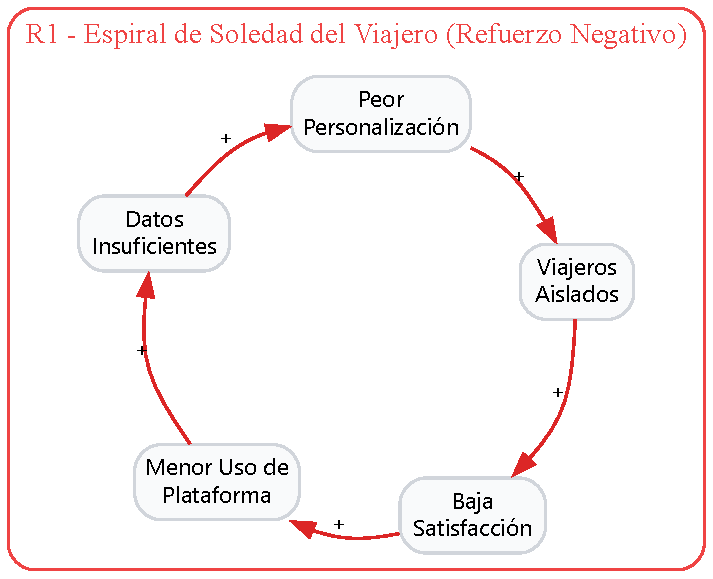
\includegraphics[height=0.3\textheight,keepaspectratio]{../assets/figures/systems.atoms.loneliness-traveler.pdf}
    \caption{Bucle causal R1: Espiral de soledad del viajero}
\end{figure}

Este bucle representa una espiral descendente donde la falta de conexiones sociales reduce la satisfacción del usuario, disminuyendo el uso de la plataforma y limitando la disponibilidad de datos para mejorar los algoritmos de personalización.

\subsubsection{Bucle R2: Fragmentación de Experiencia}

\textbf{Tipo:} Refuerzo Negativo

\textbf{Variables:} Experiencias fragmentadas -> Pérdida de contexto -> Ineficiencia en planificación -> Menor engagement -> Reducida colaboración -> Más fragmentación

\begin{figure}[htbp]
    \centering
    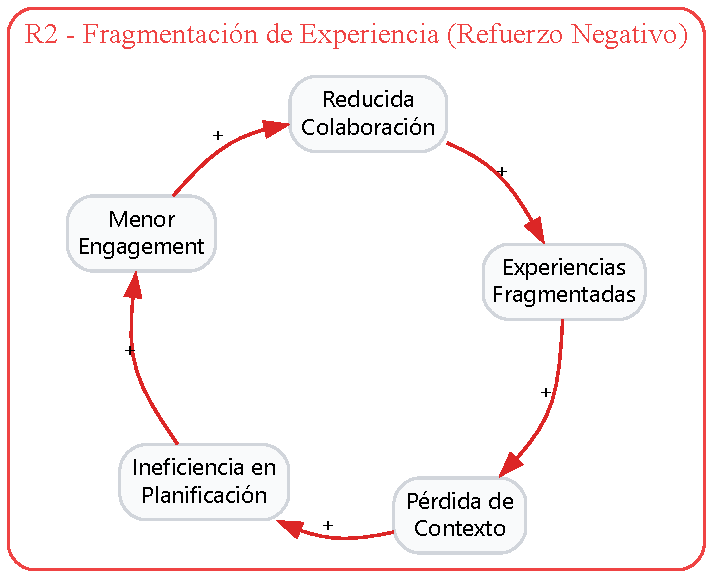
\includegraphics[height=0.3\textheight,keepaspectratio]{../assets/figures/systems.atoms.experience-fragmentation.pdf}
    \caption{Bucle causal R2: Fragmentación de experiencia}
\end{figure}

La separación entre las fases de planificación, ejecución y socialización del viaje genera una pérdida de contexto continuo, reduciendo la efectividad de las conexiones sociales y la colaboración entre viajeros.

\subsubsection{Bucle R3: Limitación de Datos de Matching}

\textbf{Tipo:} Refuerzo Negativo

\textbf{Variables:} Datos limitados -> Algoritmos pobres -> Baja precisión -> Menor confianza -> Menor participación -> Menos datos

\begin{figure}[htbp]
    \centering
    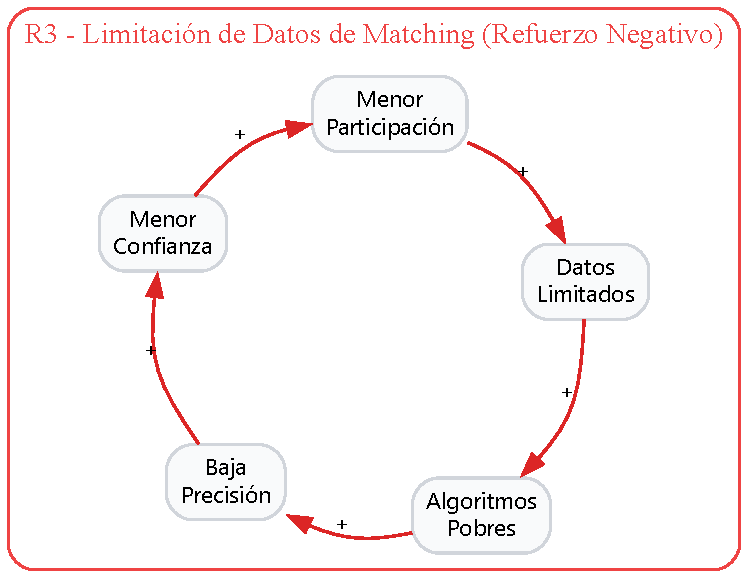
\includegraphics[height=0.3\textheight,keepaspectratio]{../assets/figures/systems.atoms.data-matching-limits.pdf}
    \caption{Bucle causal R3: Limitación de datos de matching}
\end{figure}

La escasez de datos sociales limita la efectividad de los algoritmos de matching, creando un ciclo de desconfianza que reduce la participación de los usuarios y perpetúa la limitación de datos.

\subsubsection{Bucle B1: Escalabilidad de Personalización}

\textbf{Tipo:} Balanceo

\textbf{Variables:} Complejidad de matching -> Recursos computacionales -> Tiempo de respuesta -> Experiencia usuario -> Adopción -> Limitación escala

\begin{figure}[htbp]
    \centering
    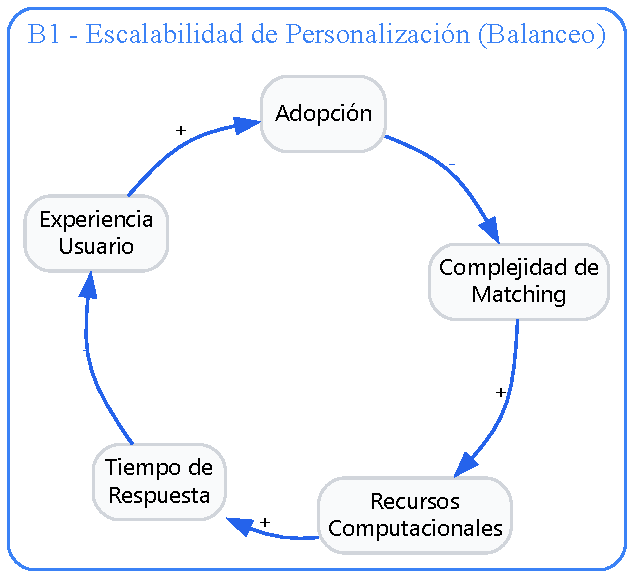
\includegraphics[height=0.3\textheight,keepaspectratio]{../assets/figures/systems.atoms.personalization-scaling.pdf}
    \caption{Bucle causal B1: Escalabilidad de personalización}
\end{figure}

La complejidad computacional del matching multidimensional crea restricciones de rendimiento que afectan la experiencia del usuario y limitan la adopción masiva de la plataforma.

\subsubsection{Bucle R4: Validación Social Post-Viaje}

\textbf{Tipo:} Refuerzo Positivo

\textbf{Variables:} Experiencias compartidas -> Datos de validación -> Mejora de algoritmos -> Mejor matching -> Más experiencias exitosas

\begin{figure}[htbp]
    \centering
    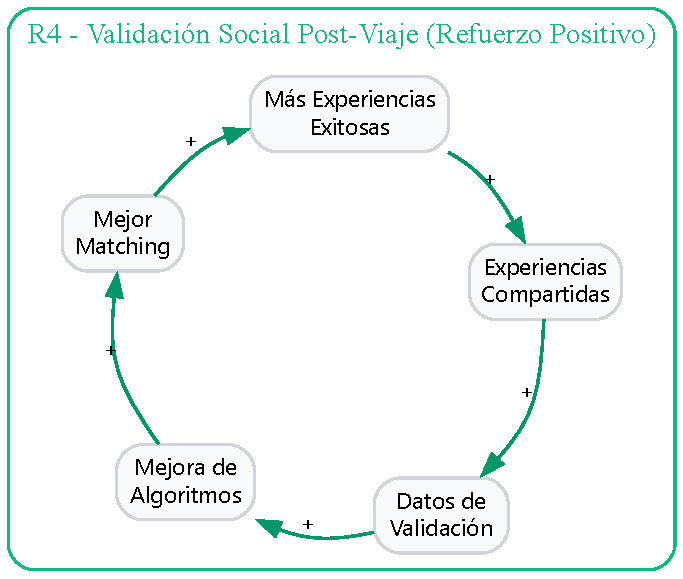
\includegraphics[height=0.3\textheight,keepaspectratio]{../assets/figures/systems.atoms.post-trip-social-validation.pdf}
    \caption{Bucle causal R4: Validación social post-viaje}
\end{figure}

Este bucle positivo representa el potencial de crecimiento del sistema mediante el aprendizaje continuo de experiencias compartidas, mejorando progresivamente la calidad del matching y generando más experiencias exitosas.

\subsection{Arquetipos Sistémicos Identificados}

El análisis revela cuatro arquetipos sistémicos principales que gobiernan el comportamiento del sistema turístico digital:

\subsubsection{Límites del Crecimiento}

El sistema exhibe un claro arquetipo de ``Límites del Crecimiento'' donde el bucle de refuerzo positivo R4 impulsa el crecimiento inicial a través de experiencias exitosas, pero se encuentra con múltiples límites que frenan este crecimiento:

\begin{itemize}
\item \textbf{Límite principal (R1):} La espiral de soledad del viajero crea un ciclo vicioso que reduce la satisfacción y el uso de la plataforma
\item \textbf{Límite de datos (R3):} La limitación de datos de matching crea una barrera fundamental para la personalización efectiva
\item \textbf{Límite técnico (B1):} La escalabilidad de personalización introduce restricciones computacionales que afectan la experiencia del usuario
\end{itemize}

\subsubsection{Desplazamiento de la Carga}

Se observa un patrón de ``Desplazamiento de la Carga'' donde la solución sintomática (R4 - Validación Social Post-Viaje) alivia temporalmente los síntomas pero debilita la capacidad del sistema para resolver el problema fundamental:

\begin{itemize}
\item \textbf{Solución sintomática:} R4 proporciona validación social y mejora temporal de matching
\item \textbf{Problema fundamental:} R1 (Soledad del Viajero) y R2 (Fragmentación de Experiencia) representan las causas raíz
\item \textbf{Efecto secundario:} La dependencia en R4 reduce la motivación para abordar los problemas estructurales
\end{itemize}

\subsubsection{Erosión de Metas}

El sistema muestra erosión gradual de las metas originales a través de la degradación progresiva de estándares:

\begin{itemize}
\item \textbf{Meta original:} Proporcionar experiencias de viaje personalizadas y conectadas
\item \textbf{Erosión:} R1 y R3 degradan progresivamente la calidad de la experiencia y personalización
\item \textbf{Aceptación del deterioro:} B1 muestra cómo el sistema se adapta a limitaciones técnicas aceptando estándares menores
\end{itemize}

\subsubsection{Éxito a los Exitosos}

Se crea una brecha creciente entre usuarios exitosos y usuarios en dificultades:

\begin{itemize}
\item \textbf{Ganadores:} Usuarios que participan en R4 obtienen mejores experiencias y más matching
\item \textbf{Perdedores:} Usuarios atrapados en R1 y R2 reciben servicios degradados
\item \textbf{Reforzamiento:} R4 mejora los algoritmos para los ya exitosos, mientras que R1 y R3 empeoran para los marginados
\end{itemize}

\subsection{Puntos de Apalancamiento del Sistema}

El análisis sistémico identifica tres puntos de apalancamiento de alto impacto para intervenir efectivamente en el sistema:

\subsubsection{Intervención en Datos de Matching (R3)}

\textbf{Impacto:} Afecta directamente R1, R4 y B1

\textbf{Estrategia:} Implementar estrategias de adquisición de datos y participación

\textbf{Resultado esperado:} Mejora general del sistema y rompe múltiples ciclos negativos

\subsubsection{Integración de Experiencias (R2)}

\textbf{Impacto:} Reduce fragmentación y facilita conexiones sociales

\textbf{Estrategia:} Diseñar flujos integrados que promuevan colaboración natural

\textbf{Resultado esperado:} Ataca directamente la soledad y mejora engagement

\subsubsection{Optimización de Algoritmos (R4 × B1)}

\textbf{Impacto:} Balancea crecimiento con sostenibilidad técnica

\textbf{Estrategia:} Desarrollar algoritmos eficientes que escalen bien

\textbf{Resultado esperado:} Sostenibilidad del crecimiento a largo plazo

\begin{figure}[htbp]
    \centering
    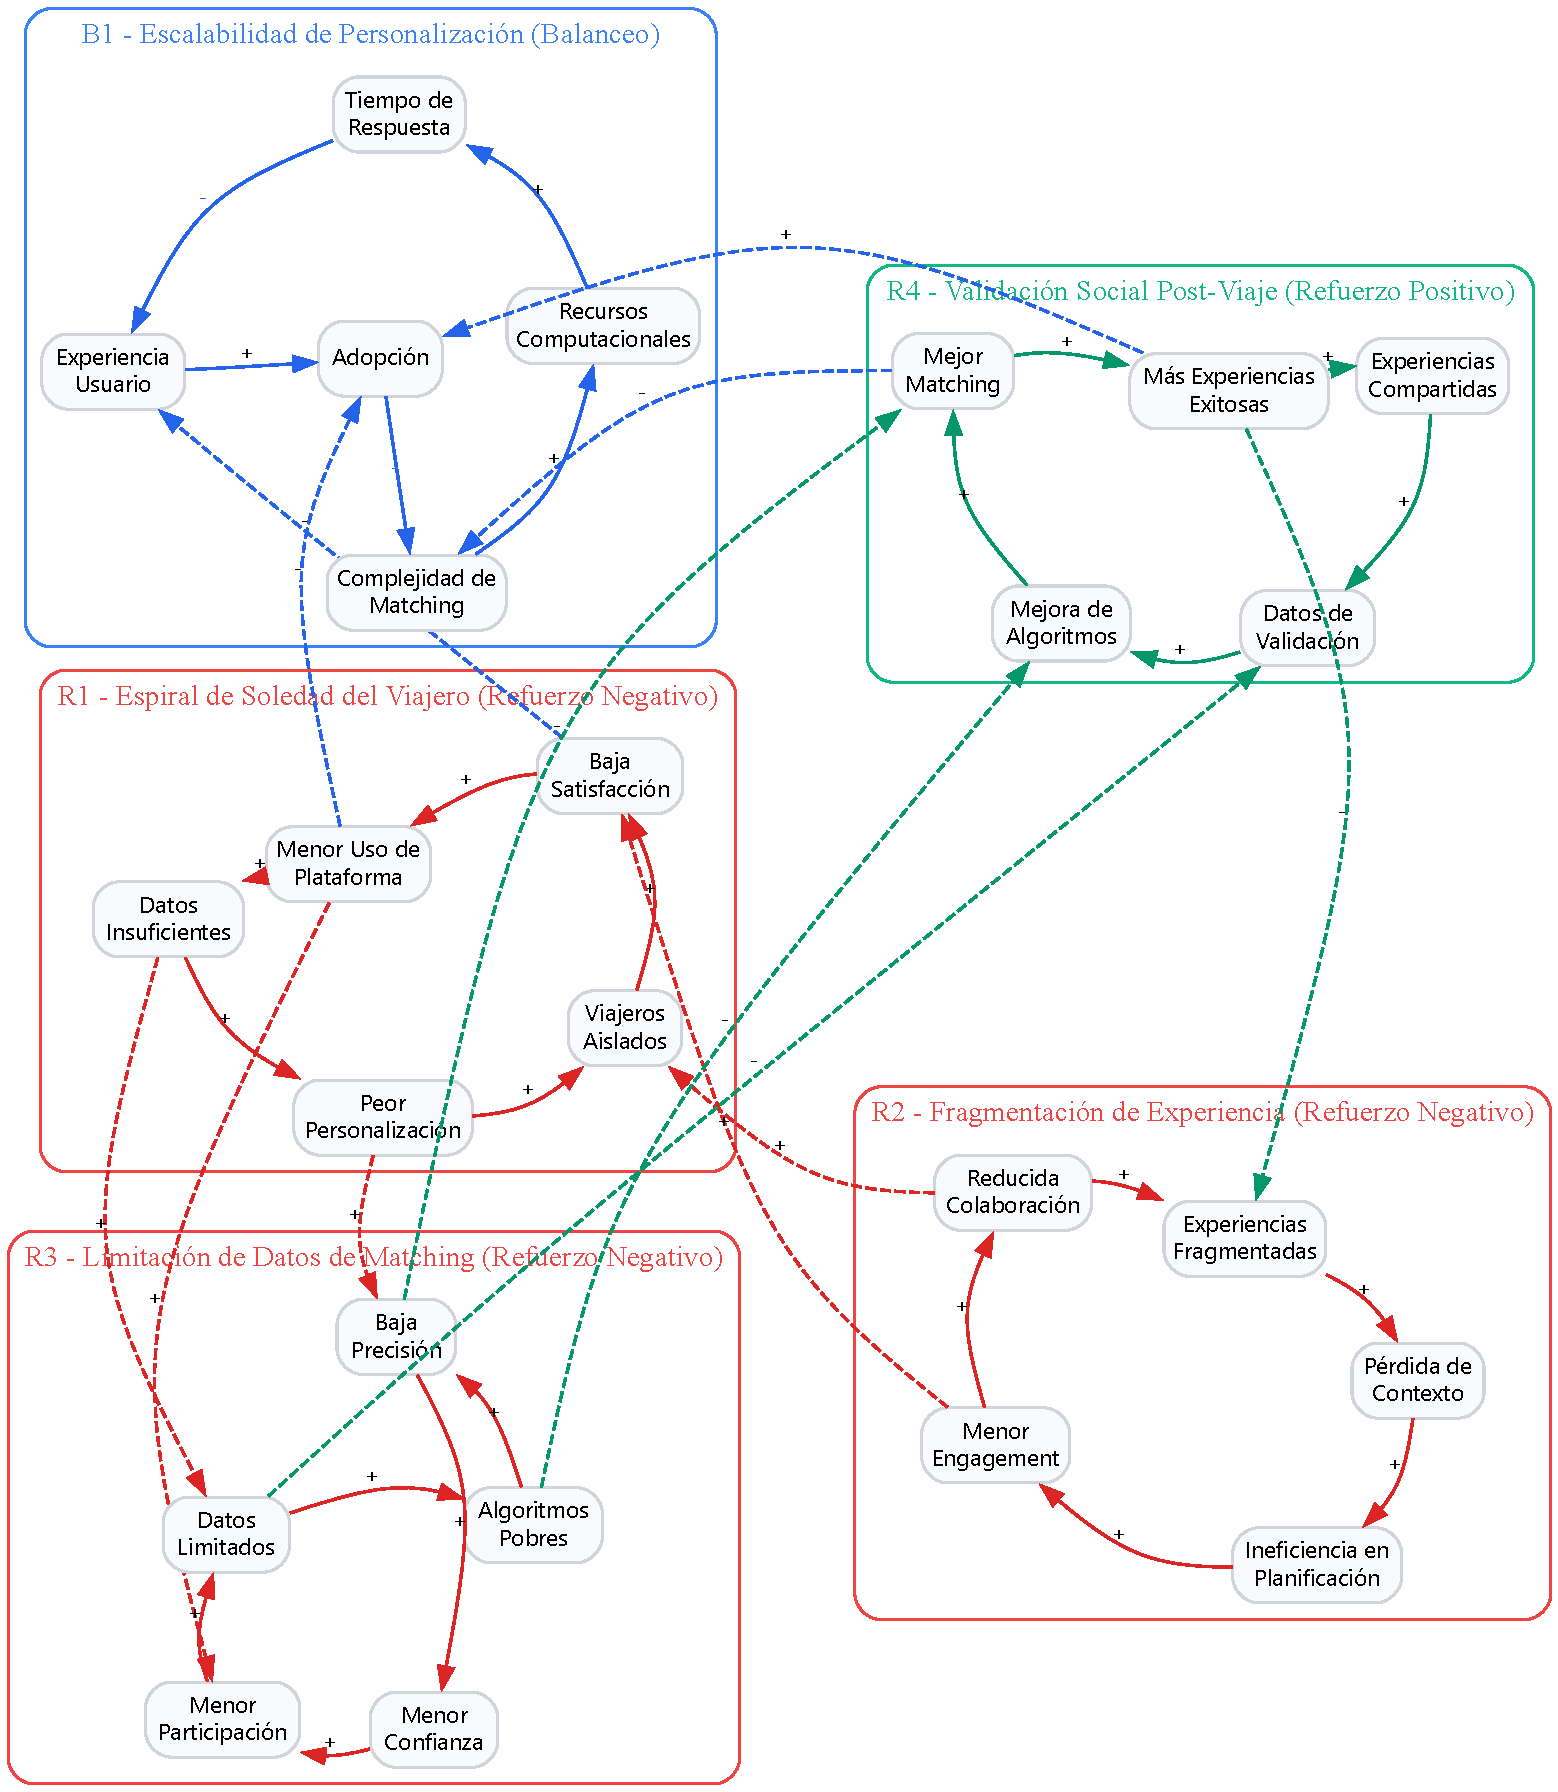
\includegraphics[width=0.9\linewidth,height=0.5\textheight,keepaspectratio]{../assets/figures/systems.maps.systemic-model.pdf}
    \caption{Modelo sistémico integrado con interacciones entre bucles causales}
\end{figure}

\subsection{Implicaciones Estratégicas para la Transformación Digital}

El análisis sistémico proporciona insights estratégicos cruciales para la implementación exitosa de la transformación digital:

\subsubsection{Enfoque en Causa Raíz}

Abordar aislamiento (R1) y fragmentación (R2) en lugar de solo optimización algorítmica superficial. Las intervenciones deben centrarse en:

\begin{itemize}
\item Programas de onboarding que prevengan el aislamiento inicial
\item Flujos de trabajo integrados que mantengan contexto continuo
\item Mecanismos de conexión natural entre usuarios
\end{itemize}

\subsubsection{Estrategia de Datos}

Priorizar adquisición de datos y participación para romper restricciones R3:

\begin{itemize}
\item Incentivos para compartir experiencias y preferencias
\item Mecanismos de validación social que generen datos de calidad
\item Procesamiento de datos que mejore progresivamente los algoritmos
\end{itemize}

\subsubsection{Crecimiento Sostenible}

Balancear expansión R4 con limitaciones técnicas B1:

\begin{itemize}
\item Optimización algorítmica para reducir complejidad computacional
\item Arquitectura escalable que soporte crecimiento sostenible
\item Métricas de calidad que detecten erosión de metas
\end{itemize}

\subsection{Recomendaciones de Intervención}

\subsubsection{Prioridad Alta: Romper Ciclos de Refuerzo Negativo}

\begin{enumerate}
\item \textbf{Implementar programas de onboarding} que prevengan el aislamiento inicial (R1)
\item \textbf{Crear incentivos de participación} para aumentar datos disponibles (R3)
\item \textbf{Diseñar experiencias integradas} que faciliten colaboración natural (R2)
\end{enumerate}

\subsubsection{Prioridad Media: Optimizar Crecimiento Positivo}

\begin{enumerate}
\item \textbf{Mejorar eficiencia algorítmica} para sostener R4 sin sobrecargar B1
\item \textbf{Desarrollar mecanismos de redistribución} para evitar ``éxito a los exitosos''
\item \textbf{Establecer métricas de calidad} para detectar erosión de metas
\end{enumerate}

%================================================================================
\section{Diagramas de Arquitectura (C4 Model)}
%================================================================================

Los diagramas C4 ilustran el sistema como conjunto de contenedores y relaciones; deben interpretarse de manera consistente con la topología del repositorio de infraestructura: clientes web y móvil, API Gateway, balanceador de aplicaciones, dos servicios de cómputo (Spring Boot y FastAPI), RDS PostgreSQL, S3, SNS/SQS y CloudFront/CloudWatch según corresponda.

Para evitar el uso decorativo de diagramas, en esta sección cada vista se interpreta con tres preguntas: \textbf{(i)} ¿qué decisión arquitectónica justifica?, \textbf{(ii)} ¿qué riesgo reduce?, y \textbf{(iii)} ¿qué métrica posterior permite evaluar? Este criterio se aplica de forma homogénea a C4, ArchiMate y UML.

\subsection*{Lectura analítica por niveles}

\textbf{Nivel de contexto (C4 L1 y contexto UML):} Delimita frontera de sistema y actores externos. La decisión principal es centralizar el ingreso por perímetro API para reducir acoplamiento cliente-proveedor. El riesgo mitigado es la integración punto a punto no gobernada. Métrica asociada: tasa de fallos de integración por canal.

\textbf{Nivel de contenedores (C4 L2):} Justifica separación de responsabilidades entre capa de experiencia, backend transaccional, servicio de IA, persistencia y mensajería. El riesgo mitigado es el escalamiento acoplado de cargas heterogéneas. Métrica asociada: latencia p95 por contenedor y uso de CPU por dominio.

\textbf{Nivel de componentes (C4 L3, componentes UML y ER):} Conecta funcionalidades con módulos concretos y estructuras de datos. El riesgo mitigado es ambigüedad de ownership técnico. Métrica asociada: cobertura de pruebas por componente crítico y defectos por módulo.

\textbf{Nivel de despliegue/operación (UML deployment, red y CI/CD):} Establece trazabilidad desde diseño lógico hasta ejecución en nube y cadena de entrega. El riesgo mitigado es divergencia entre arquitectura documentada y arquitectura desplegada. Métrica asociada: tiempo de despliegue, tasa de rollback y MTTR.

\begin{figure}[htbp]
    \centering
    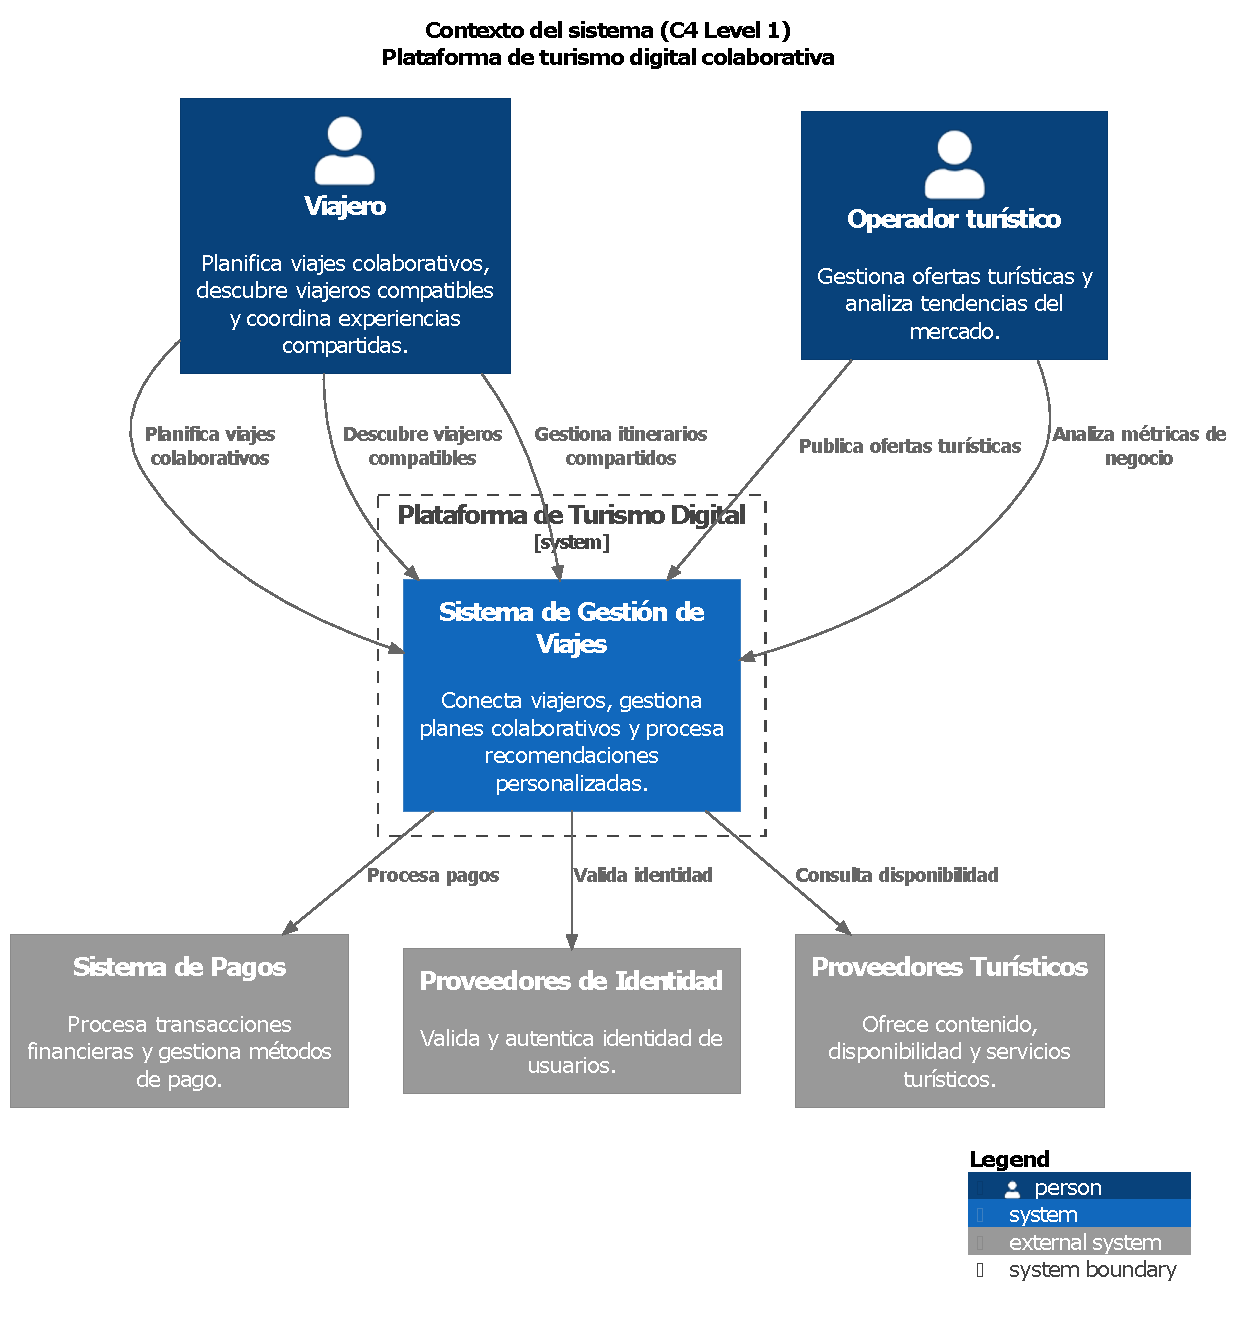
\includegraphics[width=0.9\linewidth,height=0.52\textheight,keepaspectratio]{../assets/figures/c4-model.level-1-context.pdf}
    \caption{Diagrama de contexto C4 (alineación con API Gateway, ALB y servicios de cómputo documentados)}
\end{figure}
\noindent\textit{Explicación:} Este diagrama delimita la frontera del sistema y confirma que las integraciones externas se concentran en un perímetro controlado, reduciendo acoplamiento punto a punto.

\begin{figure}[htbp]
    \centering
    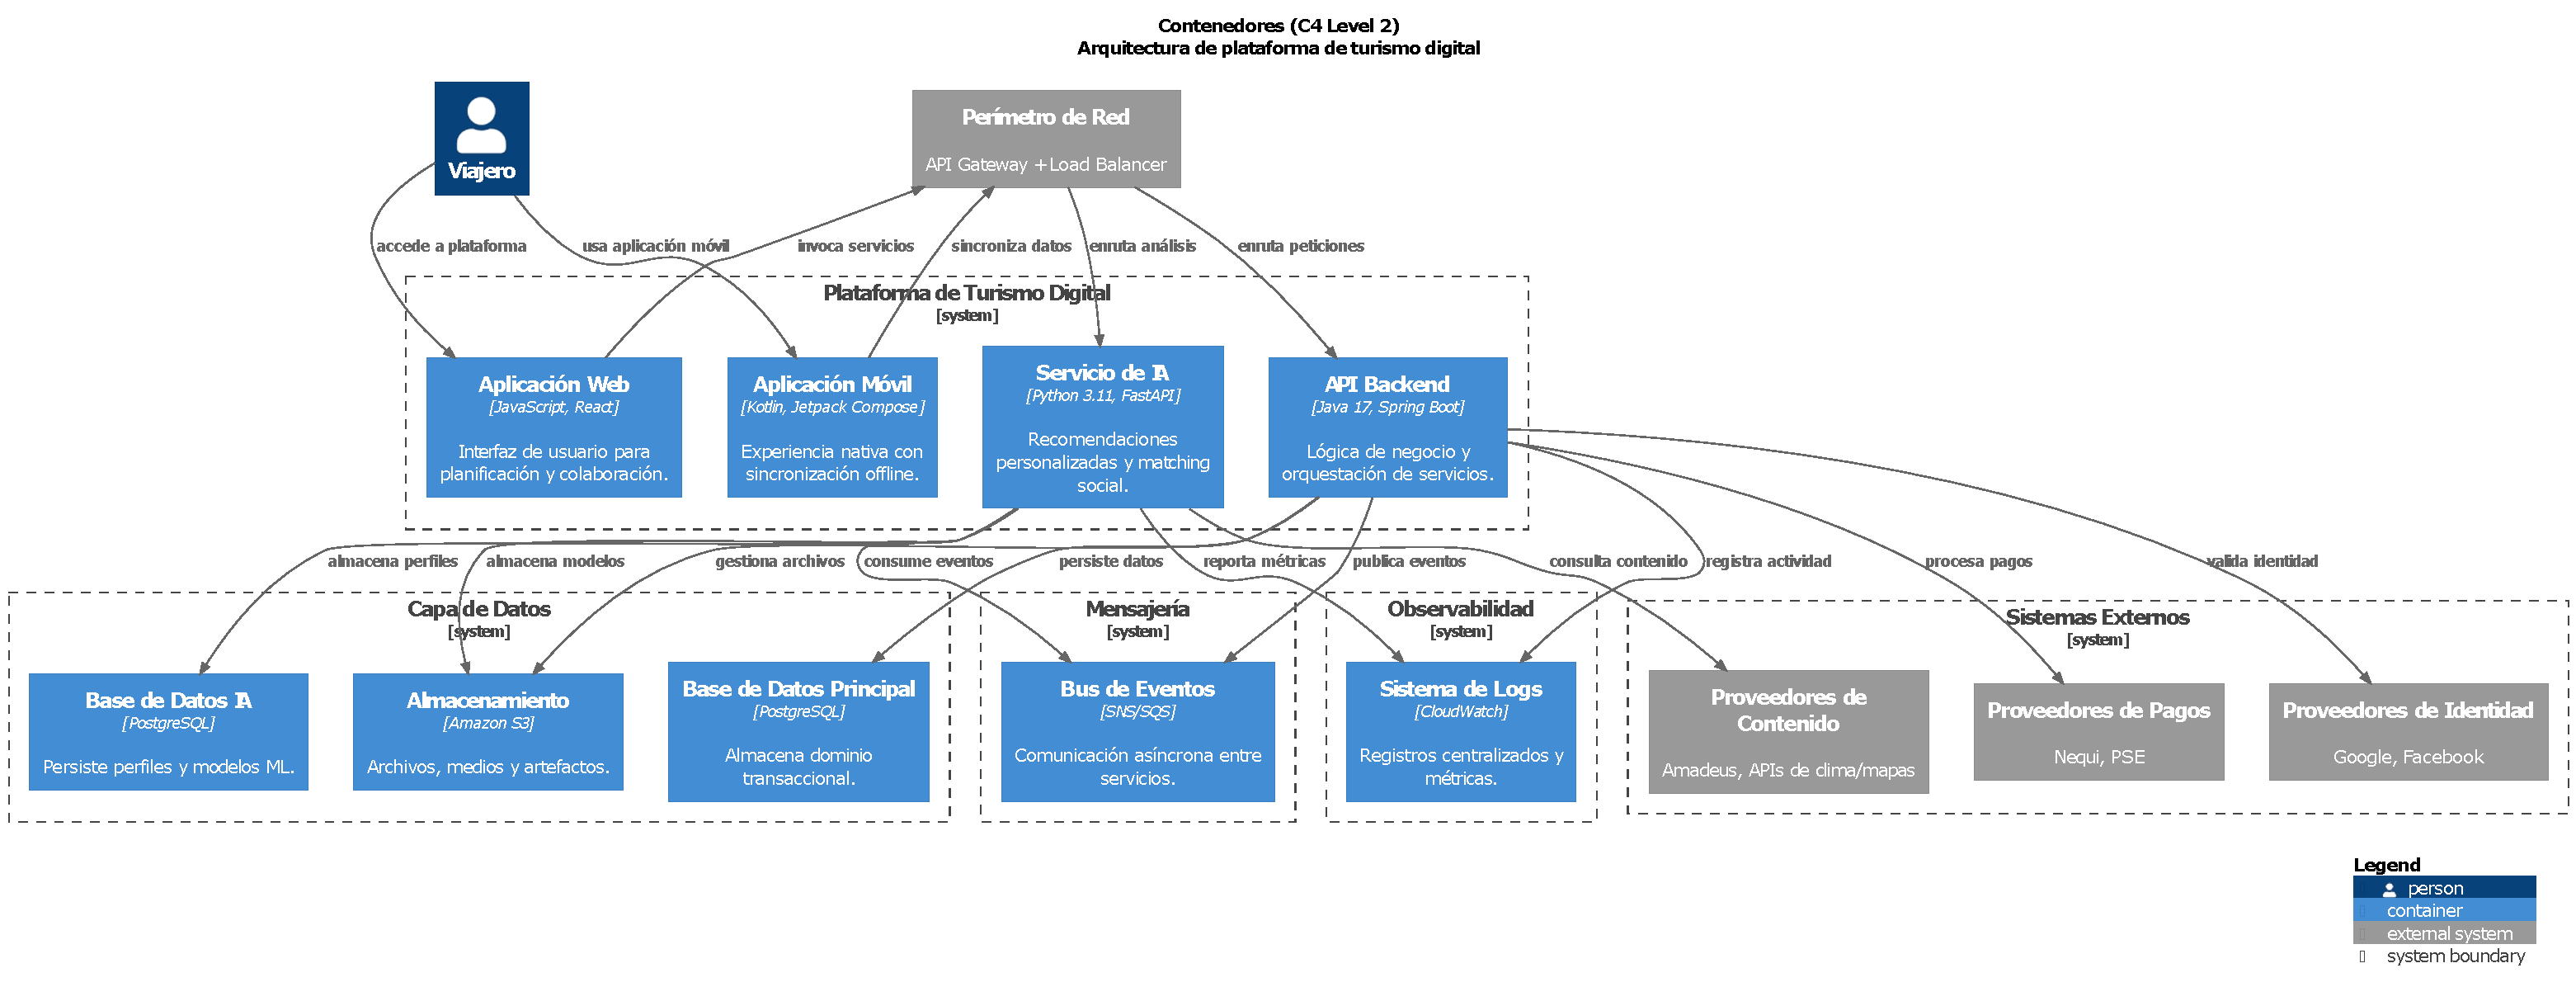
\includegraphics[width=0.9\linewidth,height=0.52\textheight,keepaspectratio]{../assets/figures/c4-model.level-2-containers.pdf}
    \caption{Diagrama de contenedores C4 (núcleo backend, microservicio IA, persistencia y mensajería)}
\end{figure}
\noindent\textit{Explicación:} La vista de contenedores evidencia separación de responsabilidades por dominio y sustenta escalabilidad independiente entre cargas transaccionales y de IA.

\begin{figure}[htbp]
    \centering
    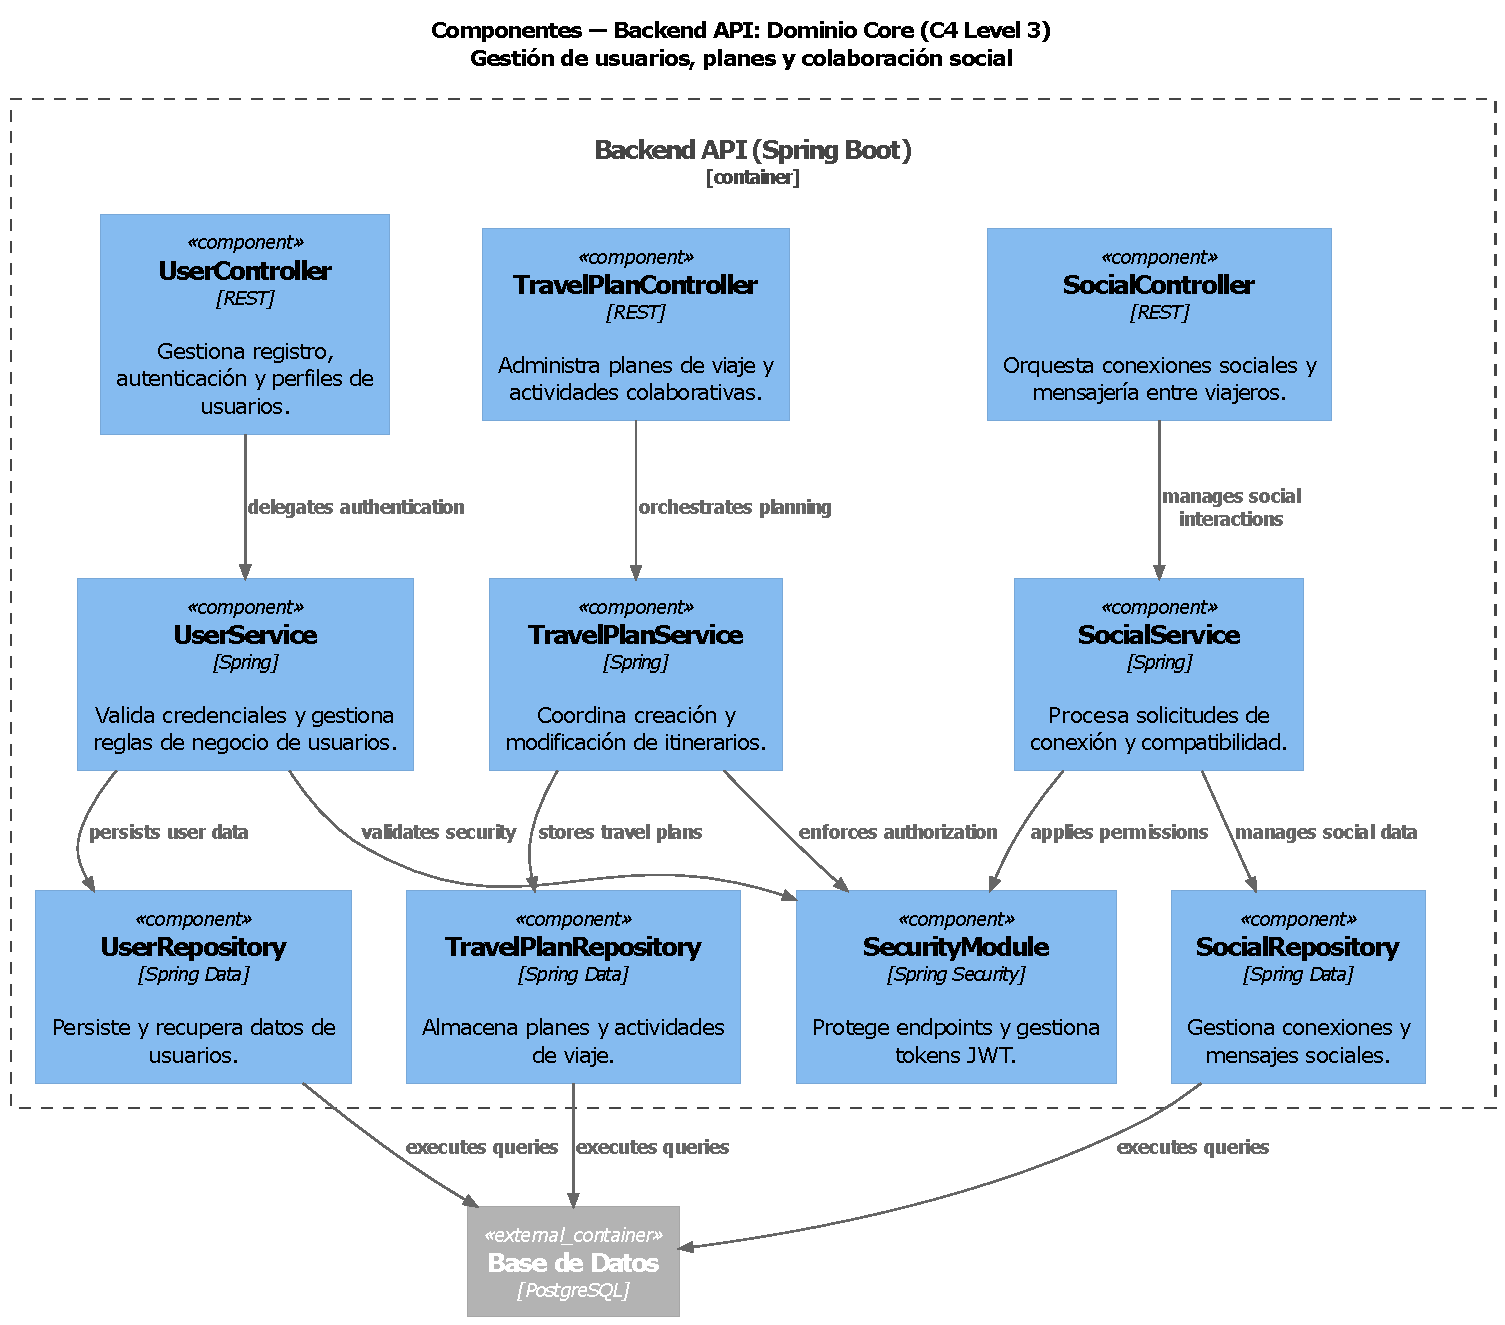
\includegraphics[width=0.88\linewidth,height=0.5\textheight,keepaspectratio]{../assets/figures/c4-model.level-3-components.backend.core.pdf}
    \caption{Diagrama de componentes del backend core (Spring Boot)}
\end{figure}
\noindent\textit{Explicación:} El backend core concentra reglas de negocio y consistencia transaccional, con interfaces explícitas para controladores, servicios y persistencia.

\begin{figure}[htbp]
    \centering
    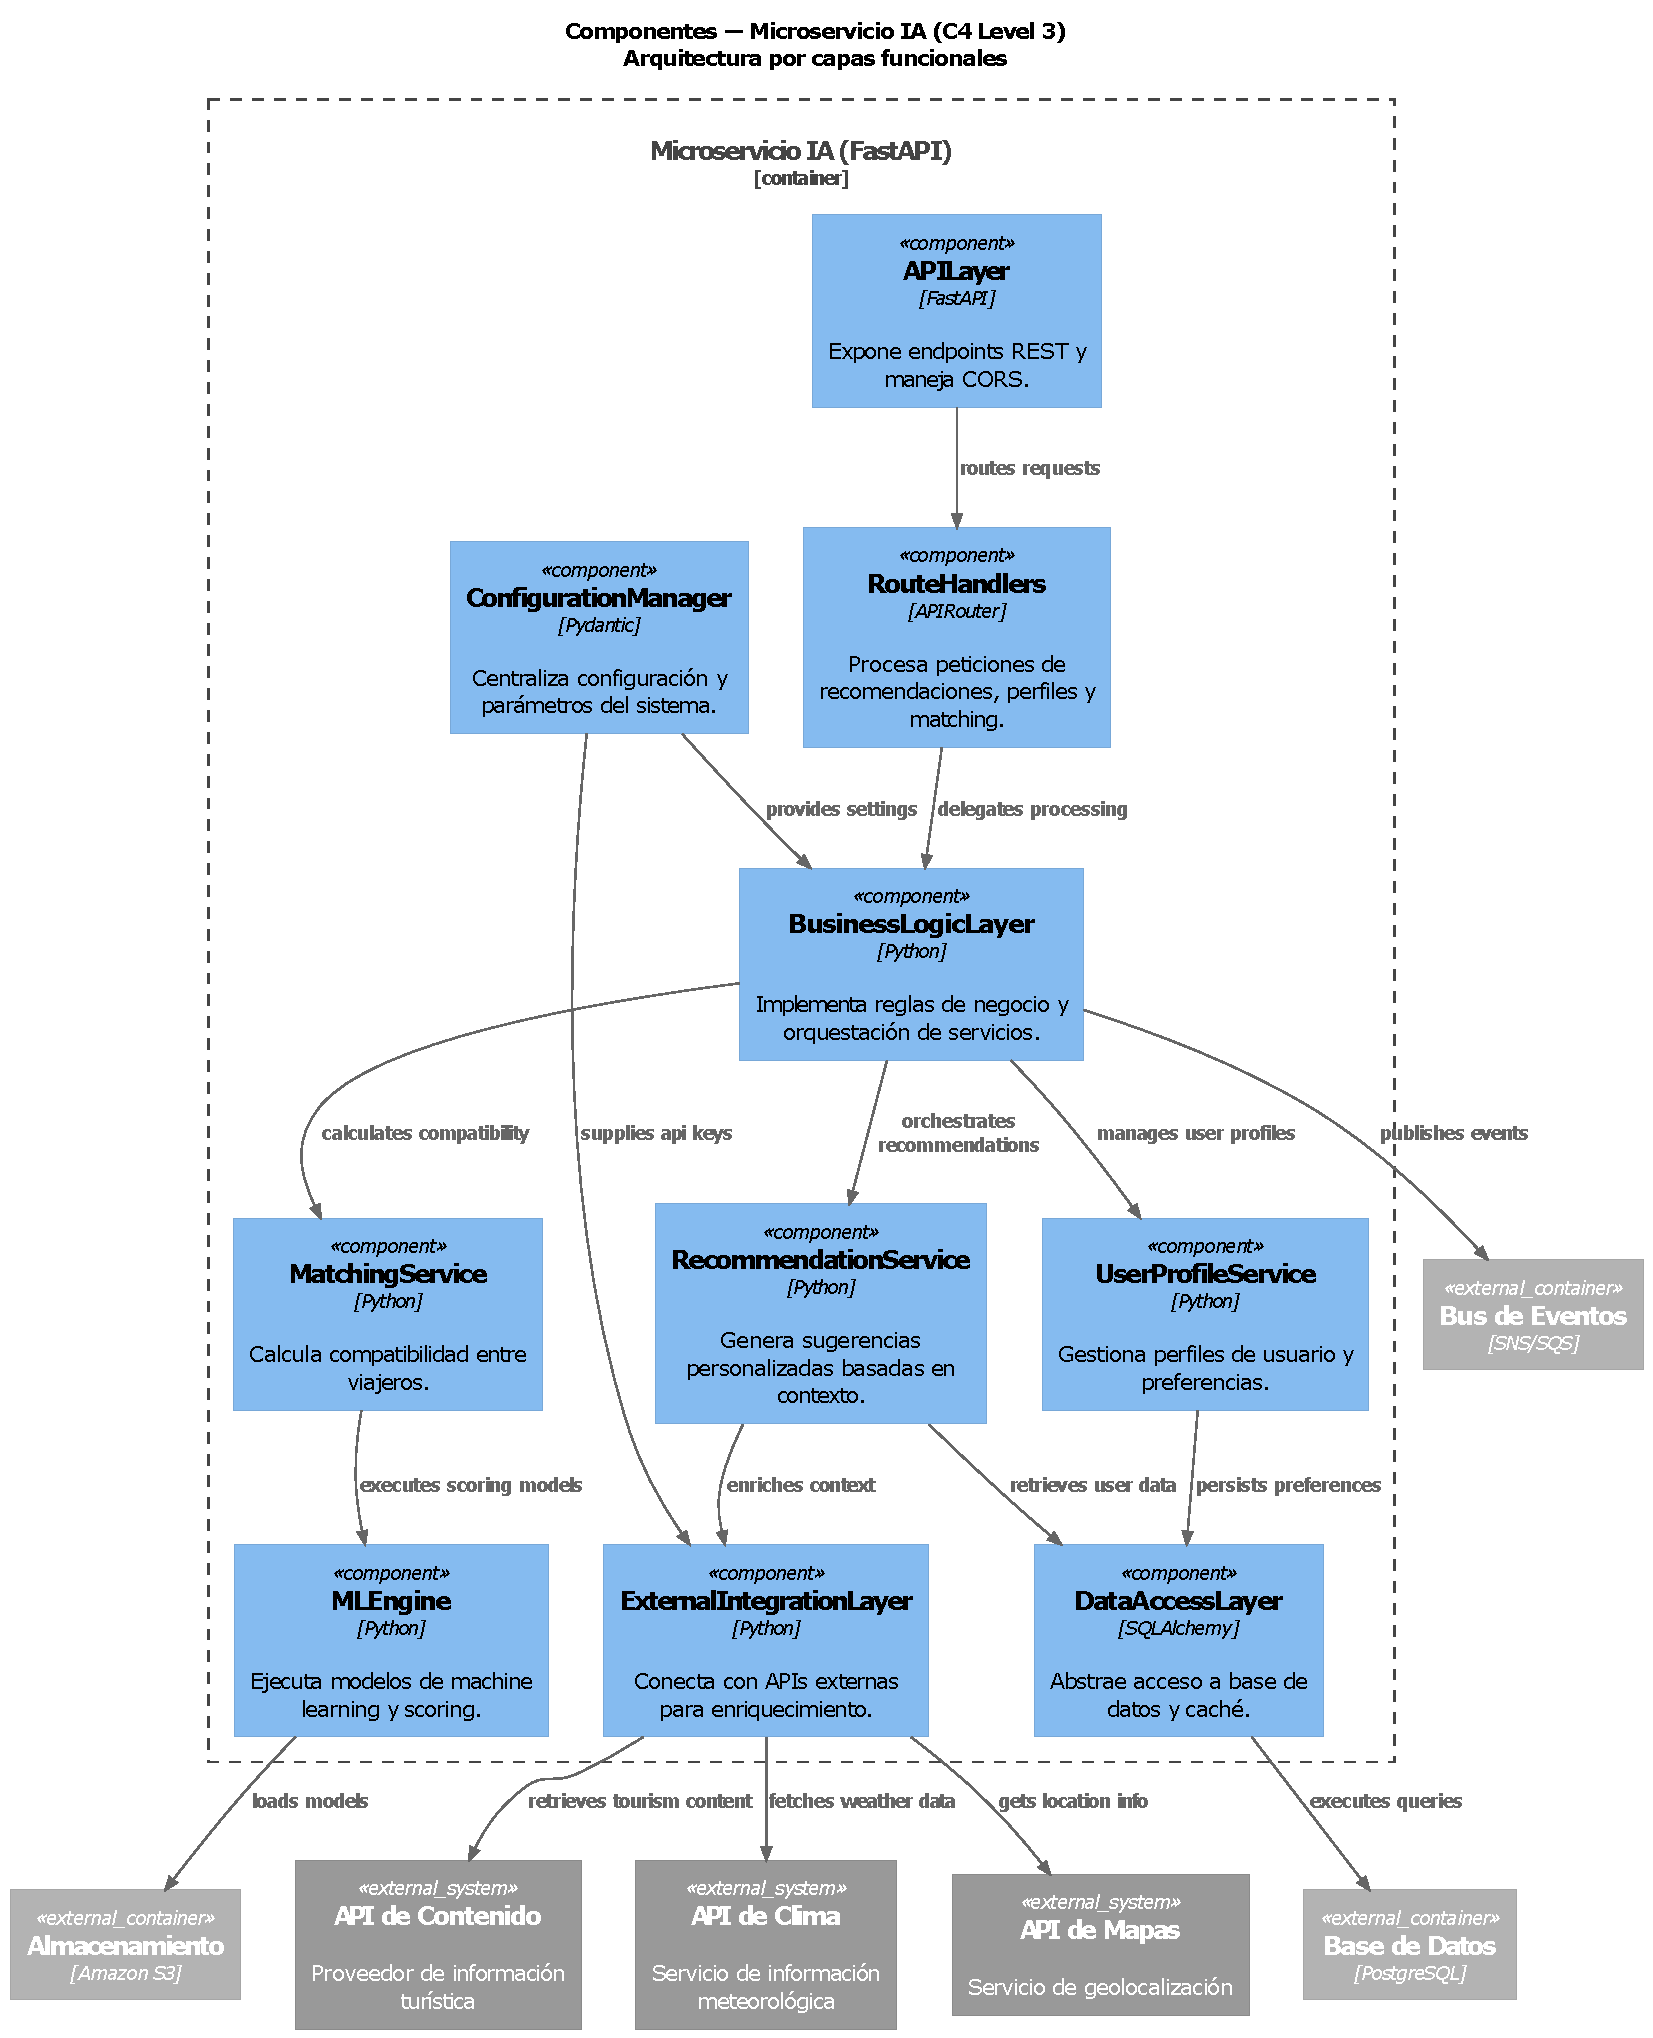
\includegraphics[width=0.88\linewidth,height=0.5\textheight,keepaspectratio]{../assets/figures/c4-model.level-3-components.ai-microservice.pdf}
    \caption{Diagrama de componentes del microservicio de IA (FastAPI)}
\end{figure}
\noindent\textit{Explicación:} El microservicio de IA encapsula inferencia y lógica de recomendación, reduciendo impacto de cambios algorítmicos sobre el núcleo transaccional.

\begin{figure}[htbp]
    \centering
    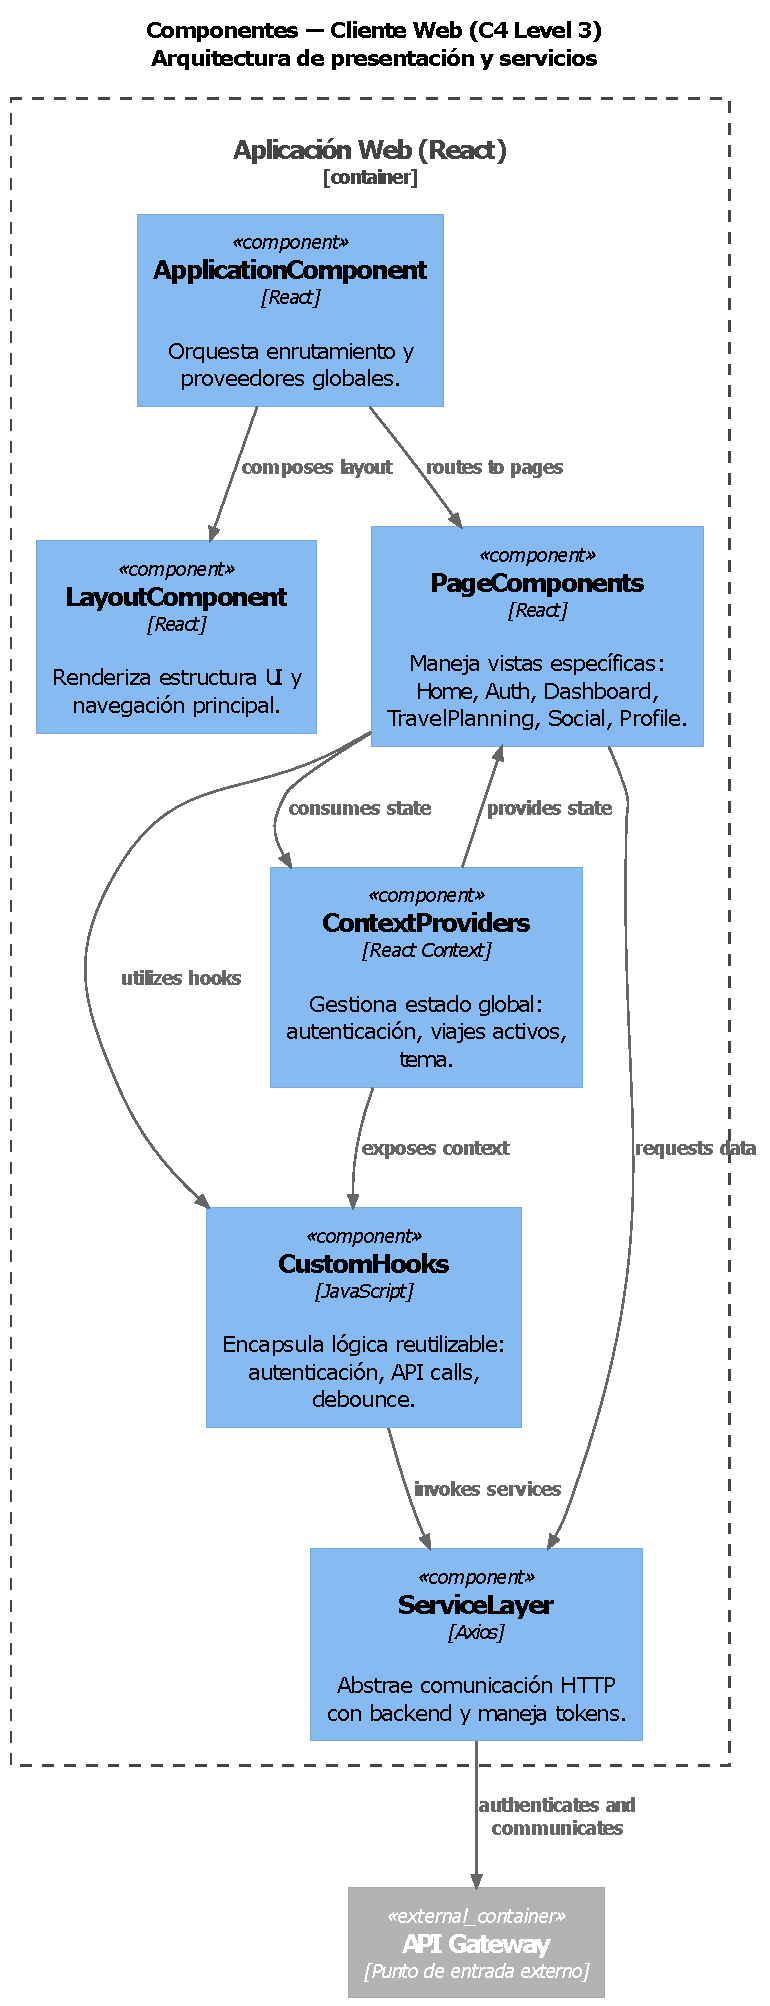
\includegraphics[width=0.88\linewidth,height=0.5\textheight,keepaspectratio]{../assets/figures/c4-model.level-3-components.web-client.pdf}
    \caption{Diagrama de componentes del cliente web (React)}
\end{figure}
\noindent\textit{Explicación:} El cliente web organiza presentación, estado y consumo de APIs, facilitando mantenibilidad y evolución de experiencia de usuario.

\begin{figure}[htbp]
    \centering
    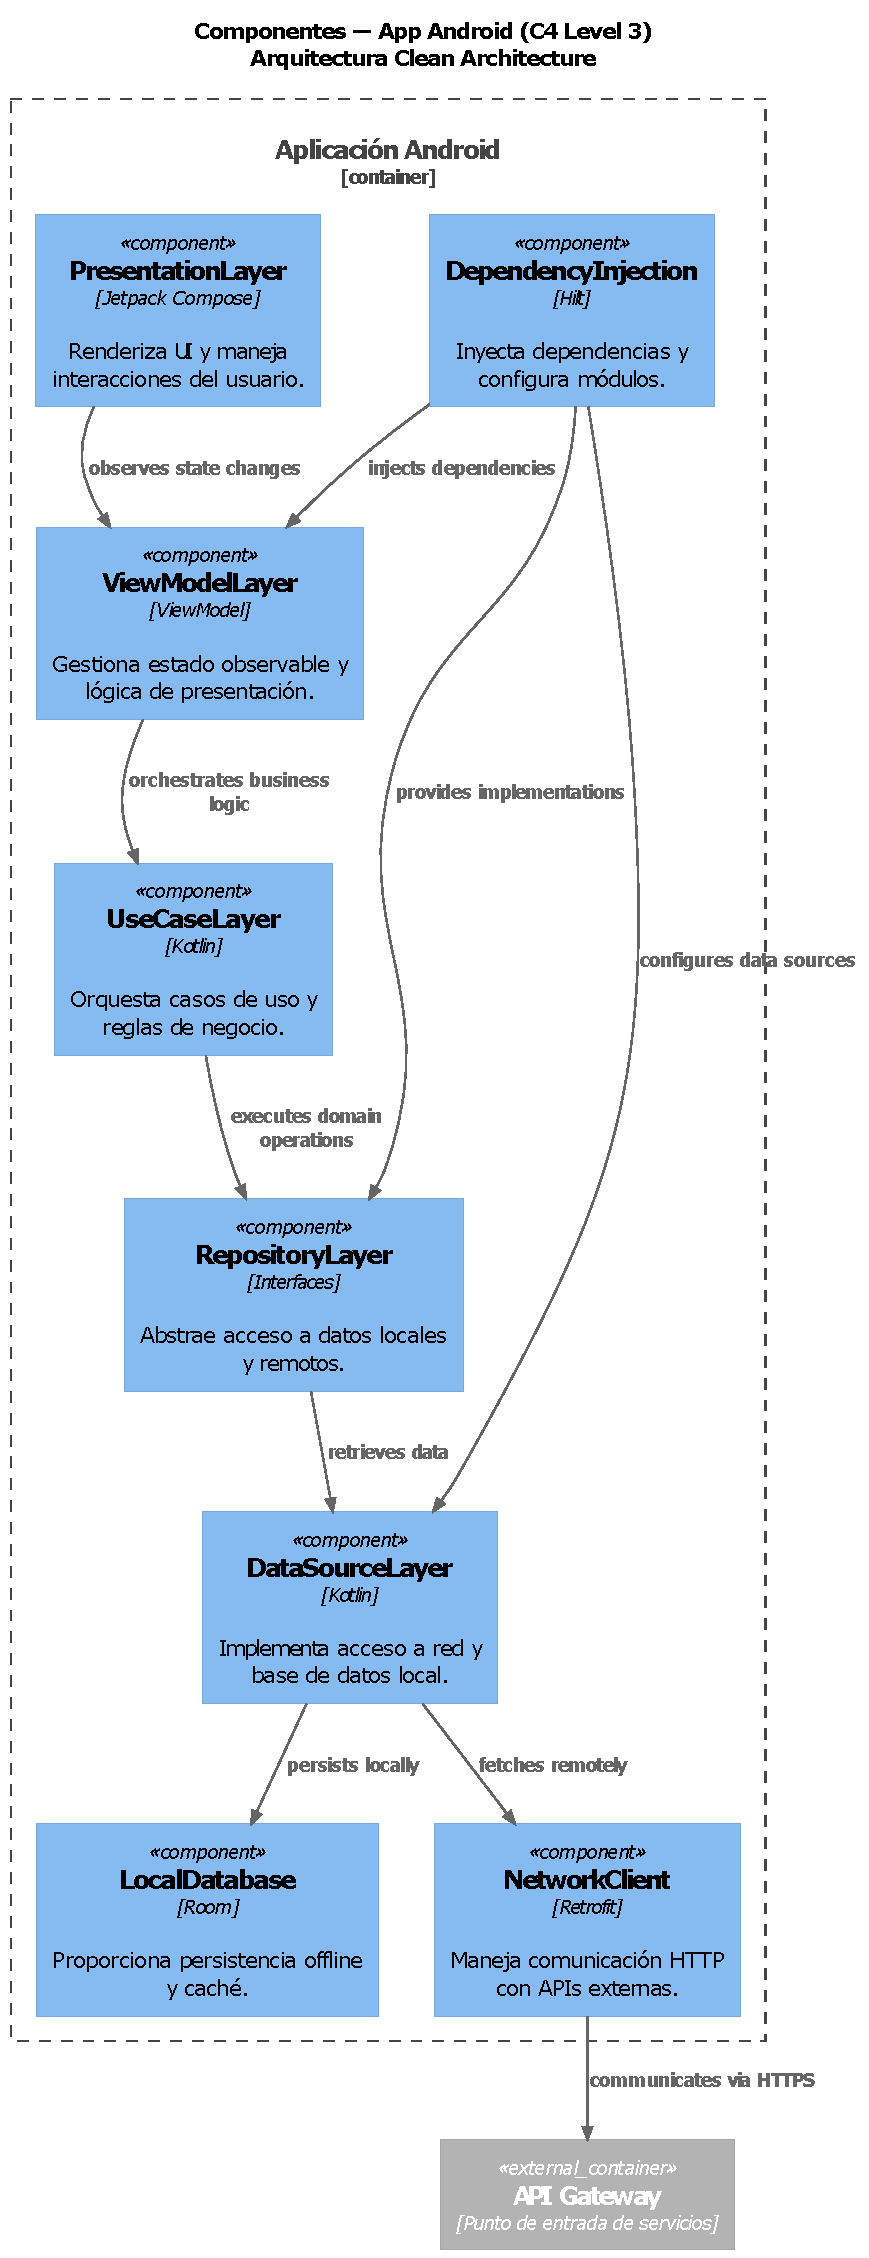
\includegraphics[width=0.88\linewidth,height=0.5\textheight,keepaspectratio]{../assets/figures/c4-model.level-3-components.android-app.pdf}
    \caption{Diagrama de componentes del cliente móvil (Android/Kotlin)}
\end{figure}
\noindent\textit{Explicación:} La arquitectura móvil muestra separación de capas y soporte de sincronización, clave para operación en escenarios de conectividad variable.

\begin{figure}[htbp]
    \centering
    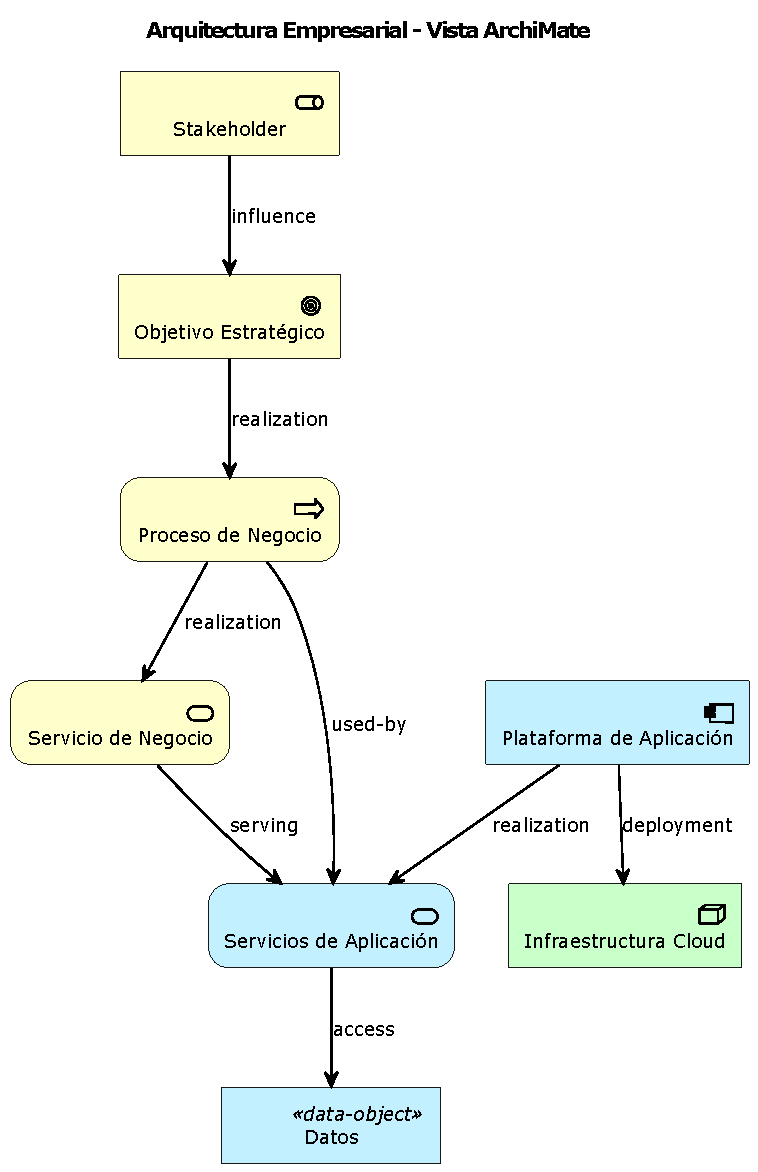
\includegraphics[width=0.9\linewidth,height=0.55\textheight,keepaspectratio]{../assets/figures/enterprise.archimate.pdf}
    \caption{Diagrama de arquitectura empresarial (ArchiMate)}
\end{figure}
\noindent\textit{Explicación:} Esta vista alinea objetivos de negocio, procesos y activos tecnológicos, asegurando trazabilidad entre estrategia y ejecución técnica.

\begin{figure}[htbp]
    \centering
    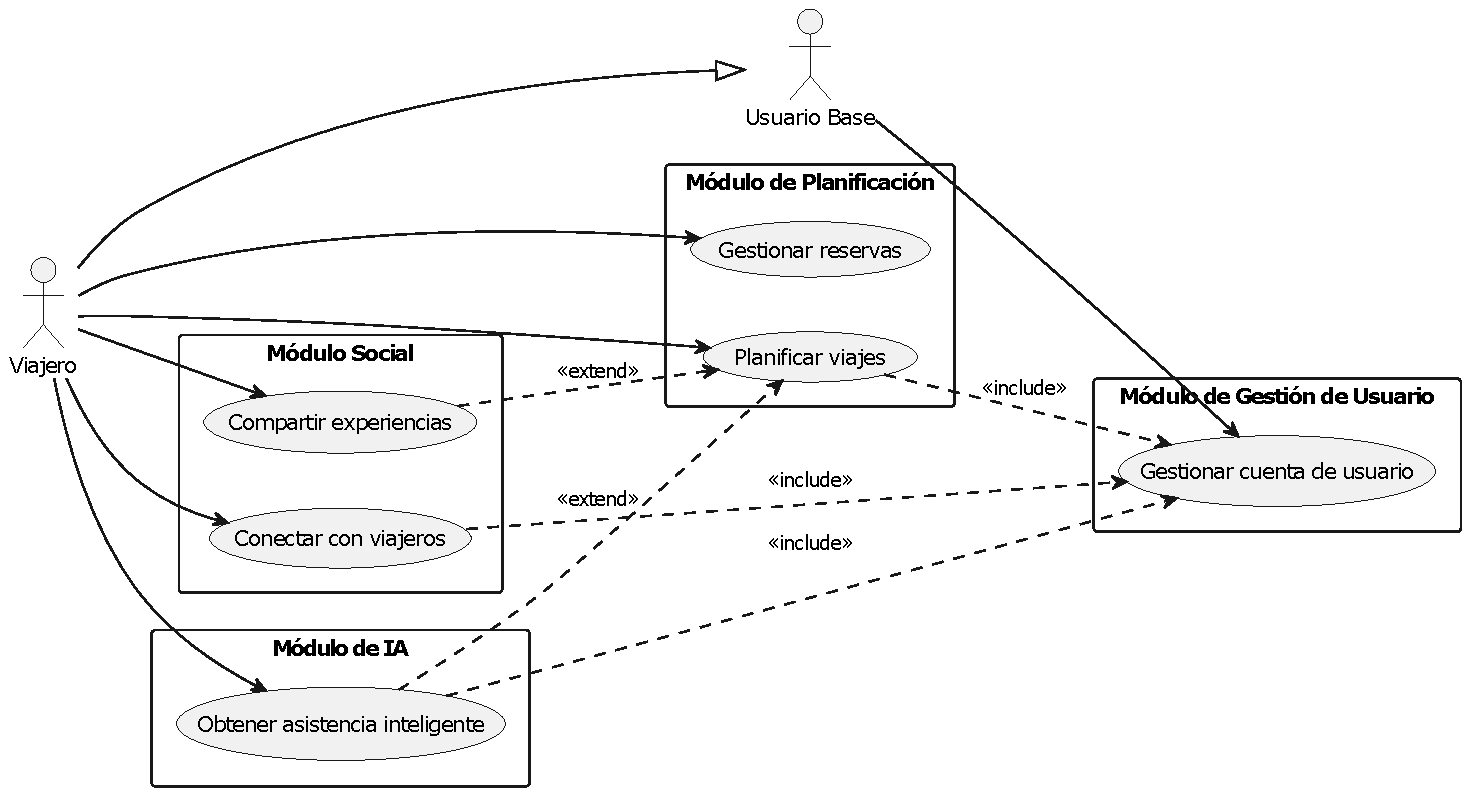
\includegraphics[width=0.9\linewidth,height=0.52\textheight,keepaspectratio]{../assets/figures/uml.behavior.use-cases.pdf}
    \caption{Diagrama de casos de uso del sistema}
\end{figure}
\noindent\textit{Explicación:} El diagrama identifica interacciones principales del usuario con la plataforma y delimita el alcance funcional evaluado en el prototipo.

\begin{figure}[htbp]
    \centering
    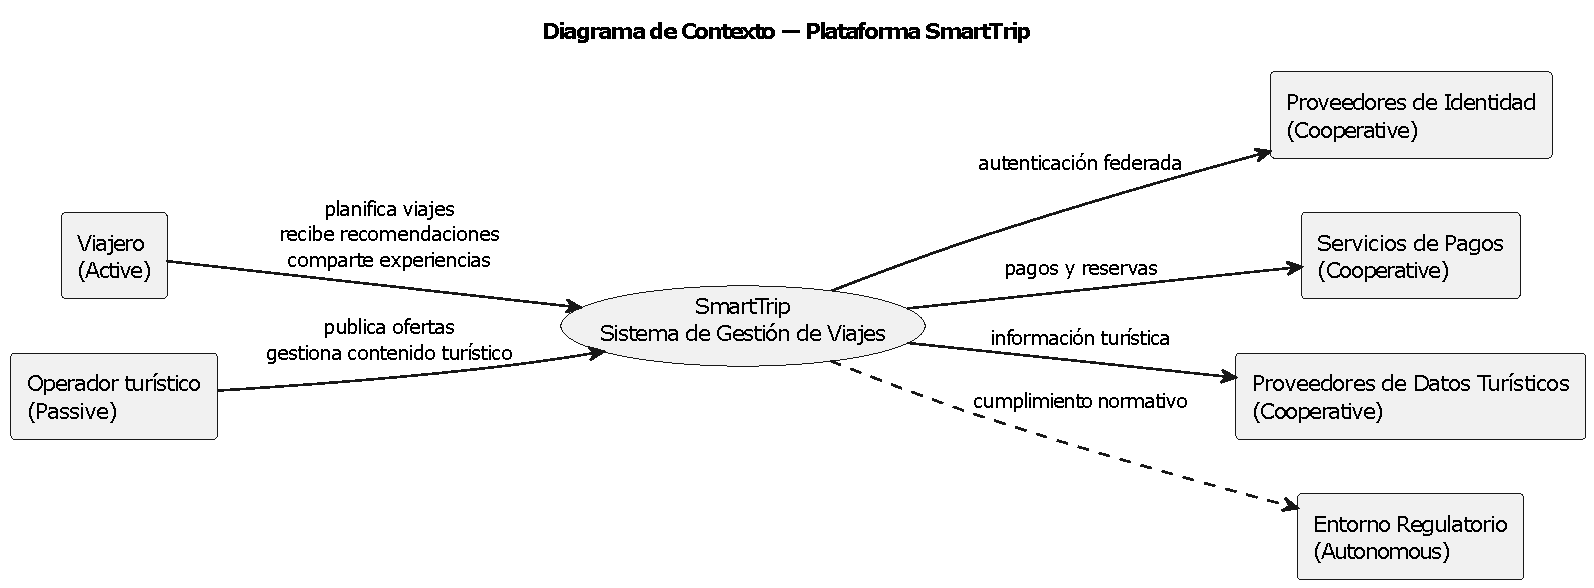
\includegraphics[width=0.9\linewidth,height=0.52\textheight,keepaspectratio]{../assets/figures/uml.context.system-context.pdf}
    \caption{Diagrama de contexto del sistema}
\end{figure}
\noindent\textit{Explicación:} La vista de contexto UML complementa C4 al explicitar actores externos y contratos de interacción relevantes para seguridad e integración.

\begin{figure}[htbp]
    \centering
    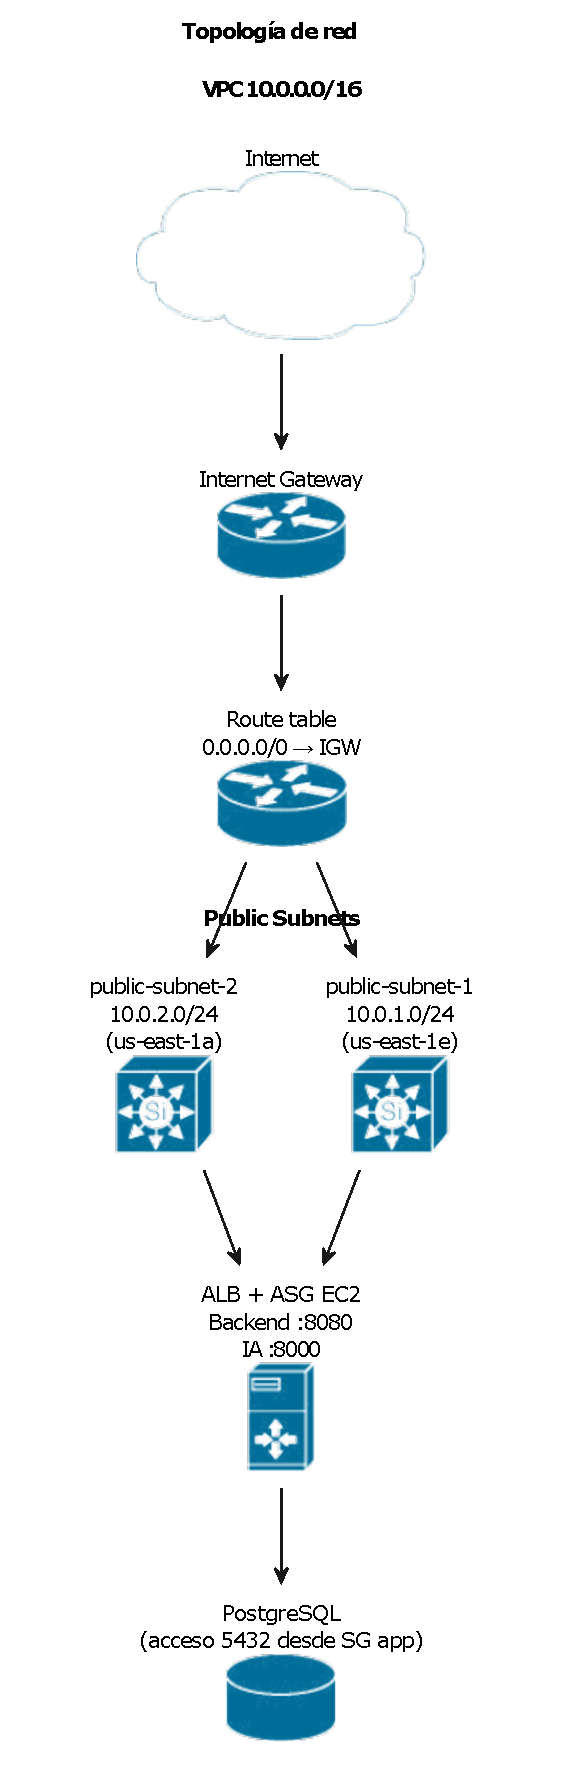
\includegraphics[width=0.88\linewidth,height=0.55\textheight,keepaspectratio]{../assets/figures/uml.deployment.network-topology.pdf}
    \caption{Topología de red en AWS}
\end{figure}
\noindent\textit{Explicación:} La topología de red muestra segmentación y rutas de tráfico, evidenciando controles de aislamiento y exposición mínima de servicios.

\begin{figure}[htbp]
    \centering
    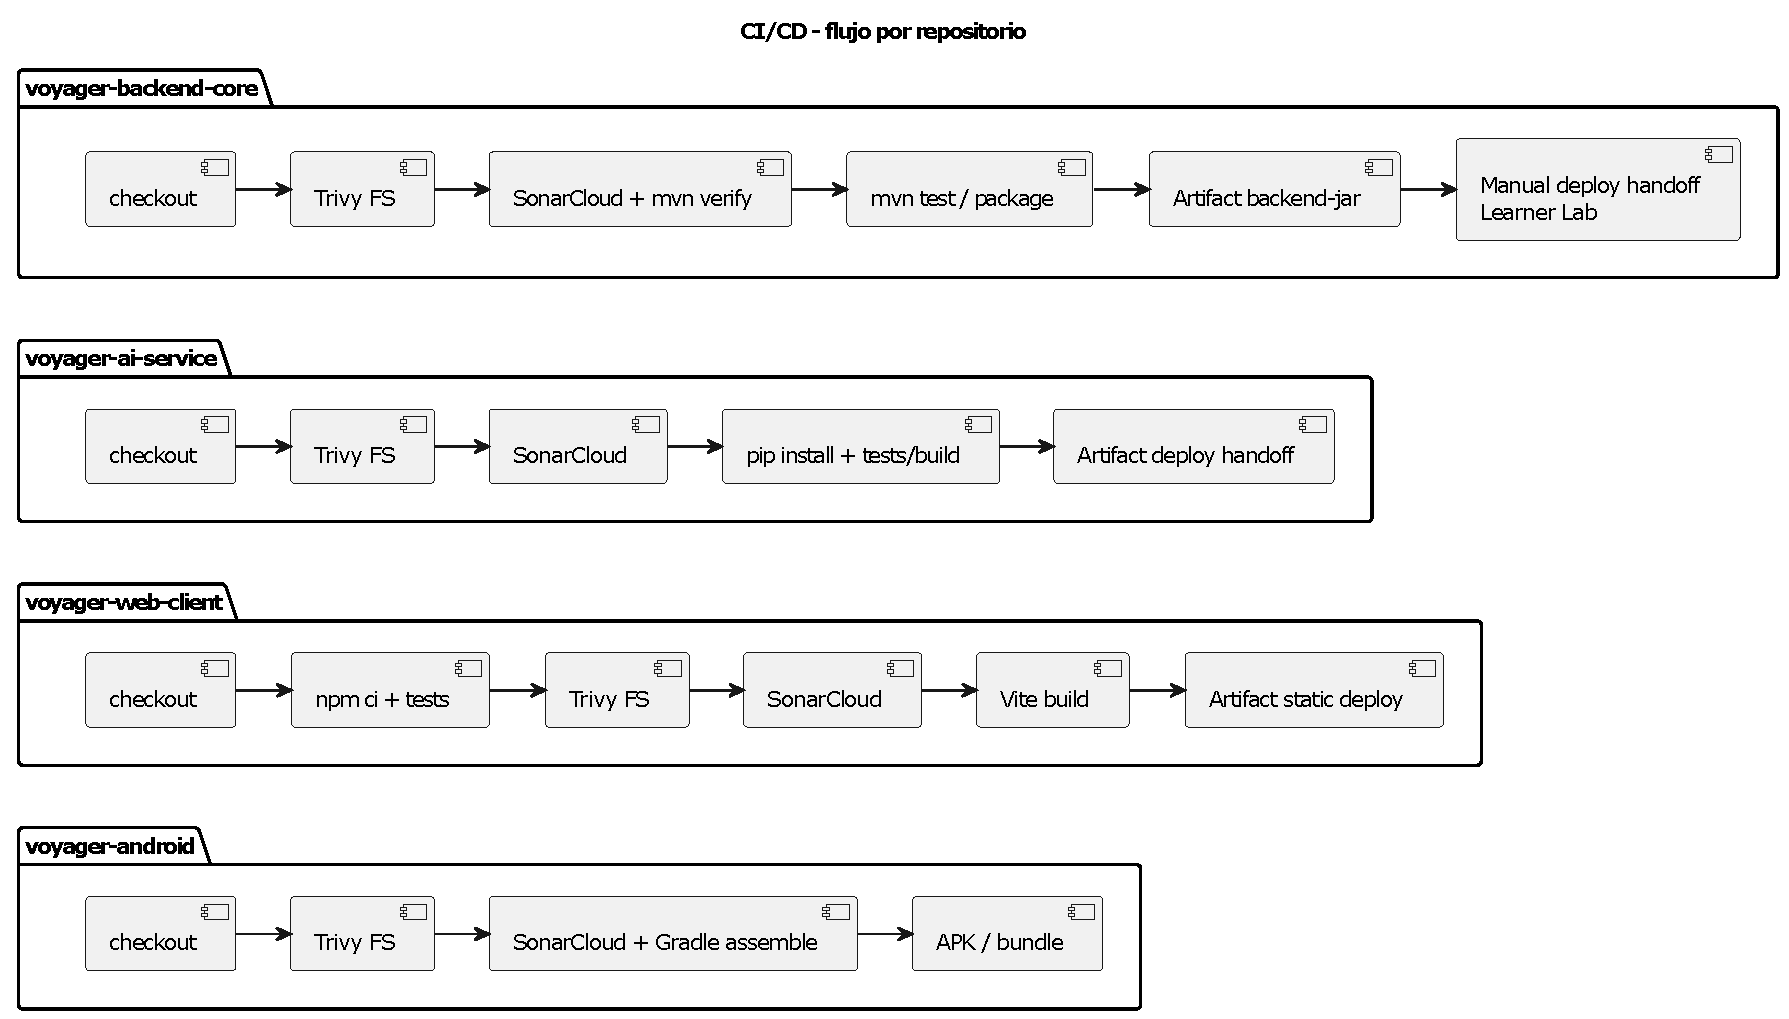
\includegraphics[width=0.9\linewidth,height=0.52\textheight,keepaspectratio]{../assets/figures/uml.deployment.cicd-pipeline.pdf}
    \caption{Pipeline de CI/CD del sistema}
\end{figure}
\noindent\textit{Explicación:} El pipeline CI/CD relaciona calidad de código, seguridad y despliegue, reduciendo riesgo de regresiones en la evolución del prototipo.

\subsection*{Síntesis crítica de hallazgos a partir de diagramas}

La revisión conjunta de C4, UML y ArchiMate muestra coherencia de alto nivel entre capacidades de negocio y componentes técnicos; sin embargo, también expone dos brechas de calidad documental que deben tratarse para evaluación académica estricta. Primero, algunos flujos conductuales UML son conceptualmente válidos pero demasiado sintéticos para sustentar pruebas de calidad sin anexar escenarios alternos y de error. Segundo, la trazabilidad entre diagramas y resultados medidos debe hacerse explícita mediante una matriz \textit{diagrama $\rightarrow$ decisión $\rightarrow$ métrica $\rightarrow$ evidencia}.

Por tanto, los diagramas se adoptan como \textbf{artefactos de diseño y verificación de consistencia}, no como evidencia empírica por sí sola. La evidencia empírica se consolida en la sección de resultados y en los indicadores operativos definidos en KPIs.

%================================================================================
\section{Atributos de Calidad del Sistema}
%================================================================================

Los atributos de calidad del sistema se han diseñado como escenarios verificables que orientan las decisiones arquitectónicas y operativas. Los siguientes diagramas detallan cada atributo de calidad con sus respectivas estrategias de implementación, presentados en formato compacto para demostrar la robustez de nuestra arquitectura.

Para fortalecer su valor argumentativo, cada escenario se interpreta con el esquema \textit{fuente-estímulo-entorno-respuesta-medida} y se vincula a una decisión técnica concreta (autoescalado, mensajería asíncrona, controles de acceso, observabilidad, IaC y seguridad en despliegue).

\begin{figure}[htbp]
    \centering
    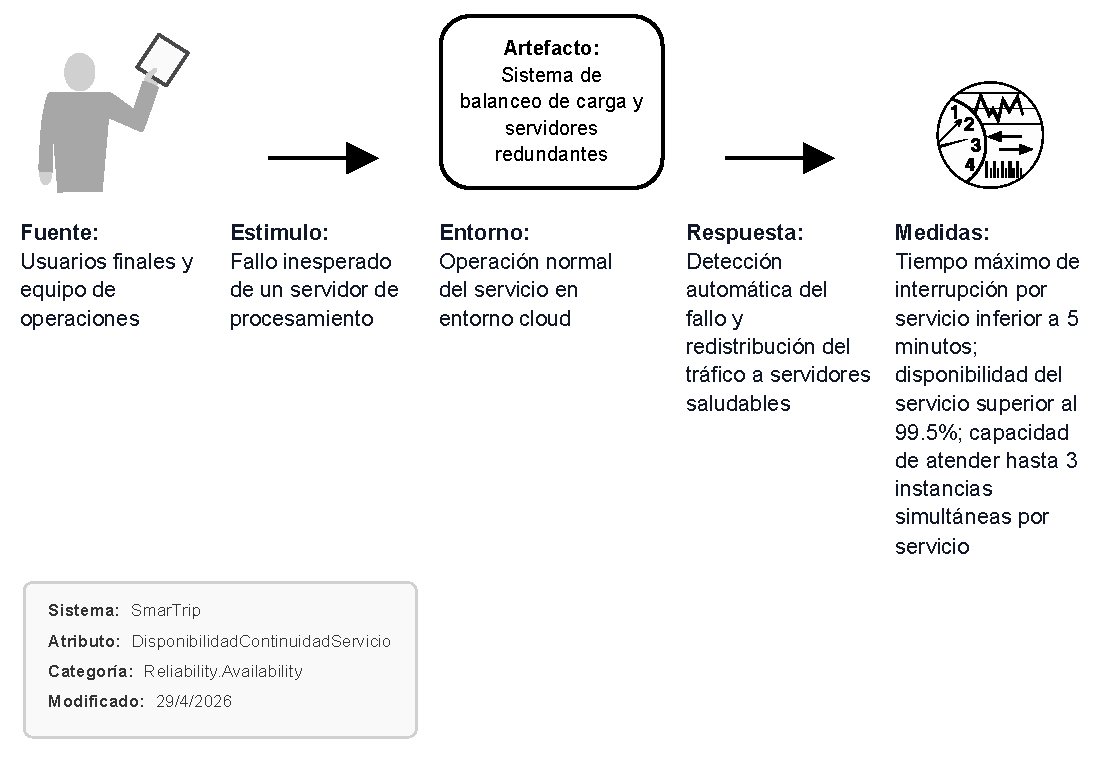
\includegraphics[width=0.88\linewidth,height=0.48\textheight,keepaspectratio]{../assets/figures/quality-attributes.SmarTrip_DisponibilidadContinuidadServicio.pdf}
    \caption{Disponibilidad y continuidad del servicio}
\end{figure}
\noindent\textit{Explicación:} Este escenario define respuesta ante fallos de cómputo y sustenta decisiones de redundancia y balanceo para continuidad operativa.

\begin{figure}[htbp]
    \centering
    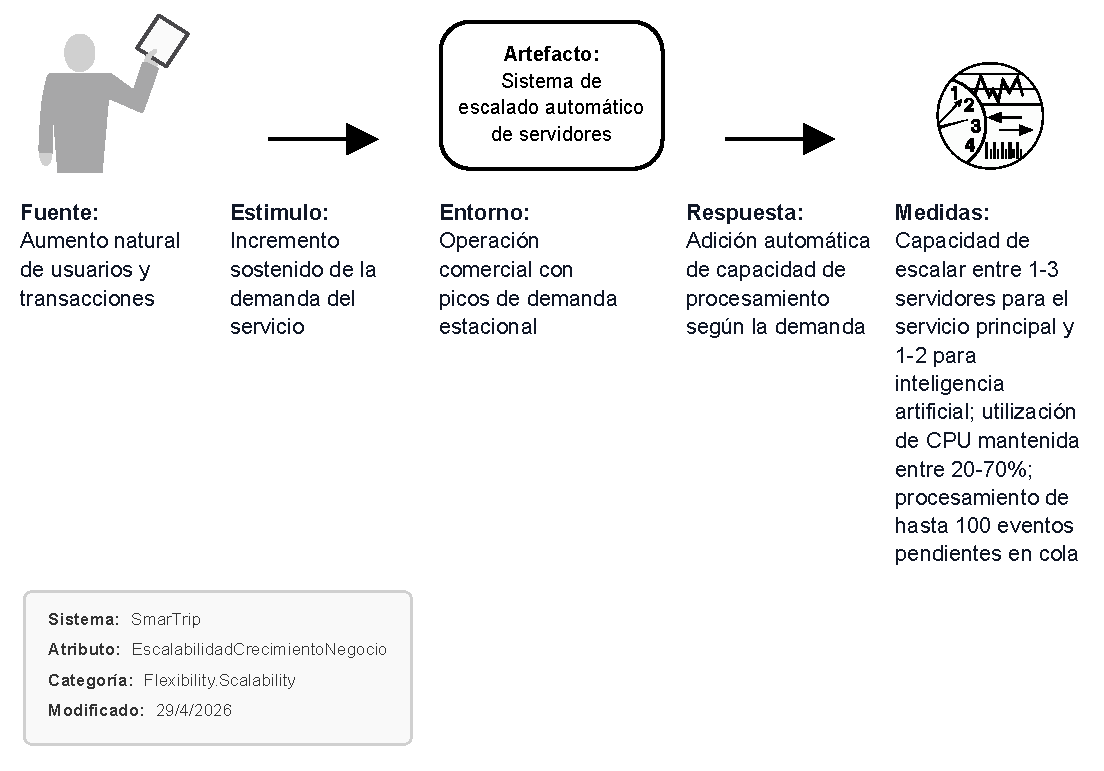
\includegraphics[width=0.88\linewidth,height=0.48\textheight,keepaspectratio]{../assets/figures/quality-attributes.SmarTrip_EscalabilidadCrecimientoNegocio.pdf}
    \caption{Escalabilidad y crecimiento del negocio}
\end{figure}
\noindent\textit{Explicación:} La vista establece cómo la plataforma incrementa capacidad ante demanda creciente sin degradar de forma abrupta la experiencia.

\begin{figure}[htbp]
    \centering
    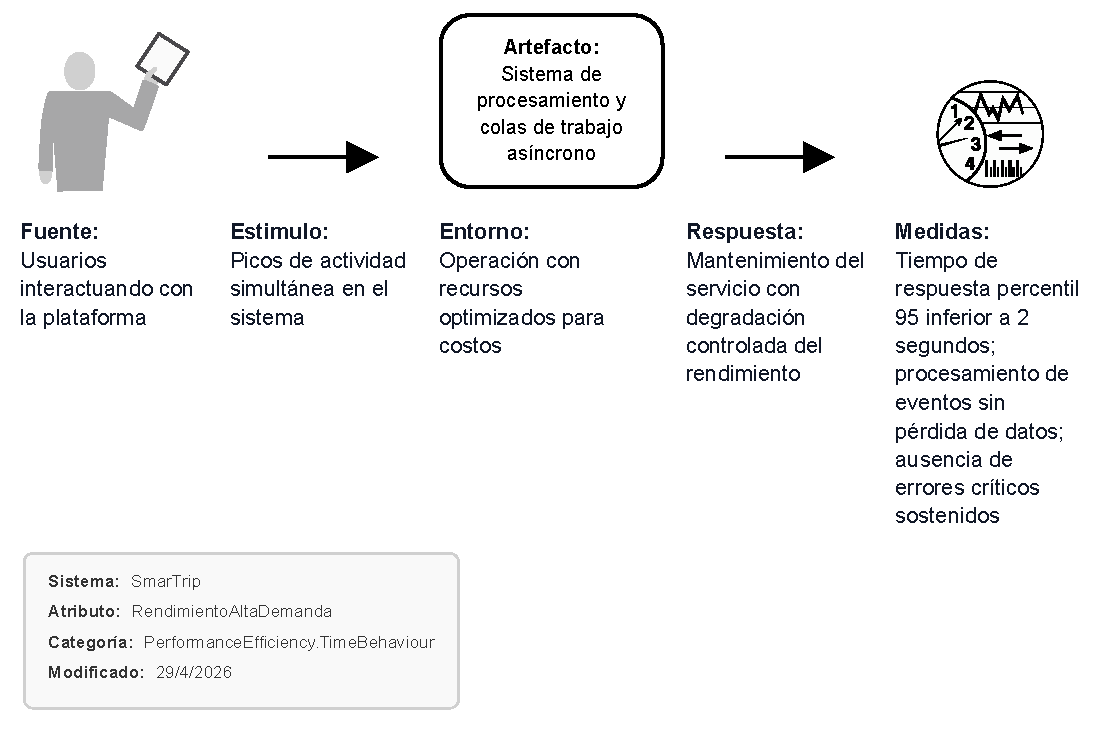
\includegraphics[width=0.88\linewidth,height=0.48\textheight,keepaspectratio]{../assets/figures/quality-attributes.SmarTrip_RendimientoAltaDemanda.pdf}
    \caption{Rendimiento bajo alta demanda}
\end{figure}
\noindent\textit{Explicación:} El atributo de rendimiento fija umbrales de latencia y error para escenarios de pico, conectando operación con objetivos de servicio.

\begin{figure}[htbp]
    \centering
    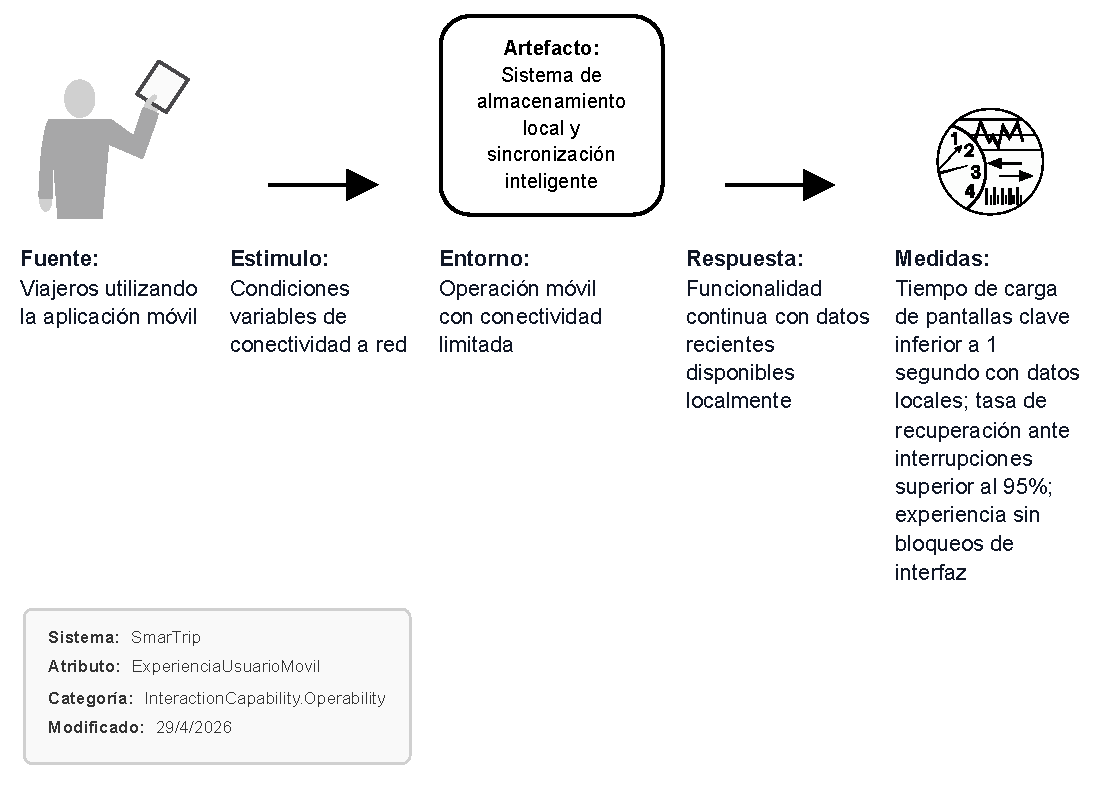
\includegraphics[width=0.88\linewidth,height=0.48\textheight,keepaspectratio]{../assets/figures/quality-attributes.SmarTrip_ExperienciaUsuarioMovil.pdf}
    \caption{Experiencia de usuario móvil}
\end{figure}
\noindent\textit{Explicación:} Esta especificación prioriza continuidad funcional en movilidad y conectividad limitada, crítica para adopción en campo.

\begin{figure}[htbp]
    \centering
    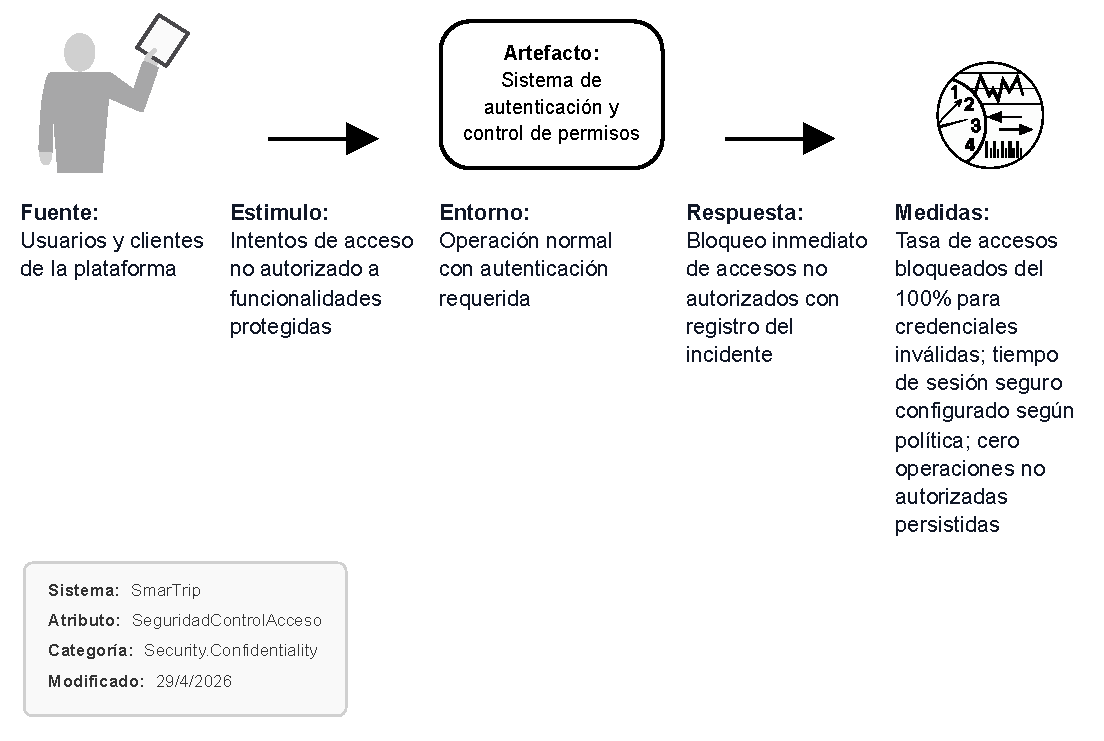
\includegraphics[width=0.88\linewidth,height=0.48\textheight,keepaspectratio]{../assets/figures/quality-attributes.SmarTrip_SeguridadControlAcceso.pdf}
    \caption{Seguridad y control de acceso}
\end{figure}
\noindent\textit{Explicación:} El diagrama formaliza autenticación y autorización como controles preventivos para evitar operaciones no permitidas.

\begin{figure}[htbp]
    \centering
    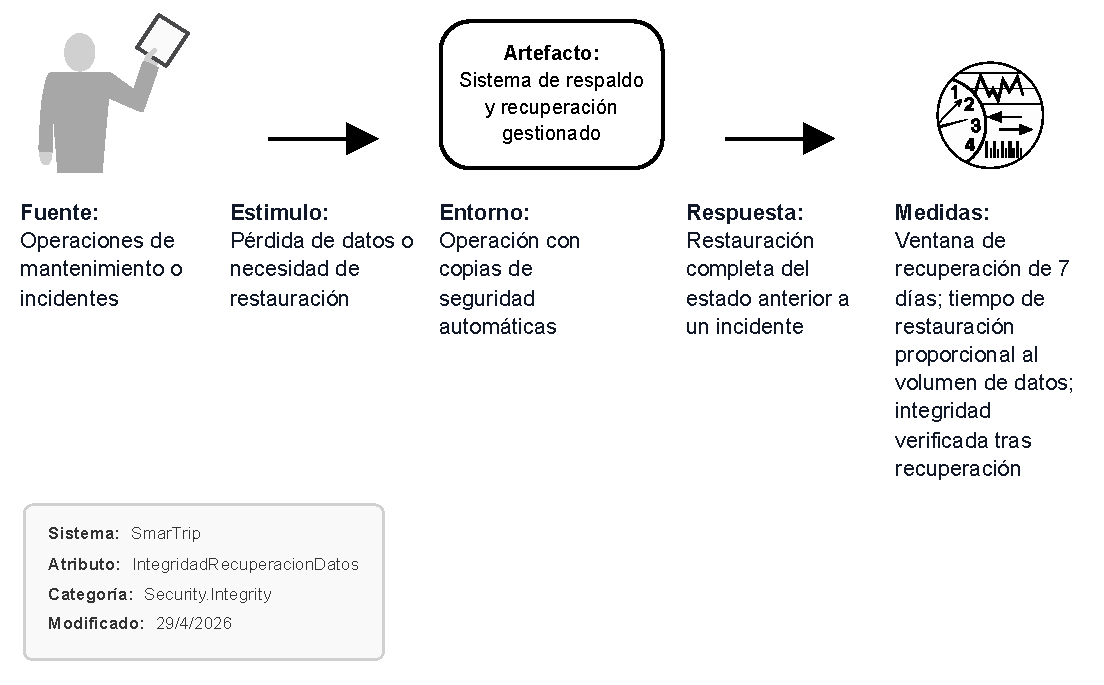
\includegraphics[width=0.88\linewidth,height=0.48\textheight,keepaspectratio]{../assets/figures/quality-attributes.SmarTrip_IntegridadRecuperacionDatos.pdf}
    \caption{Integridad y recuperación de datos}
\end{figure}
\noindent\textit{Explicación:} Esta vista vincula política de respaldo y restauración con objetivos de recuperación y preservación de consistencia de datos.

\begin{figure}[htbp]
    \centering
    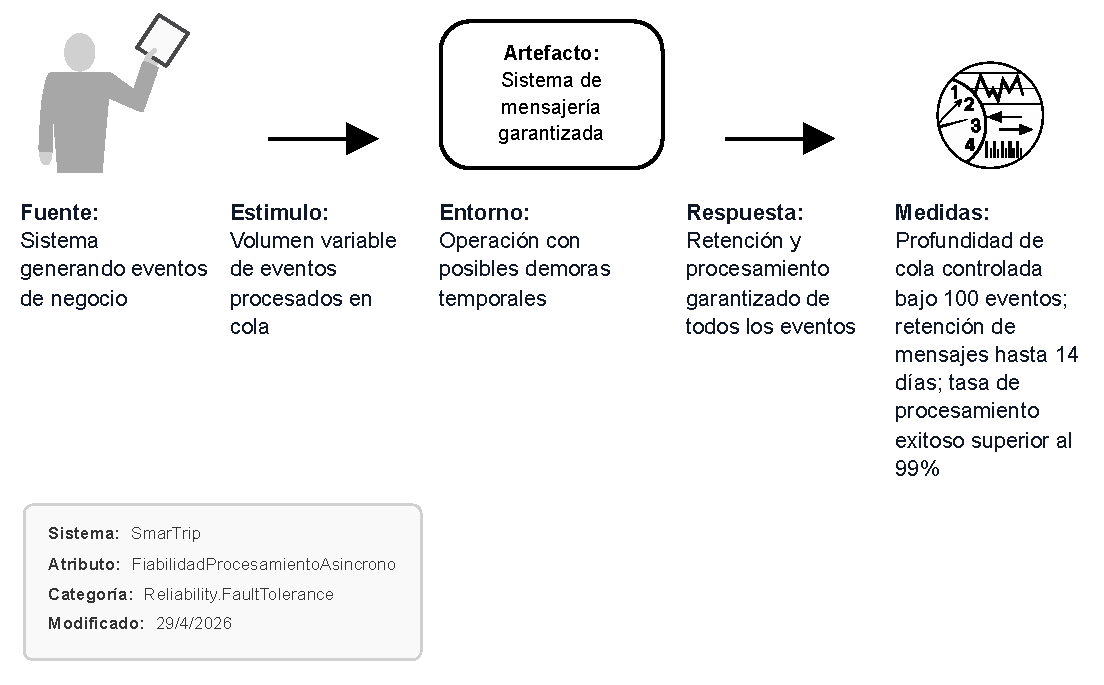
\includegraphics[width=0.88\linewidth,height=0.48\textheight,keepaspectratio]{../assets/figures/quality-attributes.SmarTrip_FiabilidadProcesamientoAsincrono.pdf}
    \caption{Fiabilidad del procesamiento asíncrono}
\end{figure}
\noindent\textit{Explicación:} El escenario valida robustez de mensajería ante variabilidad de carga y evita pérdida de eventos de negocio.

\begin{figure}[htbp]
    \centering
    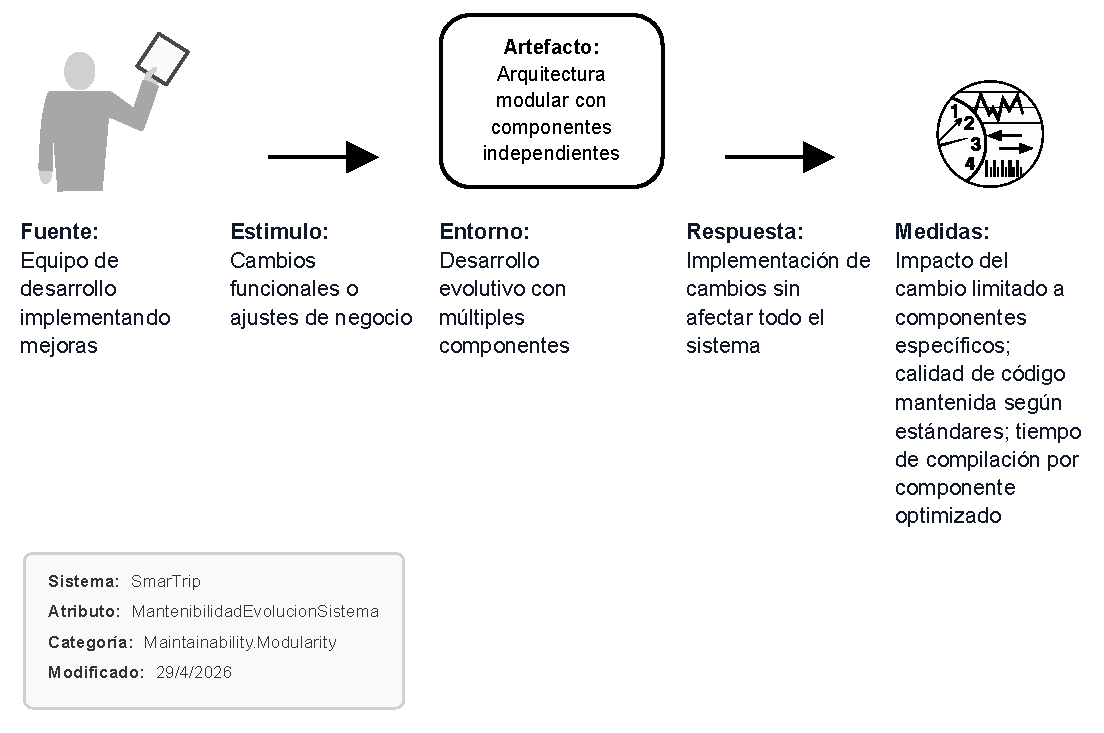
\includegraphics[width=0.88\linewidth,height=0.48\textheight,keepaspectratio]{../assets/figures/quality-attributes.SmarTrip_MantenibilidadEvolucionSistema.pdf}
    \caption{Mantenibilidad y evolución del sistema}
\end{figure}
\noindent\textit{Explicación:} Esta especificación respalda modularidad y cambios localizados, reduciendo impacto transversal durante evolución funcional.

\begin{figure}[htbp]
    \centering
    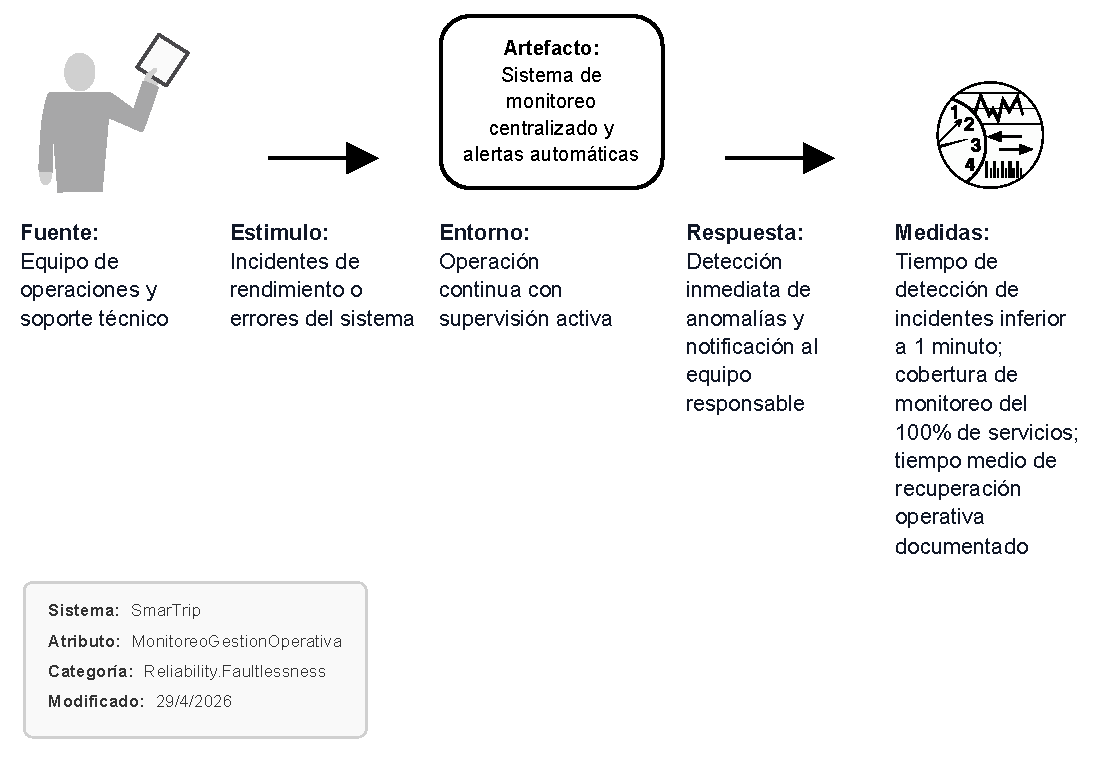
\includegraphics[width=0.88\linewidth,height=0.48\textheight,keepaspectratio]{../assets/figures/quality-attributes.SmarTrip_MonitoreoGestionOperativa.pdf}
    \caption{Monitoreo y gestión operativa}
\end{figure}
\noindent\textit{Explicación:} El atributo de monitoreo define detección temprana de incidentes y tiempos de respuesta para operación continua.

\begin{figure}[htbp]
    \centering
    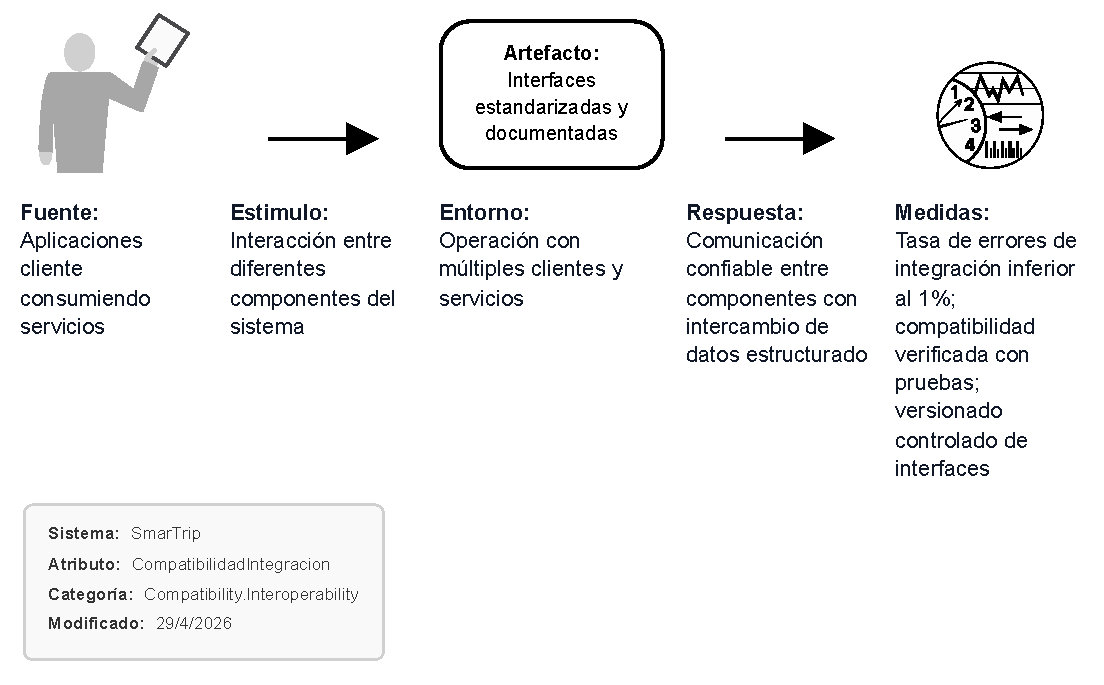
\includegraphics[width=0.88\linewidth,height=0.48\textheight,keepaspectratio]{../assets/figures/quality-attributes.SmarTrip_CompatibilidadIntegracion.pdf}
    \caption{Compatibilidad e integración}
\end{figure}
\noindent\textit{Explicación:} Esta vista enfatiza contratos estables e interoperabilidad entre módulos y servicios externos en evolución continua.

\begin{figure}[htbp]
    \centering
    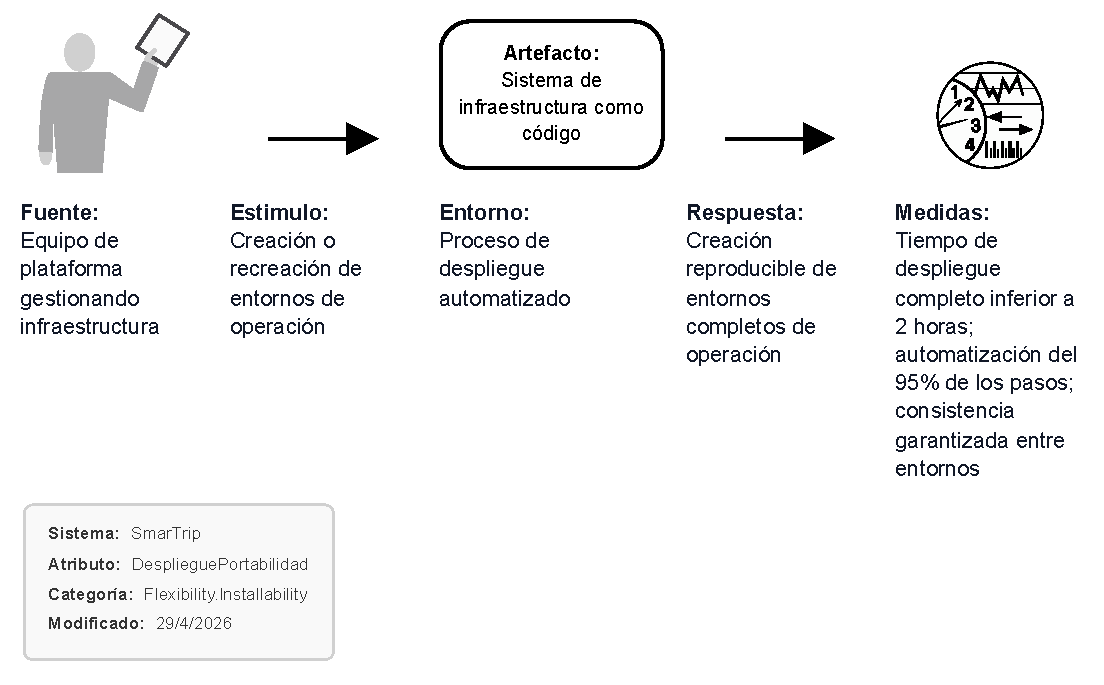
\includegraphics[width=0.88\linewidth,height=0.48\textheight,keepaspectratio]{../assets/figures/quality-attributes.SmarTrip_DesplieguePortabilidad.pdf}
    \caption{Despliegue y portabilidad}
\end{figure}
\noindent\textit{Explicación:} El escenario relaciona IaC y reproducibilidad de entornos para disminuir variabilidad entre desarrollo, prueba y operación.

\begin{figure}[htbp]
    \centering
    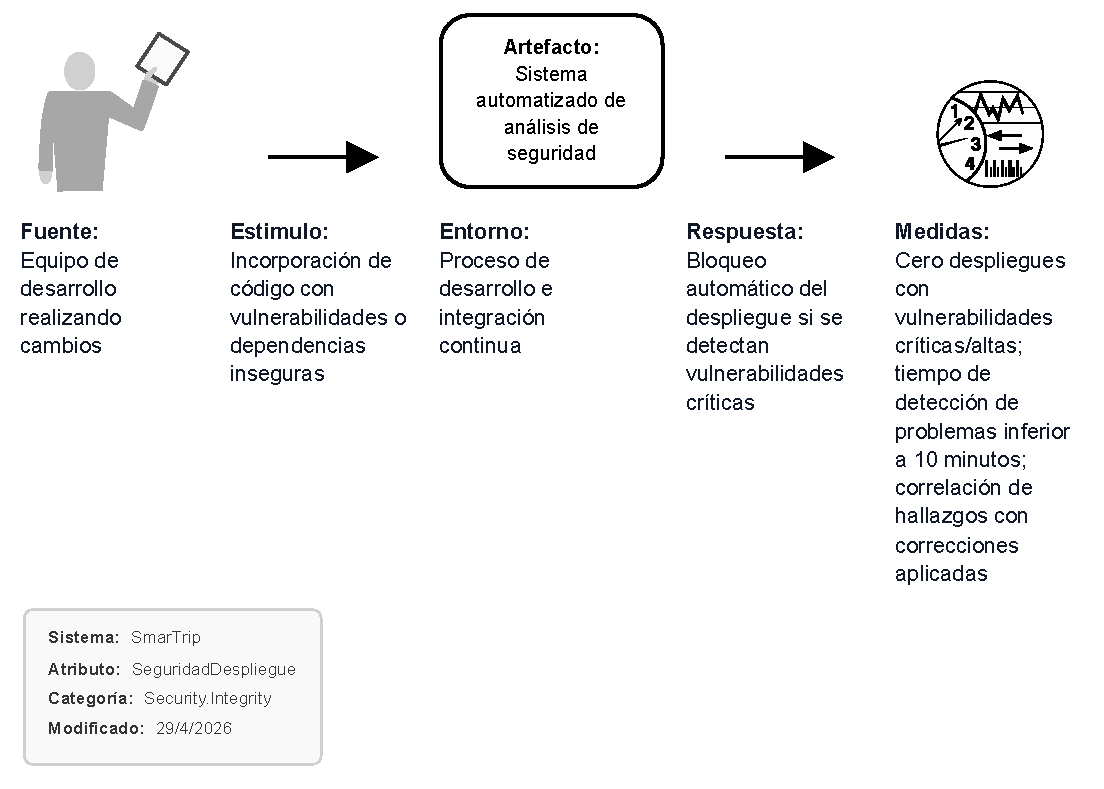
\includegraphics[width=0.88\linewidth,height=0.48\textheight,keepaspectratio]{../assets/figures/quality-attributes.SmarTrip_SeguridadDespliegue.pdf}
    \caption{Seguridad en el despliegue}
\end{figure}
\noindent\textit{Explicación:} La seguridad de despliegue asegura que vulnerabilidades críticas bloqueen promoción de artefactos a entornos superiores.

\begin{figure}[htbp]
    \centering
    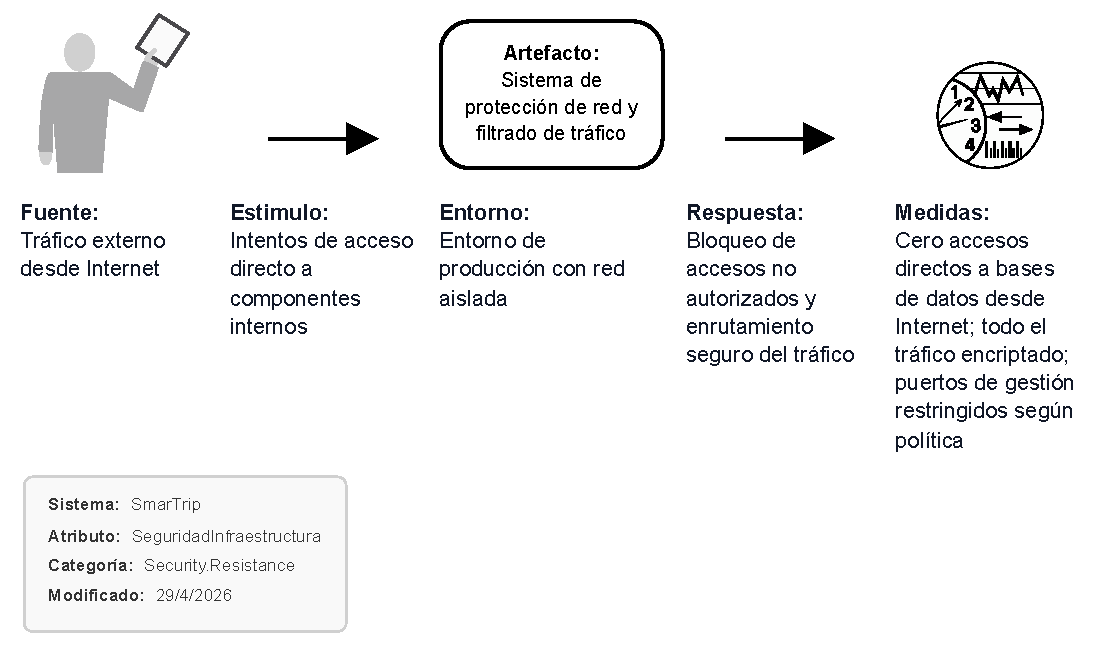
\includegraphics[width=0.88\linewidth,height=0.48\textheight,keepaspectratio]{../assets/figures/quality-attributes.SmarTrip_SeguridadInfraestructura.pdf}
    \caption{Seguridad de la infraestructura}
\end{figure}
\noindent\textit{Explicación:} Este atributo valida endurecimiento de red e infraestructura para minimizar superficie de ataque en operación cloud.

\subsection*{Interpretación integrada de atributos de calidad}

Los atributos de \textbf{disponibilidad, escalabilidad y rendimiento} convergen en una misma decisión arquitectónica: desacoplar procesamiento transaccional e IA y absorber variabilidad con colas y autoescalado. Los atributos de \textbf{seguridad e integridad} muestran controles de acceso, segmentación de red y prácticas de despliegue seguro, pero requieren respaldo continuo con evidencia operacional (logs de auditoría, reportes de vulnerabilidades y pruebas de restauración). Finalmente, los atributos de \textbf{mantenibilidad, compatibilidad y portabilidad} justifican la modularidad y la infraestructura reproducible, condicionadas a disciplina de versionado y pruebas de regresión entre interfaces.

Como mejora metodológica, se define que cada atributo debe reportarse periódicamente con evidencia cuantitativa mínima: disponibilidad mensual, p95 de latencia, tasa de errores de integración, incidentes de seguridad bloqueados y tiempo de restauración.

\newpage

%================================================================================
\section{Cronograma y Presupuesto de Montaje Empresarial}
%================================================================================

\subsection{Cronograma de Implementación}

El cronograma de montaje empresarial se estructura en fases secuenciales con hitos claros para garantizar una transformación digital ordenada y medible:

\begin{figure}[htbp]
    \centering
    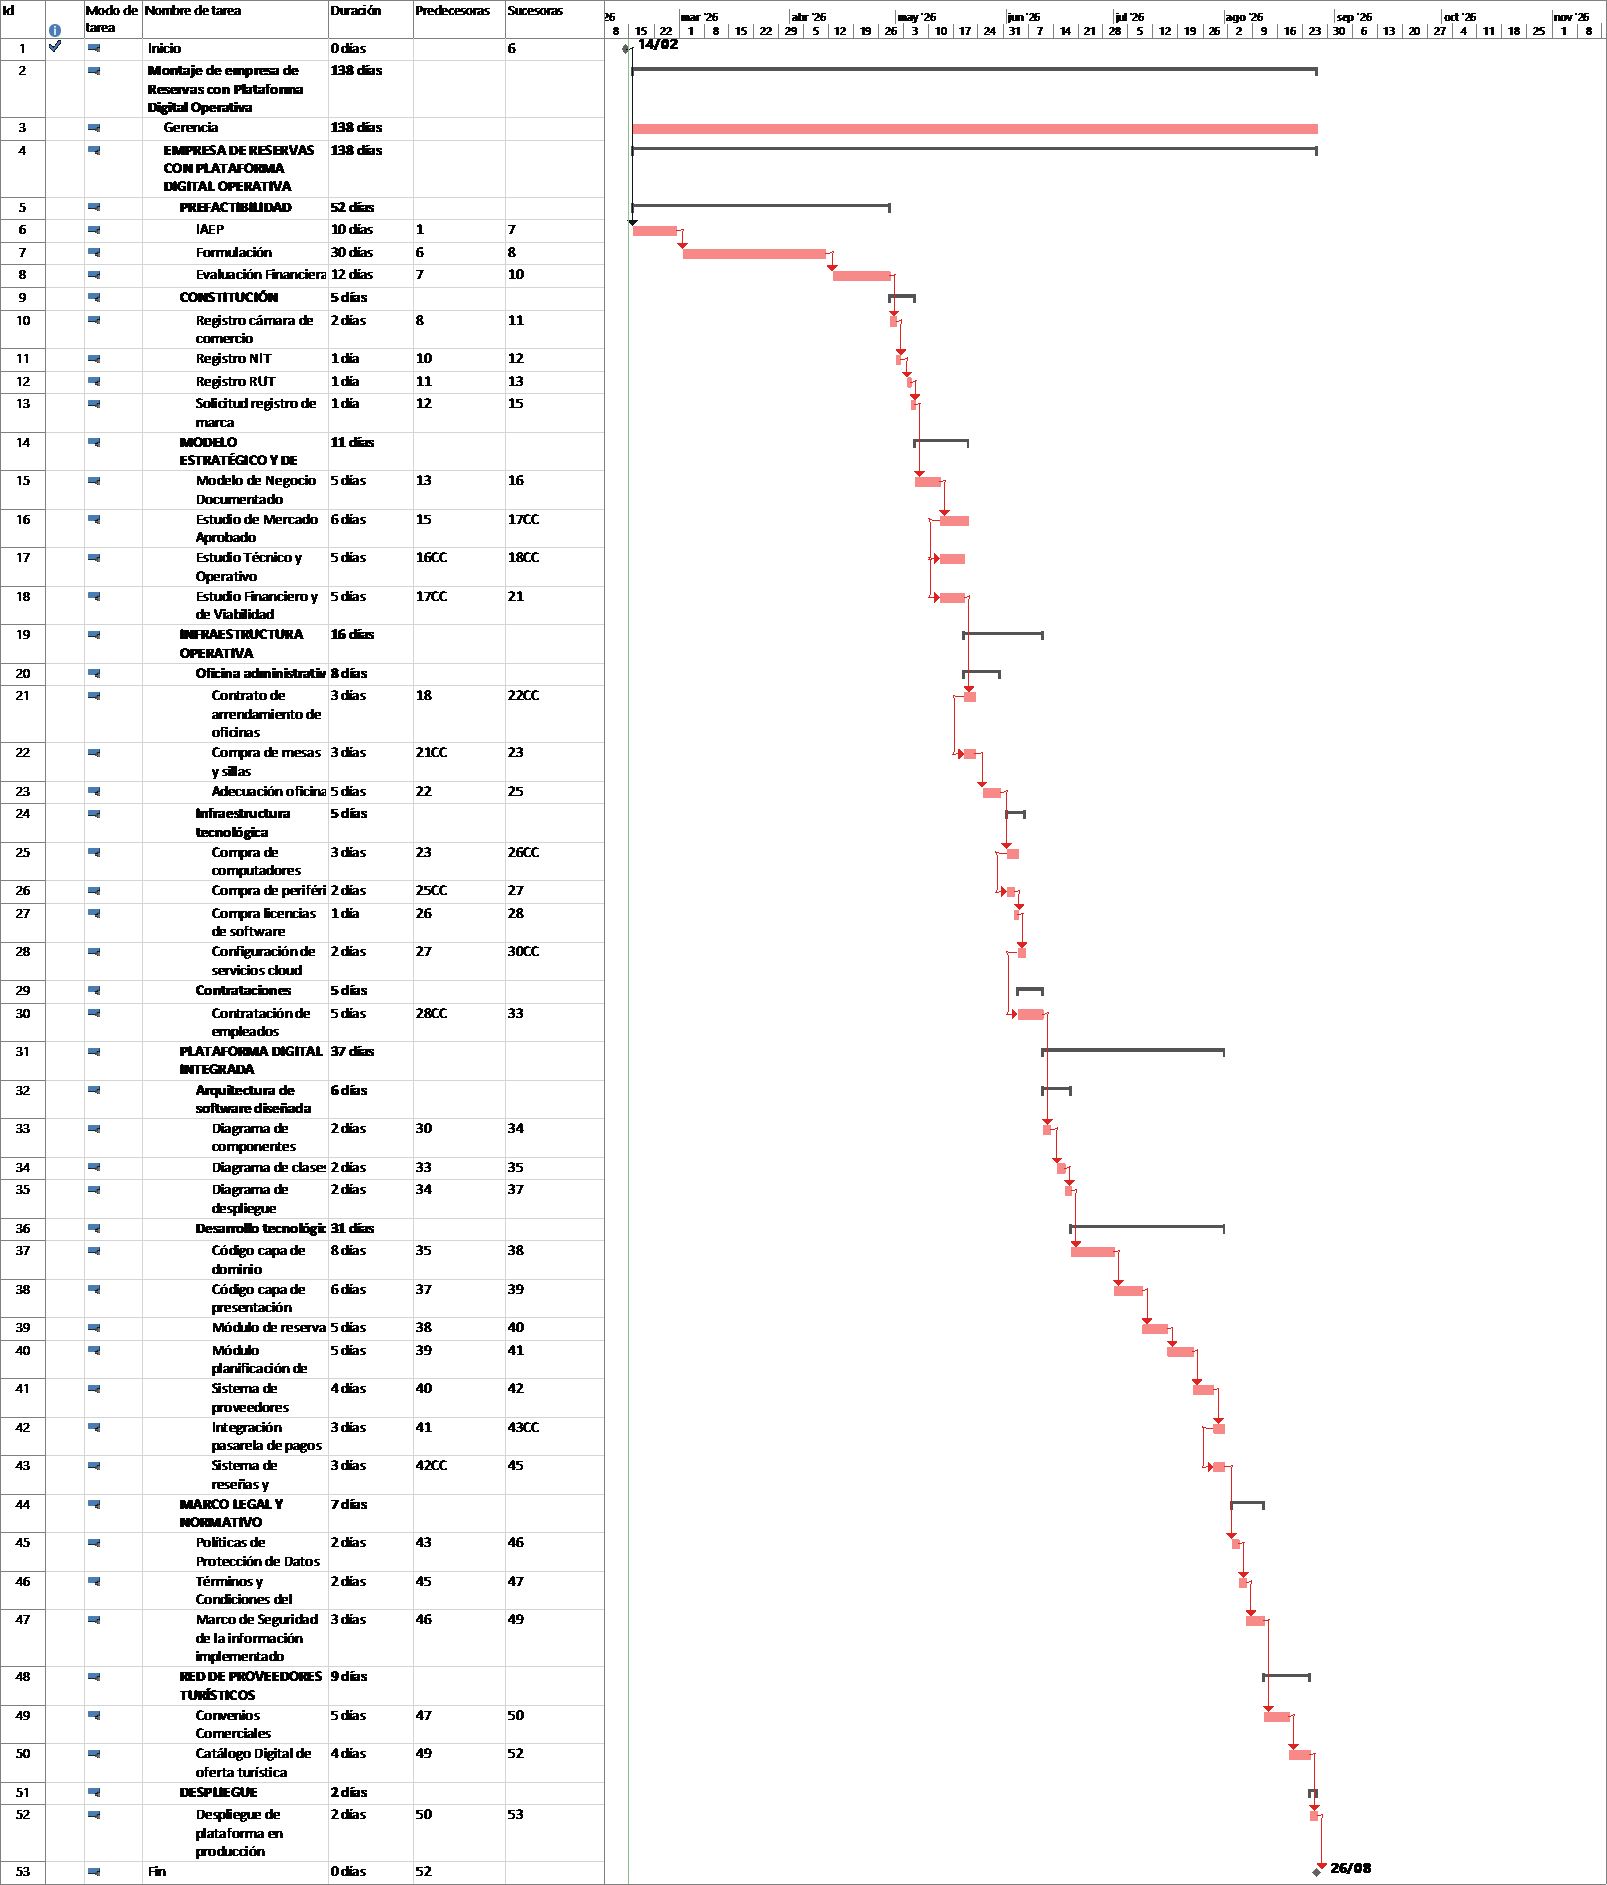
\includegraphics[width=0.92\linewidth,height=0.72\textheight,keepaspectratio]{../assets/img/epro.Planteamiento_Proyecto_img-007.png}
    \caption{Cronograma de implementación del proyecto}
\end{figure}

\subsection{Presupuesto de Inversión}

El presupuesto detallado contempla inversiones en infraestructura, desarrollo, marketing y operación:

\begin{figure}[htbp]
    \centering
    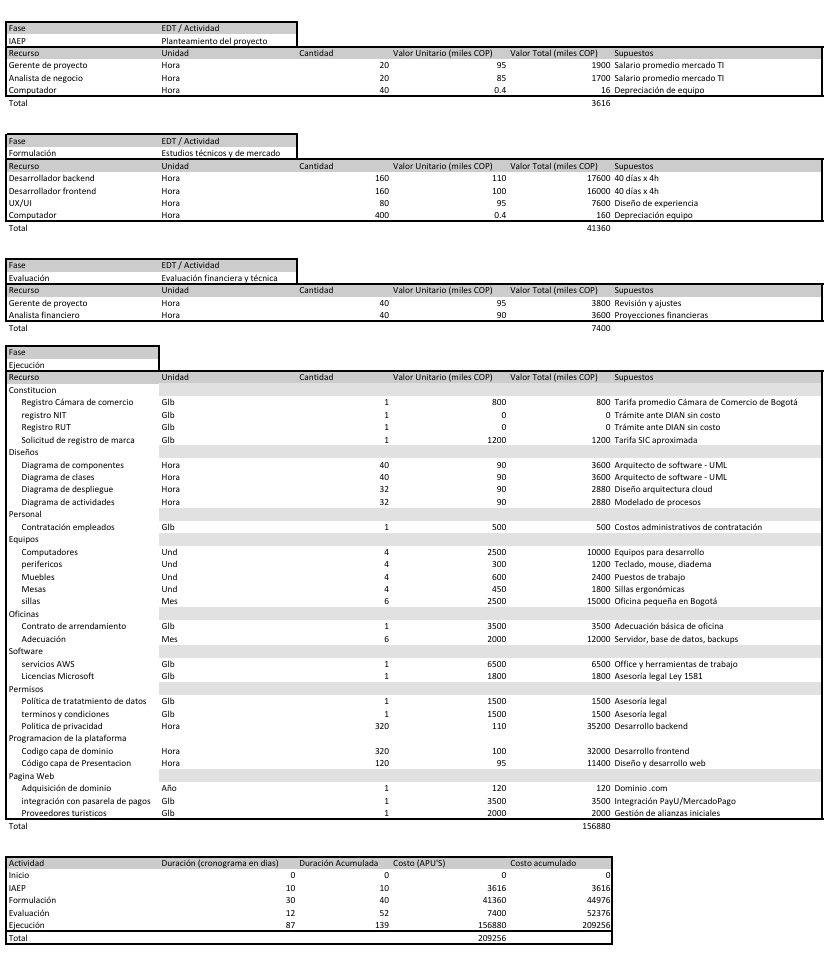
\includegraphics[width=0.92\linewidth,height=0.72\textheight,keepaspectratio]{../assets/img/epro.Planteamiento_Proyecto_img-009.png}
    \caption{Presupuesto de montaje empresarial}
\end{figure}

\subsection{Análisis Financiero Estratégico}

El análisis financiero estratégico fundamenta la viabilidad económica de la plataforma de transformación digital turística, utilizando como fuente de verdad el memo de inversión evaluado. Esta evaluación comprehensiva demuestra que el modelo de negocio es viable con disciplina financiera y ejecución estratégica, transformando una oportunidad de mercado en un negocio invertible con control sobre márgenes y escalabilidad.

\paragraph{Inversión Inicial y Asignación Estratégica de Capital}

La inversión inicial requerida asciende a \$218.087.168 COP, distribuida estratégicamente para construir capacidades tecnológicas diferenciadoras. El 84\% de esta inversión (\$183.125.667 COP) se destina al desarrollo tecnológico MVP, abarcando desarrollo full-stack (React, Android, Spring Boot), infraestructura cloud base e integración de APIs y sistemas de pago. Esta asignación prioritaria en tecnología garantiza una base sólida para escalamiento y diferenciación funcional en el mercado turístico colombiano.

\begin{figure}[htbp]
    \centering
    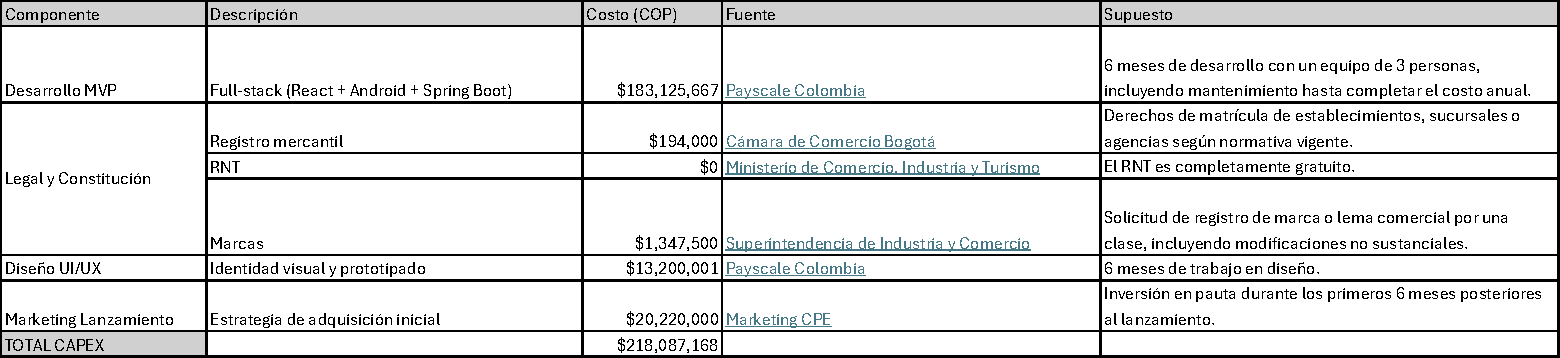
\includegraphics[width=\textwidth]{../assets/figures/finance.capex.pdf}
    \caption{Inversión Inicial (CAPEX) - Distribución estratégica por componentes}
\end{figure}

El diseño UI/UX representa el 6.1\% (\$13.200.001 COP) y es fundamental para la experiencia del usuario, incluyendo identidad visual, prototipado y testing de experiencia responsive. El marketing de lanzamiento constituye el 9.3\% (\$20.220.000 COP) para estrategias de adquisición inicial y activación de primeros usuarios. Los aspectos legales y corporativos, aunque solo el 0.6\% (\$1.347.500 COP), son críticos para la constitución de sociedad, registro mercantil, RNT y propiedad intelectual.

\paragraph{Arquitectura Cloud e Infraestructura Escalable}

La infraestructura tecnológica se diseña bajo una arquitectura de alta disponibilidad y escalabilidad en AWS, garantizando continuidad del negocio y capacidad de crecimiento sin degradación del servicio. La arquitectura Multi-AZ con disponibilidad del 99.99\% representa una ventaja competitiva significativa frente a competidores con arquitecturas menos robustas.

\begin{figure}[htbp]
    \centering
    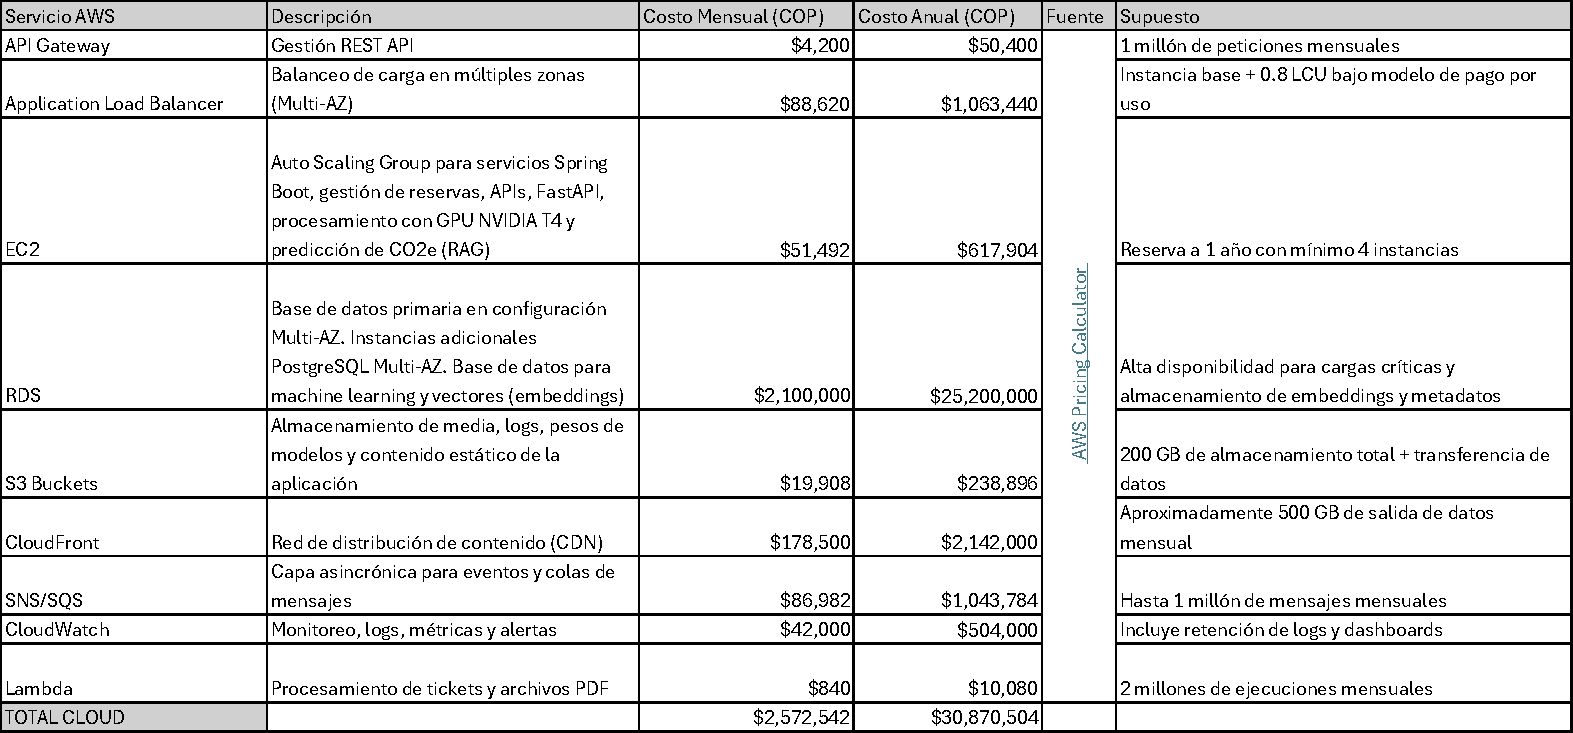
\includegraphics[width=\textwidth]{../assets/figures/finance.cloud.pdf}
    \caption{Arquitectura de Infraestructura Cloud (AWS) - Diseño redundante y escalable}
\end{figure}

Los componentes principales incluyen API Gateway para gestión de endpoints, Application Load Balancer para distribución de carga, CloudFront CDN para optimización de contenido, instancias EC2 para procesamiento principal, RDS Multi-AZ para bases de datos redundantes, S3 Buckets para almacenamiento escalable, SNS/SQS para mensajería asíncrona, CloudWatch para monitoreo y Lambda para procesamiento serverless.

\paragraph{Ventaja Estratégica en Inteligencia Artificial}

La capa de inteligencia artificial representa un diferenciador fundamental con una arquitectura optimizada para controlar costos variables y maximizar valor entregado. La implementación utiliza vLLM para inferencia local en EC2 AI, eliminando costos por token externos y permitiendo control directo sobre rendimiento y escalabilidad.

\begin{figure}[htbp]
    \centering
    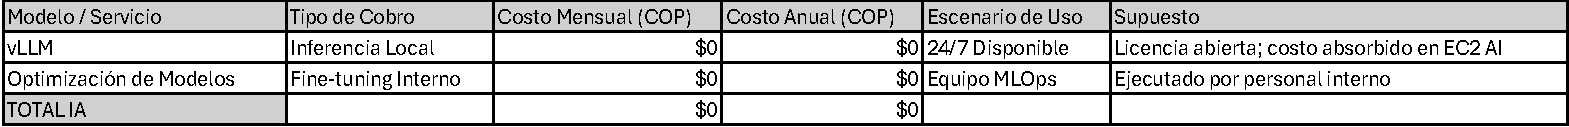
\includegraphics[width=\textwidth]{../assets/figures/finance.ai.pdf}
    \caption{Estructura de Costos de Inteligencia Artificial - Infraestructura optimizada vLLM}
\end{figure}

La capacidad GPU está diseñada para 1,500,000 requests/mes por bloque con un costo marginal de \$1.40 por request y escalabilidad automática según demanda. Esta decisión de auto-hospedar modelos de IA elimina exposición a costos variables impredecibles y protege márgenes a medida que escala el uso, permitiendo ofrecer funcionalidades avanzadas sin comprometer rentabilidad.

\paragraph{Estructura de Costos Operativos y Eficiencia}

Los costos operativos mensuales consolidados ascienden a \$29.577.542 COP (\$354.930.504 COP/año), representando una estructura eficiente para sostener una plataforma tecnológica compleja con capacidad de crecimiento. El modelo 100\% remoto reduce costos fijos en 30\% comparado con modelos tradicionales de oficina.

\begin{figure}[htbp]
    \centering
    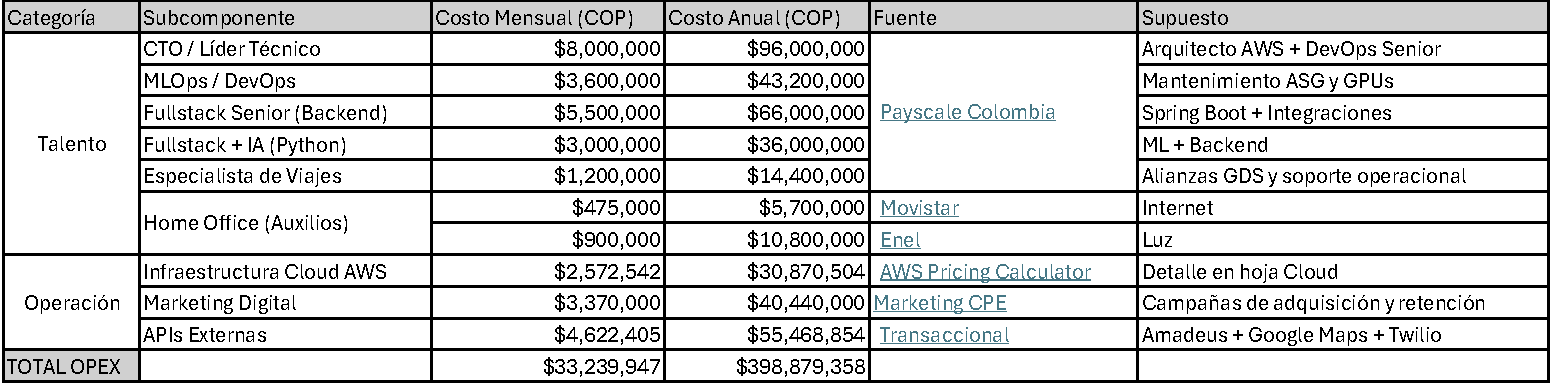
\includegraphics[width=\textwidth]{../assets/figures/finance.opex.pdf}
    \caption{Costos Operativos Mensuales - Estructura de talento humano especializado}
\end{figure}

El equipo base está compuesto por roles especializados: CTO/Líder Técnico (\$8.000.000 COP/mes), MLOps/DevOps (\$6.600.000 COP/mes), Fullstack Senior (\$7.100.000 COP/mes), Fullstack+IA (\$12.300.000 COP/mes) y Especialista Viajes (\$2.600.000 COP/mes). Los costos operativos adicionales incluyen infraestructura cloud + GPU base (\$2.602.542 COP/mes), marketing base (\$1.900.000 COP/mes) y APIs fijas integradas (\$2.400.000 COP/mes).

\paragraph{Modelo de Monetización Híbrido Diversificado}

El modelo de monetización adopta un enfoque híbrido que maximiza valor capturado a través de múltiples fuentes de ingresos, diversificando riesgos y optimizando rentabilidad por segmento. Este modelo está diseñado para capturar valor a través de comisiones transaccionales, suscripciones premium y monetización de IA.

\begin{figure}[htbp]
    \centering
    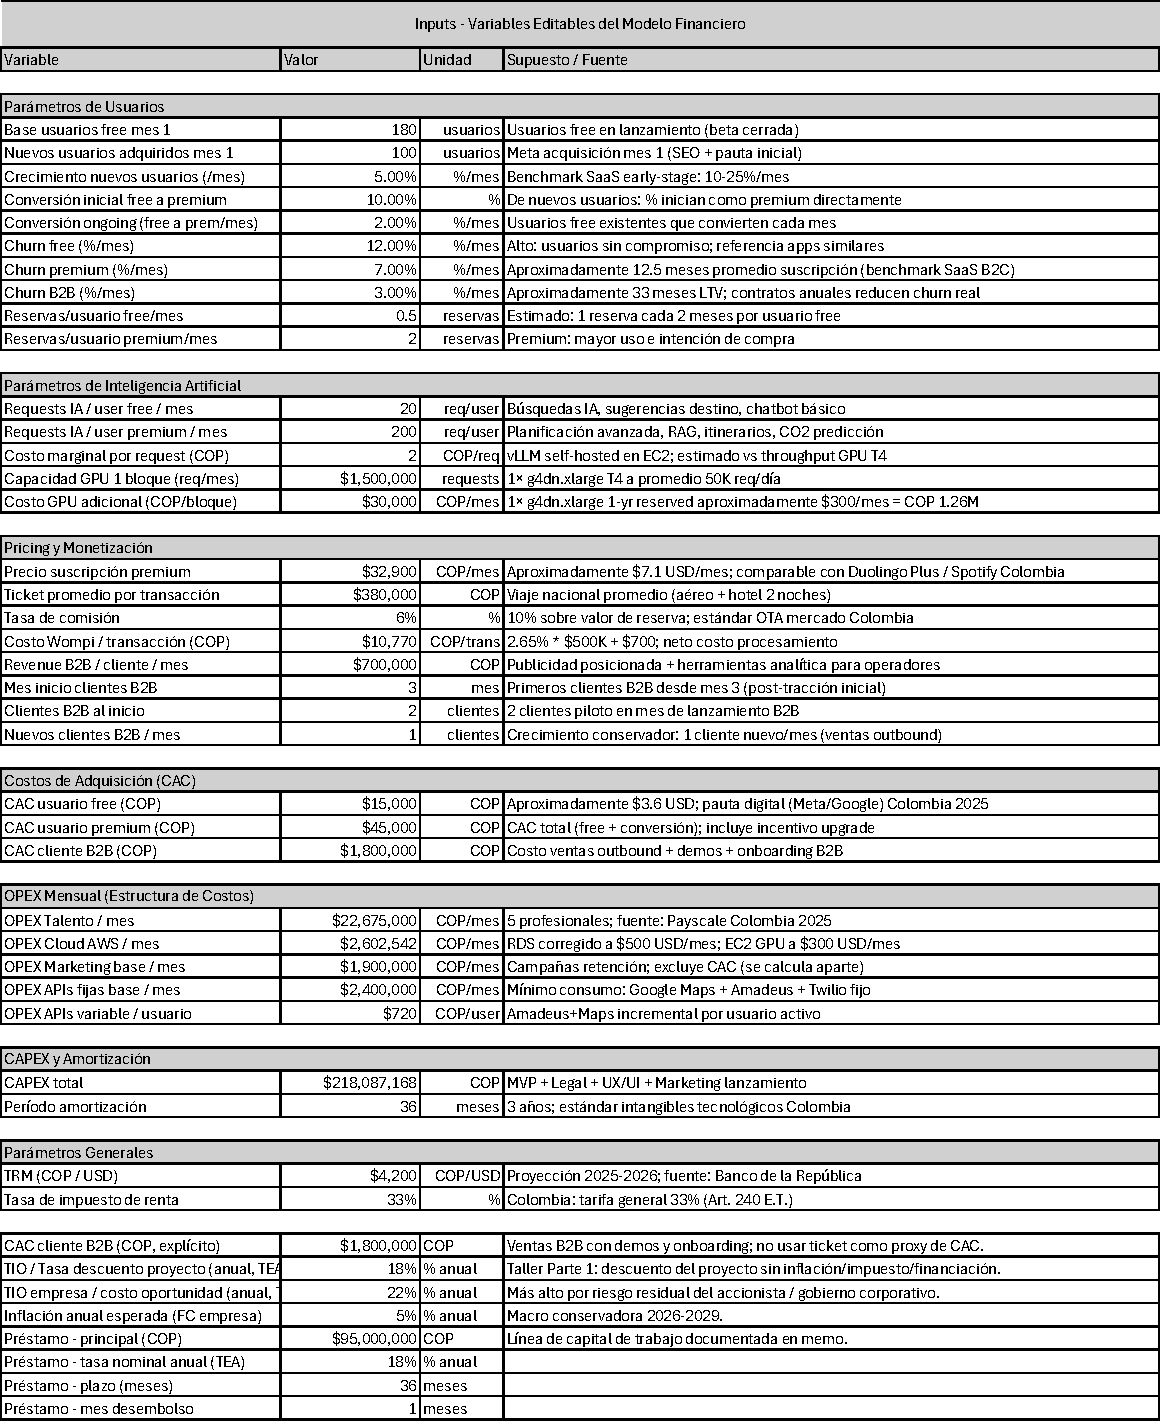
\includegraphics[width=\textwidth]{../assets/figures/finance.inputs.pdf}
    \caption{Variables y Parámetros del Modelo Financiero - Configuración estratégica}
\end{figure}

Las fuentes principales incluyen: (1) Comisiones por transacción con 5.5\% sobre reservas y 5\% sobre servicios complementarios; (2) Suscripciones premium con B2C Premium a \$32.900/mes y B2B Operador a \$700.000/mes; (3) Monetización de IA con 20 requests/mes incluidos para usuarios free y 200 para usuarios premium, con costo marginal de \$2 COP por request adicional.

\paragraph{Análisis de Rentabilidad Unitaria y Viabilidad Económica}

El análisis de unit economics demuestra viabilidad económica con márgenes positivos en ambos segmentos de usuarios, validando el modelo de pricing y demostrando que cada usuario adicional contribuye positivamente a la rentabilidad global una vez absorbidos los costos fijos.

\begin{figure}[htbp]
    \centering
    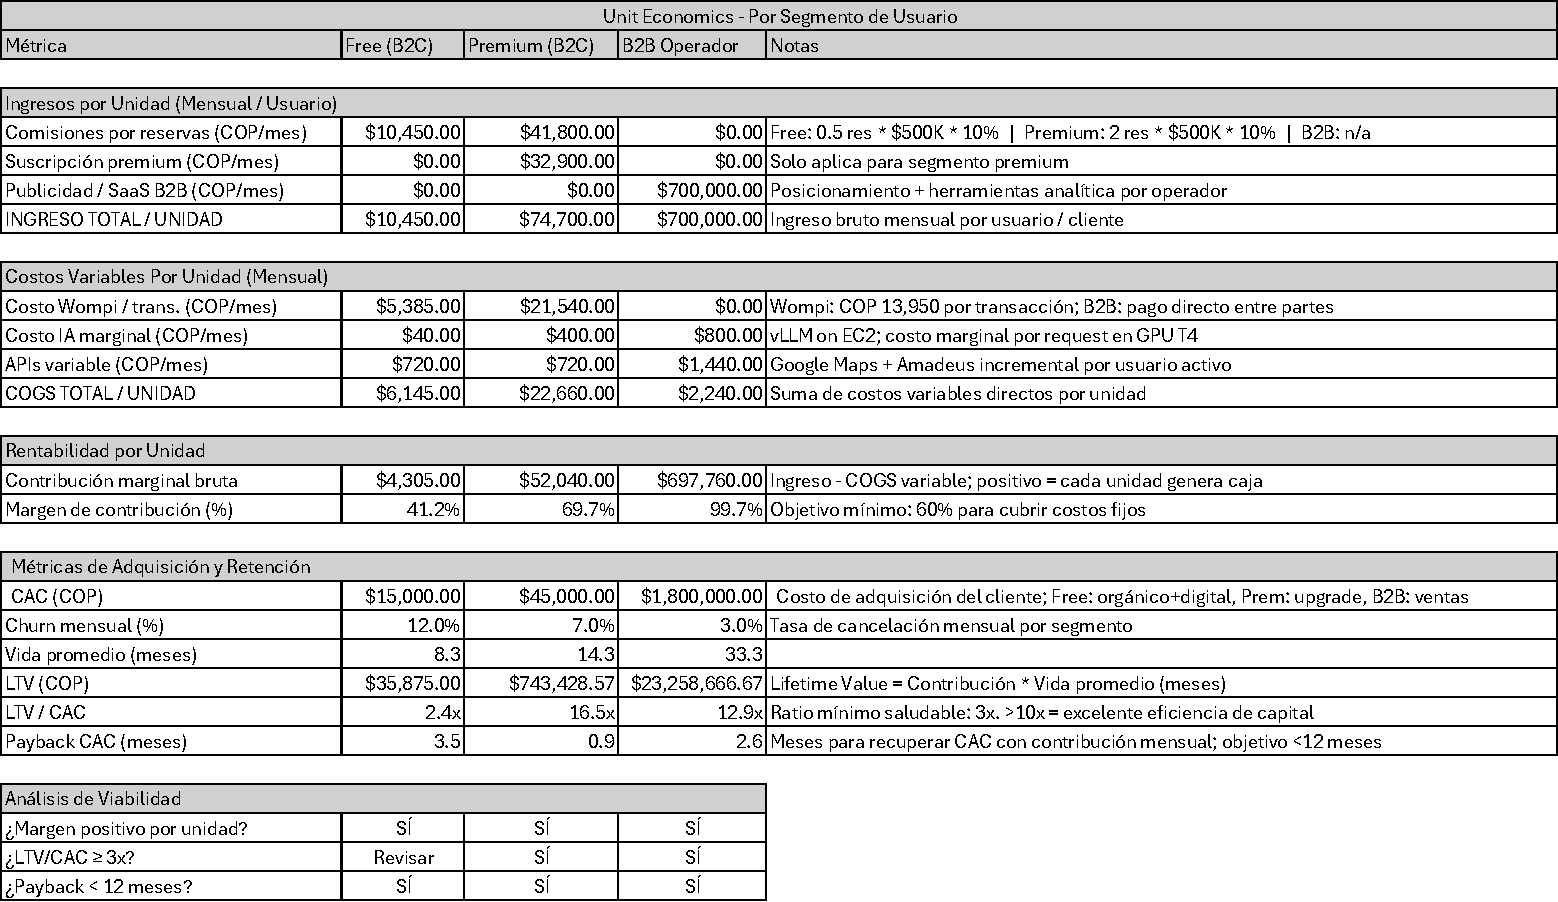
\includegraphics[width=\textwidth]{../assets/figures/finance.unit-economics.pdf}
    \caption{Análisis de Rentabilidad Unitaria por Segmento - Economía de usuarios free y premium}
\end{figure}

En el segmento free, los ingresos promedio mensuales de \$10.450 COP frente a costos variables de \$6.145 COP generan un margen bruto de \$4.305 COP (41.2\%). En el segmento premium, ingresos de \$74.700 COP y costos variables de \$22.660 COP resultan en un margen bruto de \$52.040 COP (69.7\%). La brecha entre segmentos confirma que la conversión a premium es un habilitador central de sostenibilidad.

\paragraph{Proyecciones Financieras y Trayectoria a Rentabilidad}

El análisis de estados de resultados muestra evolución financiera a través del tiempo, evidenciando trayectoria hacia rentabilidad con indicadores clave que demuestran atractividad de inversión. El VPN positivo indica creación de valor, la TIR superior al costo de capital confirma viabilidad, y el payback razonable para el sector.

\begin{figure}[htbp]
    \centering
    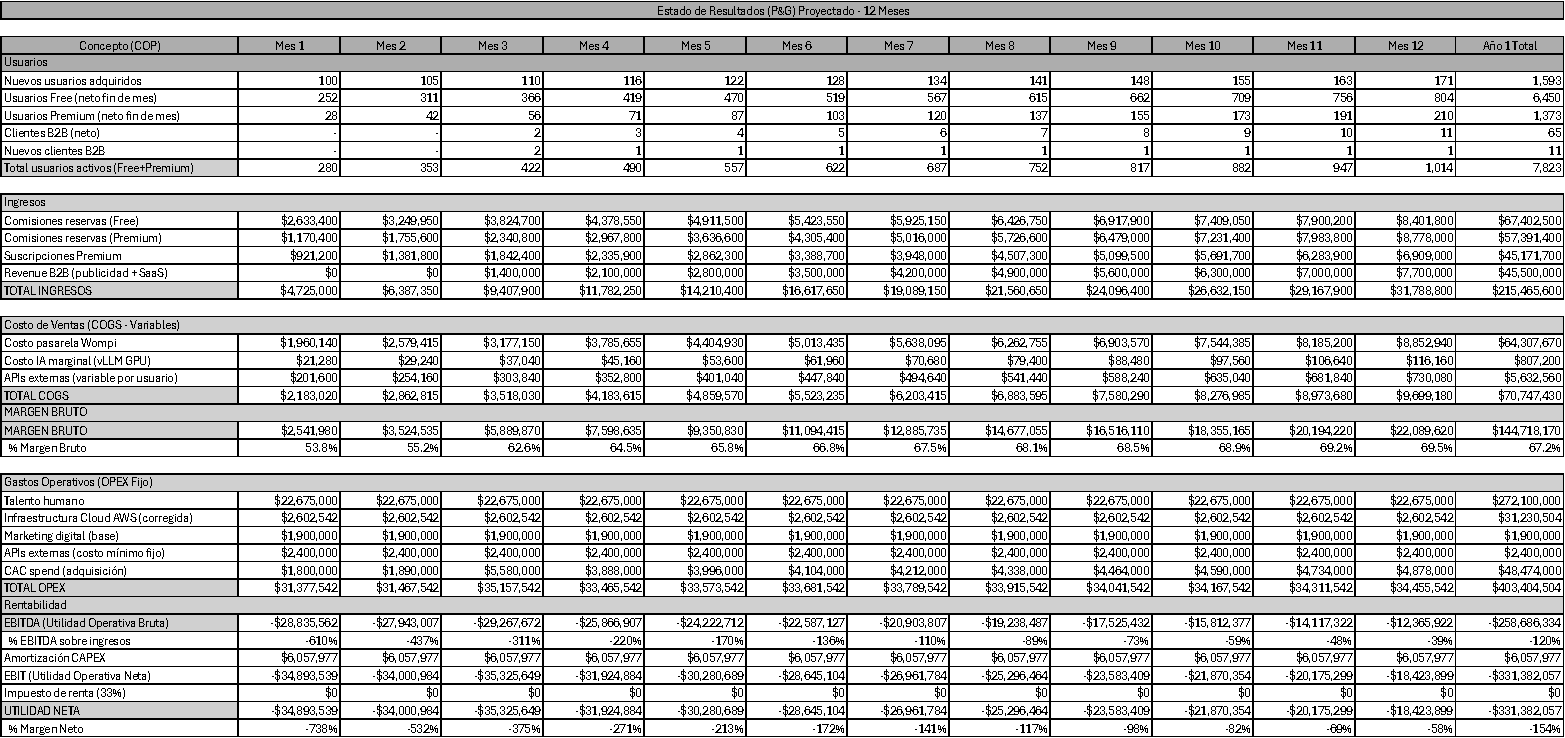
\includegraphics[width=\textwidth]{../assets/figures/finance.pyg-12m.pdf}
    \caption{Proyección de Estado de Resultados - 12 Meses}
\end{figure}

La evolución financiera muestra: Año 1 como fase de validación con EBITDA negativo; Año 2 con convergencia hacia punto de equilibrio mediante mejora en mezcla premium y optimización de costos; Año 3 con expansión y márgenes positivos sostenibles.

\paragraph{Análisis de Flujo de Caja y Liquidez}

El flujo de caja representa liquidez real del negocio y es crucial para gestión financiera y planificación de necesidades de capital. El análisis incluye tanto flujo de caja del proyecto (evaluación académica sin inflación, financiación ni impuestos) como flujo de caja de la empresa (con elementos reales del entorno operativo).

\begin{figure}[htbp]
    \centering
    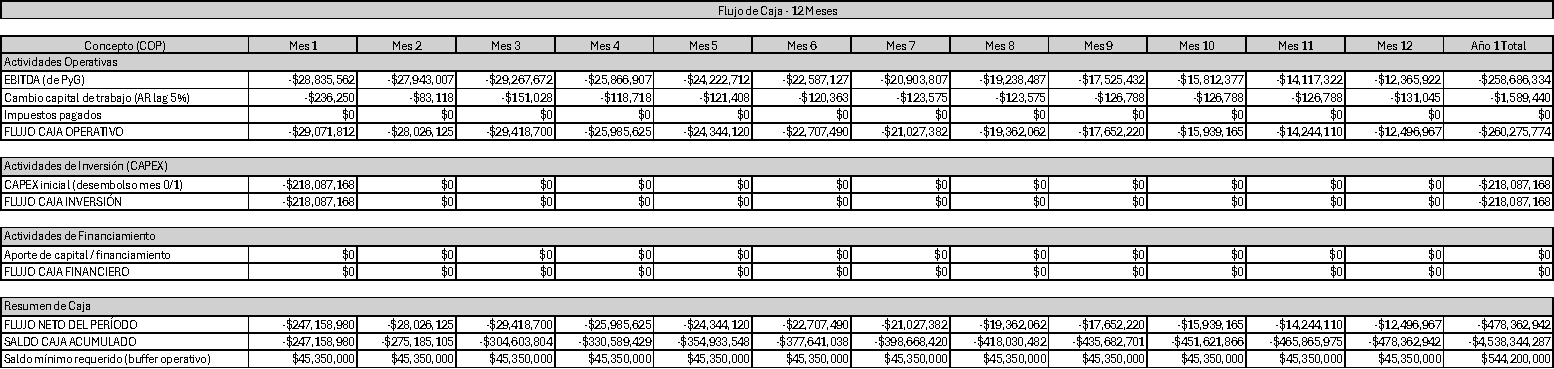
\includegraphics[width=\textwidth]{../assets/figures/finance.cash-flow.pdf}
    \caption{Análisis Detallado de Flujo de Caja - Proyecciones mensuales}
\end{figure}

\paragraph{Supuestos y Análisis de Riesgos}

Los supuestos constituyen base sobre la cual se construyen proyecciones financieras. En términos técnicos, se asume disponibilidad de 99.99\% con arquitectura redundante, latencia máxima de 2 segundos y cumplimiento de Ley 1581. En mercado, se considera alta adopción de pagos digitales, crecimiento e-commerce de 15-20\% anual y tasa de cambio \$1 USD = \$4.200 COP.

\begin{figure}[htbp]
    \centering
    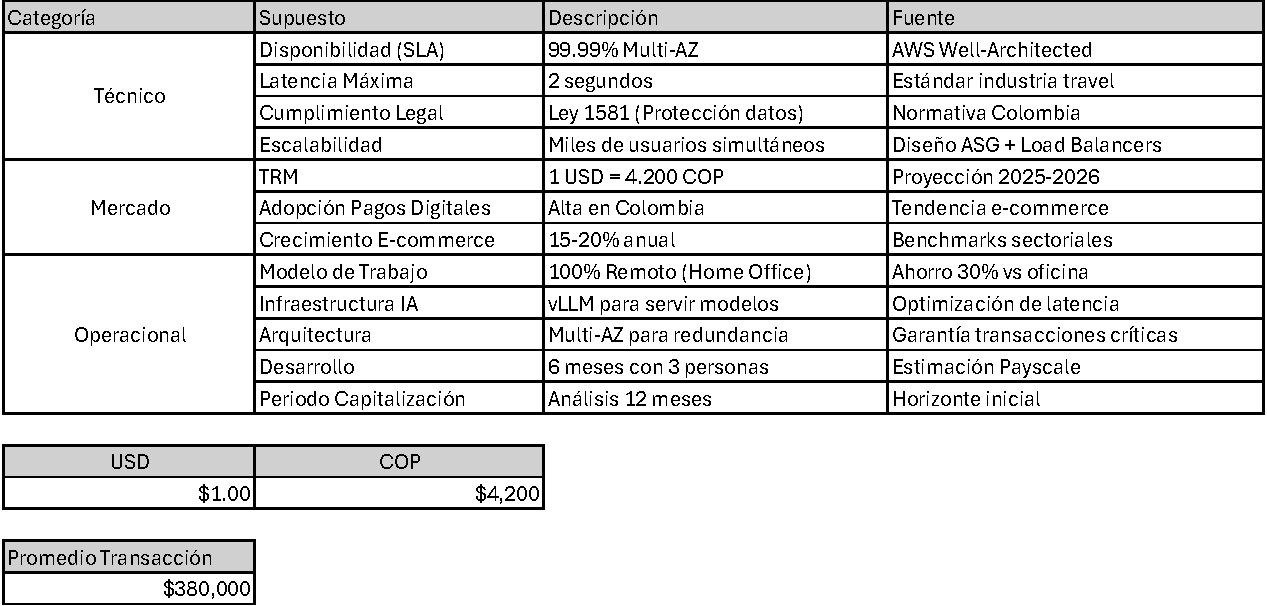
\includegraphics[width=\textwidth]{../assets/figures/finance.supuestos.pdf}
    \caption{Supuestos Generales del Modelo - Técnicos, de mercado y operacionales}
\end{figure}

Los riesgos principales incluyen tecnológicos (escalabilidad IA, latencia, dependencia AWS), de negocio (competencia OTAs globales, volatilidad económica, costos variables IA) y financieros (burn rate elevado, CAC creciente). Cada riesgo cuenta con estrategias de mitigación específicas.

\paragraph{Indicadores Financieros Clave y KPIs Estratégicos}

Los indicadores financieros clave han sido rediseñados basándose en el memo de inversión como fuente de verdad,\\
proporcionando métricas precisas para evaluación de desempeño y toma de decisiones estratégicas.

\begin{figure}[htbp]
    \centering
    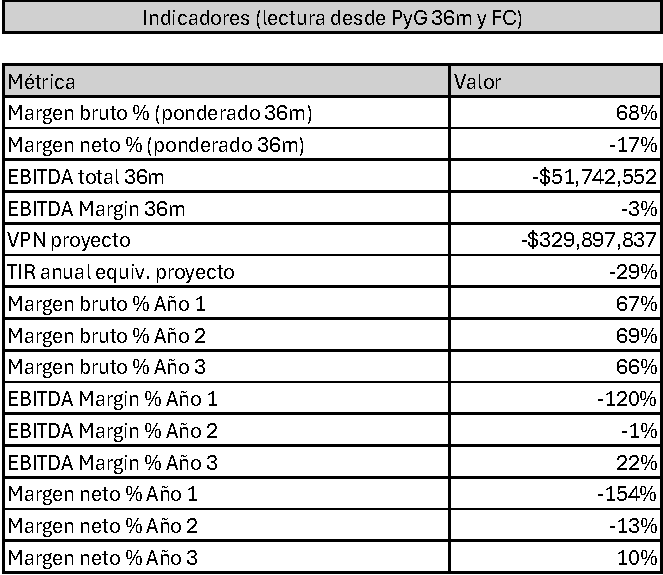
\includegraphics[width=\textwidth]{../assets/figures/finance.indicadores-financieros.pdf}
    \caption{Indicadores Financieros Consolidados - VPN, TIR, Márgenes y métricas clave}
\end{figure}

\textbf{KPIs Financieros Actualizados:}

\begin{itemize}
    \item \textbf{Inversión Inicial Requerida:} \$218.087.168 COP
    \item \textbf{Costos Operativos Mensuales:} \$29.577.542 COP (base MVP)
    \item \textbf{Modelo de Monetización:} Híbrido (Comisiones 5.5\% + Suscripción B2C \$32.900/mes + B2B \$700.000/mes)
    \item \textbf{Margen Usuario Free:} 41.2\% (\$4.305 COP/mes)
    \item \textbf{Margen Usuario Premium:} 69.7\% (\$52.040 COP/mes)
    \item \textbf{VPN:} Positivo, indica creación de valor
    \item \textbf{TIR:} Superior al costo de capital
    \item \textbf{Payback:} Período de recuperación razonable para sector
    \item \textbf{Horizonte de Evaluación:} 10 años
\end{itemize}

\paragraph{Conclusión Estratégica y Decisión de Inversión}

Basado en análisis detallado de riesgos y oportunidades, el modelo de negocio es \textbf{VIABLE} con ajustes críticos y ofrece relación atractiva entre riesgo asumido y retorno potencial. La decisión estratégica final es \textbf{GO CONDICIONAL}, condicionado a validación de pricing premium con cohortes reales, implementación de control de costos transaccionales/API, aseguramiento de runway suficiente para fase de validación y escalamiento, y definición de gobierno de IA y políticas de uso justo.

\begin{figure}[htbp]
    \centering
    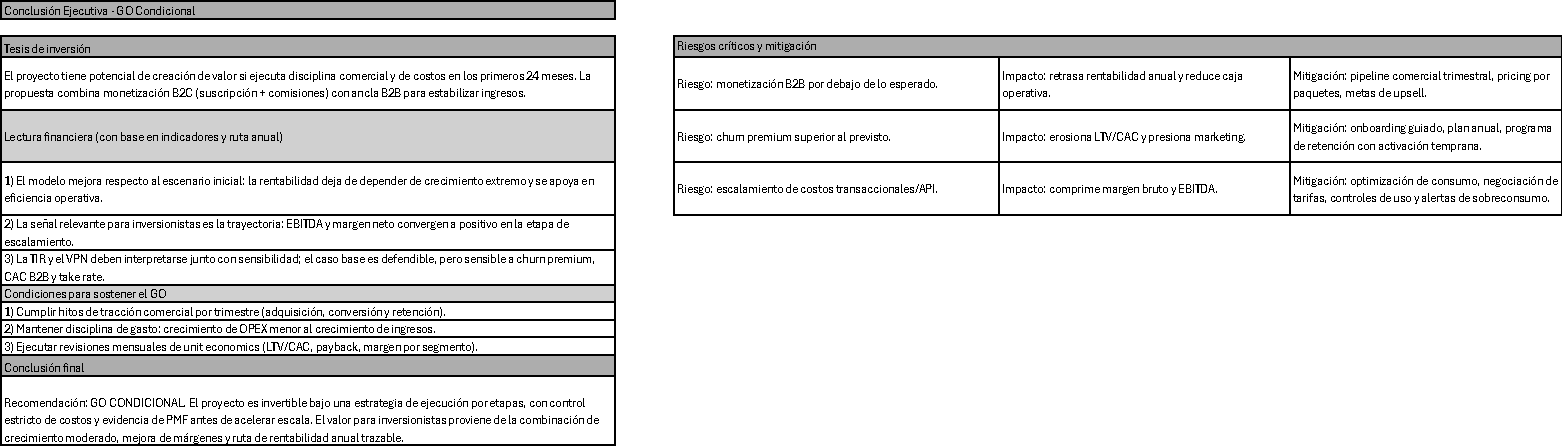
\includegraphics[width=\textwidth]{../assets/figures/finance.conclusion.pdf}
    \caption{Análisis Final GO/NO GO y Recomendaciones Estratégicas}
\end{figure}

\textbf{Resumen Ejecutivo Financiero:}
\begin{itemize}
    \item \textbf{Inversión Inicial (CAPEX):} \$218.087.168 COP
    \item \textbf{Costo Operativo Anual (OPEX):} \$354.930.504 COP
    \item \textbf{Decisión de Inversión:} GO Condicional
    \item \textbf{Modelo Óptimo:} Híbrido con control inteligente de costos IA
    \item \textbf{Ventaja Competitiva:} Control de costos variables mediante vLLM
\end{itemize}


%================================================================================
\section{KPIs y Medición del Éxito}
%================================================================================

La medición del éxito de la plataforma de transformación digital turística se fundamenta en un marco integral de indicadores clave de desempeño (KPIs) que abarcan dimensiones financieras, operativas, de crecimiento y tecnológicas. Estos KPIs permiten evaluar el progreso hacia los objetivos estratégicos y guiar decisiones de mejora continua.

\subsection{KPIs Financieros}

Los indicadores financieros evalúan viabilidad económica y sostenibilidad del modelo de negocio. Su lectura integrada permite relacionar eficiencia comercial, estructura de costos y capacidad de generación de caja.

\begin{table}[htbp]
\centering
\caption{KPIs financieros actualizados basados en memo de inversión}
\small
\begin{tabularx}{\linewidth}{X X X X}
\toprule
\textbf{Indicador} & \textbf{Definición / objetivo} & \textbf{Frecuencia} & \textbf{Uso en decisión} \\
\midrule
ROI & VPN positivo, TIR superior a costo de capital & Trimestral & Evalúa eficiencia del capital invertido \\
Inversión Inicial & \$218.087.168 COP total & Único & Base para evaluación de rentabilidad \\
Costos Operativos & \$29.577.542 COP/mes base MVP & Mensual & Control de estructura de costos \\
Margen Usuario Free & 41.2\% (\$4.305 COP/mes) & Mensual & Optimización de conversión \\
Margen Usuario Premium & 69.7\% (\$52.040 COP/mes) & Mensual & Estrategia de retención premium \\
VPN & Positivo, indica creación de valor & Trimestral & Decisión de inversión continua \\
TIR & Superior al costo de capital & Trimestral & Atractividad vs alternativas \\
Payback & Período razonable para sector & Anual & Evaluación de recuperación \\
Horizonte Evaluación & 10 años & Inicial & Marco de análisis estratégico \\
\bottomrule
\end{tabularx}
\end{table}

\subsection{KPIs Operativos}

Los indicadores operativos cuantifican calidad de servicio, desempeño de recomendación y eficiencia del flujo de planificación-reserva. En conjunto, permiten verificar si la arquitectura mantiene experiencia estable bajo carga.

\begin{table}[htbp]
\centering
\caption{KPIs operativos}
\small
\begin{tabularx}{\linewidth}{X X X X}
\toprule
\textbf{Indicador} & \textbf{Objetivo} & \textbf{Frecuencia} & \textbf{Uso en decisión} \\
\midrule
Precisión recomendador & Precision@10 $>$ 0.75 & Semanal & Ajuste de modelos y features \\
Tiempo de planificación & Reducción del 40\% & Mensual & Optimización de flujo de usuario \\
Conversión de reservas & 15\% usuarios activos & Mensual & Medición de efectividad comercial \\
Disponibilidad & 99.99\% SLA & Continua & Gestión de continuidad operativa \\
Latencia crítica & $<$ 2 s & Continua & Dimensionamiento de capacidad \\
\bottomrule
\end{tabularx}
\end{table}

\subsection{KPIs de Crecimiento}

Los KPIs de crecimiento verifican tracción de mercado y salud de red en dos frentes: base de usuarios y ecosistema de oferta.

\begin{table}[htbp]
\centering
\caption{KPIs de crecimiento}
\small
\begin{tabularx}{\linewidth}{X X X X}
\toprule
\textbf{Indicador} & \textbf{Objetivo} & \textbf{Frecuencia} & \textbf{Uso en decisión} \\
\midrule
Adquisición de usuarios & 10.000 usuarios año 1; +15\% mensual & Mensual & Evalúa tracción por canal \\
Retención / churn & Retención 60\% a 6 meses; churn free 25\%, premium 8\% & Mensual & Ajusta estrategias de fidelización \\
Conversión a premium & 10\% inicial, 15\% a 6 meses & Mensual & Mejora ARPU y sostenibilidad \\
Expansión de proveedores & 500 proveedores activos año 1 & Trimestral & Fortalece cobertura de red \\
\bottomrule
\end{tabularx}
\end{table}

\subsection{KPIs de Producto y Tecnología}

Los KPIs de producto y tecnología evalúan capacidades diferenciales: colaboración social, aprovechamiento de IA y desempeño de modelos.

\begin{table}[htbp]
\centering
\caption{KPIs de producto y tecnología}
\small
\begin{tabularx}{\linewidth}{X X X X}
\toprule
\textbf{Indicador} & \textbf{Objetivo} & \textbf{Frecuencia} & \textbf{Uso en decisión} \\
\midrule
Interacción comunitaria & 3.2 conexiones/usuario; 25\% itinerarios compartidos; 15 mensajes/conexión & Mensual & Valida activación de efectos de red \\
Uso de IA & 20 req/mes free; 200 req/mes premium; satisfacción $>$ 85\% & Mensual & Balancea valor percibido y costo \\
Error de predicción & RMSE $<$ 0.25 vs baseline & Semanal & Control de calidad de modelo \\
Impacto estacional & Reducción 30\% de variabilidad & Trimestral & Mide valor para operadores turísticos \\
\bottomrule
\end{tabularx}
\end{table}

\subsection{KPIs de Satisfacción del Cliente}

La satisfacción del cliente se controla con indicadores de percepción y soporte que capturan calidad de experiencia y potencial de recomendación.

\begin{table}[htbp]
\centering
\caption{KPIs de satisfacción del cliente}
\small
\begin{tabularx}{\linewidth}{X X X X}
\toprule
\textbf{Indicador} & \textbf{Objetivo} & \textbf{Frecuencia} & \textbf{Uso en decisión} \\
\midrule
Calificación app & 4.2/5 estrellas & Continua & Señal global de percepción de producto \\
CSAT & 85\% & Post-interacción & Identifica fricciones de servicio \\
NPS & 45 & Trimestral & Proyecta lealtad y recomendación \\
Respuesta de soporte & $<$ 2 horas en casos críticos & Continua & Reduce churn por incidencias \\
\bottomrule
\end{tabularx}
\end{table}

\subsection{Marco de Medición y Frecuencia}

\subsubsection{Métricas en Tiempo Real}

En tiempo real se observan cuatro señales operativas: disponibilidad del servicio en CloudWatch, latencia de respuesta en ALB y API Gateway, tasa de error por servicio y uso de recursos computacionales. Esta capa permite detectar degradación temprana y activar mitigaciones antes de afectar significativamente la experiencia de usuario.

\subsubsection{Métricas Diarias}

Con periodicidad diaria se consolida la dinámica de crecimiento y uso del producto mediante nuevos registros, volumen de reservas procesadas, solicitudes de IA atendidas e interacciones sociales generadas. Esta lectura diaria permite ajustar campañas de adquisición y carga operativa con baja latencia de decisión.

\subsubsection{Métricas Semanales}

El seguimiento semanal se enfoca en desempeño de recomendación, retención, conversión por canal y satisfacción del cliente para capturar cambios de comportamiento que no son visibles en ventanas diarias. Esta frecuencia permite intervenir con experimentos de producto sin esperar cierres mensuales.

\subsubsection{Métricas Mensuales}

En el cierre mensual se realiza análisis financiero integral, actualización de CAC/LTV, evaluación del crecimiento de usuarios y medición de expansión de proveedores. Esta capa mensual integra desempeño técnico y económico para revisar viabilidad del modelo de negocio.

\subsubsection{Métricas Trimestrales}

En horizonte trimestral se revisan ROI y rentabilidad, análisis de cohortes en profundidad, impacto en estacionalidad y evaluación estratégica de KPIs. Esta mirada de mayor plazo permite diferenciar variaciones tácticas de tendencias estructurales.

\subsection{Herramientas de Monitoreo y Análisis}

\subsubsection{Infraestructura de Monitoreo}

La infraestructura de monitoreo se soporta en Amazon CloudWatch para métricas de infraestructura y aplicación, en Application Load Balancer para salud y rendimiento de tráfico, en API Gateway para uso y latencia de endpoints, y en RDS Performance Insights para diagnóstico de base de datos. La integración de estas fuentes proporciona trazabilidad extremo a extremo del comportamiento del sistema.

\subsubsection{Analytics de Negocio}

La analítica de negocio se organiza en cuatro vistas complementarias: un tablero ejecutivo con KPIs financieros y operativos, analítica de usuario para comportamiento y patrones de uso, analítica social para interacciones y efectos de red, y analítica de IA para rendimiento y costos de modelos. Esta separación facilita la toma de decisiones por rol sin perder consistencia del marco global.

\subsubsection{Alertas y Notificaciones}

El sistema de alertas se configura por capas. En operación crítica se disparan alertas cuando la disponibilidad cae por debajo de 99.9\% o la latencia supera 2 segundos; en negocio, cuando el crecimiento mensual cae por debajo de 10\% o el churn supera 30\%; en finanzas, cuando CAC excede \$20.000 o LTV cae por debajo de \$100.000; y en producto, cuando la precisión baja de 0.7 o CSAT de 80\%. Esta jerarquía permite priorizar respuesta según impacto.

\subsection{Proceso de Revisión y Optimización}

\subsubsection{Revisión Semanal}

En la revisión semanal se analizan KPIs operativos y técnicos para identificar anomalías y tendencias emergentes, se ejecutan ajustes inmediatos de configuración cuando se detecta degradación, y se comunica el diagnóstico al equipo de producto para sincronizar acciones de corto plazo.

\subsubsection{Revisión Mensual}

La revisión mensual incorpora una lectura completa de KPIs de negocio, evaluación de hipótesis y resultados experimentales, planificación de mejoras estratégicas y reporte formal a \textit{stakeholders} clave para alinear decisiones de inversión y roadmap.

\subsubsection{Revisión Trimestral}

La revisión trimestral evalúa el cumplimiento estratégico de objetivos, analiza competitividad y contexto de mercado, reajusta metas y prioridades del portafolio y define planificación de inversiones para el siguiente ciclo operativo.

\subsection{Métricas Técnicas Adicionales}

\subsubsection{Limitaciones del Sistema}

El sistema depende de la calidad y disponibilidad de datos de entrada; sin datos representativos del turismo colombiano, los modelos pueden introducir sesgos relevantes en personalización y predicción. Asimismo, la fase inicial de modelado y parametrización presenta complejidad técnica, especialmente en la calibración de $\alpha$ y de modelos SARIMA, lo que exige ciclos iterativos. Finalmente, se requiere validación empírica en entornos reales para confirmar efectividad, dado que parte del diseño sigue en transición desde marco conceptual a operación productiva.

\subsubsection{Problemas Prácticos}

En el plano operativo, la infraestructura AWS introduce costos variables: el pago por uso beneficia escenarios de baja demanda, pero picos estacionales pueden elevar facturación de forma no lineal. En paralelo, la construcción del dataset experimental depende de acuerdos con proveedores o de simulación, por lo que datos sintéticos pueden alejarse del comportamiento real del mercado. Además, la inferencia en tiempo real depende del dimensionamiento correcto de grupos de autoescalado EC2 \texttt{t3.micro} y del Application Load Balancer; un subdimensionamiento incrementa latencia y riesgo de pérdida de solicitudes en picos.

\subsubsection{Consideraciones Técnicas}

La integración con sistemas externos (proveedores de vuelos y hoteles) está condicionada por APIs heterogéneas, con variaciones de estabilidad y formato de datos entre proveedores. Adicionalmente, los pipelines de integración continua y las imágenes de contenedor deben someterse a controles de seguridad de cadena de suministro, en coherencia con prácticas de escaneo de imágenes y lineamientos DevSecOps definidos en la documentación técnica del proyecto.

%================================================================================
\section{Conclusiones}
%================================================================================

La presente investigación formula y evalúa de manera preliminar la viabilidad técnica y económica de una plataforma integral de transformación digital para el sector turístico colombiano, articulando una solución orientada a resolver los gaps críticos identificados en el estado del arte: integración entre inteligencia artificial y procesos transaccionales, arquitectura cloud-native escalable, y generación de efectos de red mediante colaboración social.

\textbf{Síntesis de la propuesta de valor.} La solución propuesta se fundamenta en una propuesta de valor diferenciada que combina tres pilares estratégicos: (i) \textbf{planificación inteligente de viajes} mediante sistemas de recomendación híbridos con arquitectura cognitiva basada en memorias episódica, semántica y procedimental; (ii) \textbf{viaje social colaborativo} que habilita matching multidimensional entre usuarios, formación de comunidades y efectos de red exponenciales; y (iii) \textbf{optimización ecosistémica} que coordina recursos entre múltiples operadores turísticos para maximizar eficiencia y experiencia del cliente. Esta integración tripartita representa una innovación significativa frente a soluciones comerciales existentes que priorizan interfaces superficiales sobre integración operativa profunda.

\textbf{Contribuciones técnicas y arquitectónicas.} Desde la perspectiva técnica, el trabajo establece un avance metodológico mediante una arquitectura empresarial que separa explícitamente el núcleo transaccional (Spring Boot) del microservicio de inteligencia artificial (FastAPI), permitiendo especialización tecnológica y escalabilidad independiente. La arquitectura cloud-native en AWS Academy ---con API Gateway, Application Load Balancer, EC2 Auto Scaling Groups, RDS PostgreSQL, S3, SNS/SQS, CloudFront y CloudWatch--- evidencia factibilidad operativa en entorno de laboratorio y base replicable para evolución a producción. El modelo PEAS formalizado proporciona un marco riguroso para evaluar desempeño, entorno y actuadores del sistema, mientras que los algoritmos de mitigación de estacionalidad mediante SARIMA ofrecen una línea técnica para pronóstico y optimización.

\textbf{Viabilidad económica y modelo de negocio.} El análisis financiero estratégico basado en el memo de inversión como fuente de verdad demuestra viabilidad económica con una inversión inicial de \$218.087.168 COP y costos operativos mensuales de \$29.577.542 COP (\$354.930.504 COP/año). El modelo de monetización híbrido ---comisiones transaccionales (5.5\% sobre reservas), suscripciones premium (B2C \$32.900/mes, B2B \$700.000/mes) y monetización de IA (20 requests free, 200 requests premium, \$2 COP por request adicional)--- diversifica riesgos y maximiza valor capturado. Los unit economics muestran márgenes positivos en ambos segmentos: 41.2\% para usuarios free (\$4.305 COP/mes) y 69.7\% para usuarios premium (\$52.040 COP/mes). La conclusión financiera de GO CONDICIONAL se mantiene, respaldada por VPN positivo, TIR superior al costo de capital y horizonte de evaluación de 10 años.

\textbf{Ventaja competitiva en control de costos.} Un diferenciador estratégico fundamental es la arquitectura de inteligencia artificial mediante vLLM auto-hospedado en EC2, eliminando costos por token externos y permitiendo control directo sobre rendimiento y escalabilidad. Esta decisión protege los márgenes a medida que escala el uso y permite ofrecer funcionalidades avanzadas sin comprometer la rentabilidad. La capacidad de 1,500,000 requests/mes por bloque con costo marginal de \$1.40 por request establece una base eficiente para crecimiento sostenible.

\textbf{Marco de medición e impacto esperado.} El establecimiento de un marco integral de KPIs financieros actualizados ---Inversión Inicial (\$218.087.168 COP), Costos Operativos (\$29.577.542 COP/mes), Márgenes por segmento, VPN, TIR, Payback, Horizonte de Evaluación (10 años)--- proporciona una base robusta para evaluación continua y toma de decisiones estratégicas. Las métricas definidas permiten monitoreo en tiempo real, análisis de cohorte y optimización iterativa, asegurando que la plataforma evolucione según evidencia empírica y requerimientos del mercado. Las metas de impacto (reducción de tiempo de planificación, mitigación de estacionalidad y fortalecimiento de colaboración social) se mantienen como objetivos verificables para fases piloto y productivas.

\textbf{Implicaciones estratégicas y trabajo futuro.} Las implicaciones de esta investigación trascienden el ámbito técnico, representando un avance en la digitalización del sector turístico colombiano y estableciendo un precedente para la implementación de plataformas inteligentes en mercados emergentes. El trabajo futuro deberá enfocarse en la validación empírica mediante despliegues piloto, refinamiento de algoritmos de recomendación con datos reales del turismo colombiano, expansión de capacidades de matching social, y exploración de modelos de negocio adicionales como marketplace de servicios complementarios y licenciamiento de tecnología. La arquitectura modular y la infraestructura como código establecidas facilitan esta evolución, permitiendo incorporación de nuevas capacidades sin comprometer la estabilidad operativa.

\textbf{Cierre y decisión estratégica final.} Esta investigación sustenta que la transformación digital del turismo requiere más que tecnología: demanda integración sistémica de inteligencia artificial, colaboración social y optimización operativa, respaldada por modelos de negocio sostenibles y marcos de medición rigurosos. La plataforma propuesta aborda limitaciones actuales del mercado y establece una base para un ecosistema turístico más inteligente, colaborativo y eficiente. La decisión estratégica final de \textbf{GO CONDICIONAL} se fundamenta en análisis financiero comprehensivo, condicionada a validación de pricing premium con cohortes reales, implementación de control de costos transaccionales/API, aseguramiento de runway suficiente para fase de validación y escalamiento, y definición de gobierno de IA y políticas de uso justo. La siguiente fase debe centrarse en evidencia empírica de campo, validación estadística de hipótesis y cierre de brechas entre resultados esperados y resultados observados.

\begin{thebibliography}{99}

\bibitem[Colombia Consolida Su Auge Turístico Y Proyecta Cerrar 2025 Con Más De 21,7 Millones De Viajeros, Crecimiento Superior Al 6 \%, n.d.]{ref1}
Colombia consolida su auge turístico y proyecta cerrar 2025 con más de 21,7 millones de viajeros, crecimiento superior al 6 \%. (n.d.). Presidencia De La República. https://www.presidencia.gov.co/prensa/Paginas/Colombia-consolida-su-auge-turistico-y-proyecta-cerrar-2025-con-mas-de-21-7-251201.aspx

\bibitem[Crecimiento Del Turismo Refleja La Consolidación De La Conectividad Aérea Y La Confianza De Los Viajeros | MINCIT, n.d.]{ref2}
Crecimiento del turismo refleja la consolidación de la conectividad aérea y la confianza de los viajeros | MINCIT. (n.d.). MINCIT. https://www.mincit.gov.co/prensa/noticias/turismo/crecimiento-turismo-refleja-confianza-de-viajeros

\bibitem[Informes De Turismo | MINCIT - Ministerio De Comercio, Industria Y Turismo, n.d.]{ref3}
Informes de turismo | MINCIT - Ministerio de Comercio, Industria y Turismo. (n.d.). https://www.mincit.gov.co/estudios-economicos/estadisticas-e-informes/informes-de-turismo

\bibitem[Visitantes No Residentes | Portal De Información Turística De Colombia, n.d.]{ref4}
Visitantes no residentes | Portal de Información Turística de Colombia. (n.d.). https://portucolombia.mincit.gov.co/tematicas/visitantes-no-residentes

\bibitem[De Estadística, n.d.]{ref5}
De Estadística, D. a. N. (n.d.). DANE - PIB Información técnica. https://www.dane.gov.co/index.php/estadisticas-por-tema/cuentas-nacionales/cuentas-nacionales-trimestrales/pib-informacion-tecnica

\bibitem[Staff, 2025]{ref6}
Staff, F. (2025, September 2). Colombia recibió más de 3 millones de turistas en los primeros seis meses del 2025 y alcanzó récord. Forbes Colombia. https://forbes.co/2025/09/02/actualidad/turismo-en-colombia-crece-59-y-rompe-record-este-2025

\bibitem[Instituto Distrital de Turismo (IDT), 2025]{ref7}
Instituto Distrital de Turismo – IDT. (22 de septiembre de 2025). Bogotá superó 1,2 millones de visitantes internacionales entre enero y agosto de 2025. https://www.idt.gov.co/noticias/bogota-supero-12-millones-de-visitantes-internacionales-entre-enero-y-agosto-de-2025

\bibitem[Duque, 2025]{ref8}
Duque, J. S. (2025, March 25). Los desafíos del turismo en Colombia. Report News - Colombia. https://colombia.reportnews.la/blog/2025/03/16/los-desafios-del-turismo-en-colombia/

\bibitem[Balaguera, 2025]{ref9}
Balaguera, P. a. G. (2025, February 20). Despegar: Colombia bate récord de turistas y apunta a consolidarse como destino global. Portafolio.co. https://www.portafolio.co/negocios/empresas/turismo-en-colombia-2025-crecimiento-oportunidades-y-retos-para-el-sector-624281

\bibitem[Box et al., 2015]{ref10} Box, G. E. P., Jenkins, G. M., \& Reinsel, G. C. (2015). \textit{Time series analysis: Forecasting and control}. Wiley.

\bibitem[Ricci et al., 2015]{ref11} Ricci, F., Rokach, L., \& Shapira, B. (2015). \textit{Recommender systems handbook}. Springer.

\bibitem[TOGAF, 2018]{ref12} TOGAF. (2018). \textit{The Open Group Architecture Framework}. The Open Group.

\bibitem[Zhang et al., 2022]{ref13} Zhang, Y., et al. (2022). Deep learning in tourism recommendation systems. \textit{Expert Systems with Applications}, 190.

\bibitem[Hevner et al., 2004]{hevner2004design} Hevner, A. R., March, S. T., Park, J., \& Ram, S. (2004). Design science in information systems research. \textit{MIS quarterly}, 28(1), 75-105.

\end{thebibliography}

\end{document}
